\documentclass[a4paper, 15pt]{report}
\usepackage[utf8]{inputenc}
\usepackage[italian]{babel}
\usepackage[T1]{fontenc}
\usepackage{graphicx}
\usepackage{float}
\usepackage[centertags]{amsmath}
\usepackage{amsfonts}
\usepackage{amssymb}
\usepackage{amsthm}
\usepackage{newlfont}
\usepackage{fancyhdr}
\usepackage{tesisty}

%-----------------------------------
% CUSTOM PACKAGE && ENVIROMENT SET
%-----------------------------------

%% Color Package -------------------
\usepackage{xcolor}
\definecolor{dkgreen}{rgb}{.133,.545,.133}
\definecolor{mauve}{rgb}{0.224, 0.176, 0.255}
\definecolor{NavyBlue}{HTML}{000080}
\definecolor{Azure}{HTML}{007FFF}
\definecolor{ProcessBlue}{HTML}{0085CA}
\definecolor{cobalt}{rgb}{0.0, 0.28, 0.67}
\definecolor{columbiablue}{rgb}{0.61, 0.87, 1.0}
\definecolor{celestialblue}{rgb}{0.29, 0.59, 0.82}
\definecolor{mygreen}{RGB}{28,172,0} % color values Red, Green, Blue
\definecolor{mylilas}{RGB}{170,55,241}
\definecolor{fireenginered}{rgb}{0.81, 0.09, 0.13}
\definecolor{aquamarine}{rgb}{0.5, 1.0, 0.83}
\definecolor{babyblue}{rgb}{0.54, 0.81, 0.94}
\definecolor{darkseagreen}{rgb}{0.56, 0.74, 0.56}
\definecolor{dollarbill}{rgb}{0.52, 0.73, 0.4}
\definecolor{fawn}{rgb}{0.9, 0.67, 0.44}
\definecolor{darkturquoise}{rgb}{0.0, 0.81, 0.82}
\definecolor{cambridgeblue}{rgb}{0.64, 0.76, 0.68}
\definecolor{calpolypomonagreen}{rgb}{0.12, 0.3, 0.17}
\definecolor{cadmiumgreen}{rgb}{0.0, 0.42, 0.24}
%% My special Word Package ----------
\usepackage{specialWord}

%% Link Package	---------------------
\usepackage[hyphens]{url}
\usepackage{hyperref}
%\hypersetup{
%	colorlinks=true,
%	linkcolor=black, %black, %blue,
%	filecolor=black, %magenta,      
%	urlcolor=black,
%	citecolor=black,
%	pdftitle={Tesi Magistrale Alfano},
%	pdfpagemode=FullScreen,
%}
\hypersetup{
	colorlinks=true,
	linkcolor=Azure, %black, %blue,
	filecolor=black, %magenta,      
	urlcolor=cobalt,
	citecolor=Azure,
	pdftitle={Tesi Magistrale Alfano},
	pdfpagemode=FullScreen,
}


%% Graphics Package ---------------------------------------
\usepackage{graphicx}
\graphicspath{{Pictures/}}

%% Bibliografia Package -----------------------------------
\usepackage[
style=numeric-comp,
useprefix,
style=reading,
backend=bibtex]{biblatex}
\addbibresource{BibliografiaTesi.bib}
\usepackage{csquotes}
\usepackage{etoolbox}
\apptocmd{\sloppy}{\hbadness 10000\relax}{}{}


%% Coding Package -----------------------------------------
\usepackage{listings}

% define general style
\lstdefinestyle{defaultStyle}
{
	basicstyle=\footnotesize,
	tabsize=2,
	captionpos=b,
	frame=lines,
	breaklines=true,
	keepspaces=true
}
% define C++ style
\lstdefinestyle{cppStyle}
{
	style=defaultStyle,
	% language related
	language=C++,
	keywordstyle=\color{blue},
	commentstyle=\color{dkgreen},
	stringstyle=\color{mauve},
	showstringspaces=false,
	%otherkeywords={\#include}, % do not uncomment!
	% numbering
	numbers=left,
	numberstyle=\tiny,
	emph=[1]{class,public,private},emphstyle=[1]\color{red}, %some words to emphasise
}

\lstdefinestyle{matlabStyle}{
	language=Matlab,%
	style=defaultStyle,
	breaklines=true,%
	morekeywords={matlab2tikz},
	keywordstyle=\color{blue},%
	morekeywords=[2]{1}, keywordstyle=[2]{\color{black}},
	identifierstyle=\color{black},%
	stringstyle=\color{mylilas},
	commentstyle=\color{mygreen},%
	showstringspaces=false,%without this there will be a symbol in the places where there is a space
	numbers=left,%
	numberstyle={\tiny \color{black}},% size of the numbers
	numbersep=9pt, % this defines how far the numbers are from the text
	emph=[1]{continue,break, return},emphstyle=[1]\color{red}, %some words to emphasise
%	emph=[2]{word1,word2}, emphstyle=[2]{style},    	
	%emph=[2]{word1,word2}, emphstyle=[2]{style},    
}

% Package per Box Colorati alle Equazioni e altre utility --
\usepackage{amsmath}
\usepackage{empheq}
\usepackage{mathtools}
\usepackage{changes}
\usepackage{cancel}
\newcommand{\stkout}[1]{\ifmmode\text{\sout{\ensuremath{#1}}}\else\sout{#1}\fi}

\setdeletedmarkup{\stkout{#1}}
\setdeletedmarkup{\cancel{#1}}

\usepackage[most]{tcolorbox}
\newtcbox{\mathCalc}[1][]{
	nobeforeafter, math upper, tcbox raise base,
	enhanced, colframe=blue!30!black,
	colback=cyan!20, boxrule=1pt,#1
}

\newtcbox{\mathResult}[1][]{
	nobeforeafter, math upper, tcbox raise base,
	enhanced, colframe=blue!30!black,
	colback=columbiablue, boxrule=1pt,#1
}

\newtcbox{\mathStep}[1][]{
	nobeforeafter, math upper, tcbox raise base,
	enhanced, colframe=blue!30!black,
	colback=white, boxrule=1pt,#1
}

% Package per Liste -----------------------------------------
\usepackage{enumitem}

% Package per aggiungere il tab -----------------------------
\usepackage{tabto}   


% Package per aggiungere box colorati -----------------------
\usepackage{mdframed}

% Package per usare le colonne multiple ---------------------
\usepackage{multicol}
\usepackage{vwcol}  

% Package per fare tabelle più complesse --------------------
\usepackage[thinlines]{easytable}

% Package per Numeri in formato esponenziale ----------------
\usepackage{siunitx}


%-------------------------------
% DEFINIZIONE DEGLI ENVIRONMENT
%-------------------------------
\usepackage{setspace}

\newtheorem{obs}{Osservazione}[section]
\newenvironment{oss}
{\begin{mdframed}[backgroundcolor=fawn!40]\begin{obs}\begin{normalfont}}
			{\phantom{. .}\hfill$\square \!\!\!\!\checkmark$ \end{normalfont}\end{obs}\end{mdframed}}

\newtheorem{pro}{Problema}[chapter]
\newenvironment{prob}
{\begin{pro}\begin{normalfont}}
		{\hfill $\spadesuit$ \end{normalfont}\end{pro}}

\newtheorem{teor}{Teorema}[section]
\newenvironment{teorema}[1][thName]
{\begin{mdframed}[backgroundcolor=gray!10]\begin{teor}[#1]\hfill\textit\break }
		{\hfill $\blacksquare$ \end{teor}\end{mdframed}}

\newtheorem{defn}{Definizione}[section]
\newenvironment{de}[1][defName]
{\begin{mdframed}[backgroundcolor=blue!10] \begin{defn}[#1]\hfill\begin{spacing}{1.0}\begin{normalfont}}
				{\hfill $\clubsuit$ \end{normalfont}\end{spacing}\end{defn}\end{mdframed}}

\newenvironment{leg}
{\begin{mdframed}[backgroundcolor=cyan!10]\begin{itemize} [topsep=0pt,itemsep=0mm, leftmargin=2mm]}
		{\end{itemize}\end{mdframed}}


\renewcommand\lstlistlistingname{Elenco dei codici}


%-----------------------------
% CONFIGURAZIONE DELLA PAGINA
%-----------------------------

\hfuzz2pt % Don't bother to report over-full boxes if over-edge is < 2pt

\fancypagestyle{plain}{
\fancyhead{}\renewcommand{\headrulewidth}{0pt} } \pagestyle{fancy}
\renewcommand{\chaptermark}[1]{\markboth{\small CAP. \thechapter \textit{ #1}} {} }
\renewcommand{\sectionmark}[1]{\markright{\small  \thesection \textit{ #1}} {} }
\voffset=-20pt    % distanza tra il limite superiore del foglio e l'intestazione
\headsep=40pt     % distanza  l'intestazione ed il testo del corpo
\hoffset=0 pt     % misura equivalente al margine sinistro
\textheight=620pt % altezza del corpo del testo
\textwidth=435pt  % larghezza del corpo del testo
\footskip=40pt    % distanza tra il testo del corpo ed il pie' di pagina
\fancyhead{}      % cancella qualsiasi impostazione per l'intestazione
\fancyfoot{}      % cancella qualsiasi impostazione per il pie' di pagina
\headwidth=435pt  % larghezza del'intestazione e del pie' di pagina
\fancyhead[R]{\rightmark} \fancyfoot[L]{\leftmark}
\fancyfoot[R]{\thepage}
\renewcommand{\headrulewidth}{0.3pt}   % spessore della linea dell'intestazione
\renewcommand{\footrulewidth}{0.3pt}   % spessore della linea del pi�di pagina

\numberwithin{equation}{section}
\renewcommand{\theequation}{\thesection.\arabic{equation}}




%--------------------------
% MODIFICARE DA QUI IN POI
%--------------------------

\begin{document}

\dedicate{{
		Dedico questo traguardo ai miei cari nonni, e alla mia professoressa Beniamina\\
		che sempre hanno saputo esserci per me e a voi affido i traguardi di domani.
		}}
\corso{DELL'AUTOMAZIONE}
\titoloTesi{
	Sviluppo di un mokup per la prototipazione \\ di architetture di controllo per Tokamak.
} \anno{2020/2021}
\relatore{Daniele Carnevale}
\autore{Emanuele Alfano}
\correlatore{Marco Passeri}

\baselineskip=25pt

\intestazione

%------------------------------------------------
% INTRODUZIONE E RINGRAZIAMENTI (NON MODIFICARE)
%------------------------------------------------

\fancypagestyle{plain}{
	\fancyhead{}\renewcommand{\headrulewidth}{0pt} } \pagestyle{fancy}
\renewcommand{\chaptermark}[1]{\markboth{\small Cap. \thechapter \textit{ #1}} {} }
\renewcommand{\sectionmark}[1]{\markright{\small  \S \thesection \textit{ #1}} {} }
\voffset=-20pt                         % distanza tra il limite superiore del foglio e l'intestazione
\headsep=40pt                          % distanza  l'intestazione ed il testo del corpo
\hoffset=0pt                           % misura equivalente al margine sinistro
\textheight=620pt                      % altezza del corpo del testo
\textwidth=435pt                       % larghezza del corpo del testo
\footskip=40pt                         % distanza tra il testo del corpo ed il pie' di pagina
\fancyhead{}                           % cancella qualsiasi impostazione per l'intestazione
\fancyfoot{}                           % cancella qualsiasi impostazione per il pie' di pagina
\headwidth=435pt                       % larghezza del'intestazione e del pie' di pagina
\fancyhead[R]{\rightmark} \fancyfoot[L]{\leftmark}
\fancyfoot[R]{\thepage}
\renewcommand{\headrulewidth}{0.3pt}   % spessore della linea dell'intestazione
\renewcommand{\footrulewidth}{0.3pt}   % spessore della linea del pi�di pagina

\pagenumbering{Roman}

%---------------------
%     Inizio Tesi
%---------------------

% Indice SENZA link colorati
{
	\hypersetup{hidelinks}% Rimuove la colorazione per i Link
	\tableofcontents
}
\newpage

\pagenumbering{arabic}



\fancyhead[R]{Introduzione} \fancyfoot[L]{Introduzione}
\fancyfoot[R]{\thepage}

\chapter*{Ringraziamenti}
\addcontentsline{toc}{chapter}{Ringraziamenti}
\vspace{-8mm}
Questa tesi è stata resa possibile dal contributo nella mia vita di tante persone, che giorno per giorno mi hanno sempre dato il loro sostegno, a voi dedico questa mia Tesi.\\
Un ringraziamento speciale alla mia famiglia, in particolare a mia \textbf{Madre} e mio \textbf{Padre}: è grazie al vostro sostegno e incoraggiamento se oggi sono riuscito a raggiungere questo traguardo.\\
La forza di arrivare qui, oggi, però non è dovuta solo a loro, devo per forza ringraziare dell'affetto e il sostegno speciale da parte dei miei cari amici, che ogni giorno hanno condiviso con me gioie, sacrifici e successi, senza voltarmi mai le spalle, mi hanno dato la forza di arrivare a questo prezioso traguardo. \textbf{Filippo}, \textbf{Gabriele}, \textbf{Marta}, grazie di TUTTO.\\
Un pensiero in particolare vola verso la mia dolce \textbf{\textit{Nicoleta}}, è sicuramente grazie all'affetto e le attenzioni che mi hai donato che sono riuscito a tenere dritto il timone ed arrivare qui oggi.
Per terminare voglio ringraziare tutti i professori che negli ultimi 18 anni hanno guidato il mio cammino, loro che hanno sempre creduto in me e nelle mie capacità meritano tutta la mia gratitudine.\\
Un ringraziamento speciale va però alla mia professoressa e mentore \textbf{Beniamina Rauch} che fu la prima a vedere il mio potenziale e coltivarlo, so che ancora vegli su di me, non troverò mai le parole per ringraziarti abbastanza.\\
Oltre a lei ringrazio il mio relatore \textbf{Daniele Carnevale} che in questi anni universitari, da quando mi ha conosciuto ad oggi, ha sempre creduto in me e mi ha permesso di fare esperienze che mai avevo immaginato.\\ \\
Un sentito grazie a tutti voi e buona lettura.


\chapter*{Introduzione}
\addcontentsline{toc}{chapter}{Introduzione}
La tesi si colloca nell'ambito delle tecniche di controllo per impianti Tokamak, come FTU (Frascati Tokamak Upgrade), Proto-Sphera ed ITER (International Thermonuclear Experimental Reactor).\\
Essa è stata realizzata in collaborazione con il centro ricerche \textbf{ENEA} (Ente Nazionale per l’Energia e l’Ambiente) di Frascati e coordinato dal gruppo \textbf{CODAS} (COntrol and Data Acquisition System).\\
L'obiettivo finale del CODAS è di replicare in miniatura un intero impianto Tokamak, con particolare attenzione al prototipo dell'architettura software per il monitoraggio e controllo dell'esperimento.\\
In questa tesi viene discussa la creazione e lo sviluppo del prototipo della scheda embedded da usare per pilotare la corrente delle bobine magnetiche, generando così il confinamento magnetico del Plasma necessario alla reazione di fusione nucleare, presente all'interno del Tokamak.


\section*{Cos'è la Fusione Termonucleare?}
\addcontentsline{toc}{section}{Cos'è la Fusione Termonucleare?}
In fisica, per \textbf{Fusione Termonucleare}, si intende il processo mediante il quale i nuclei di due o più atomi vengono compressi tanto da far prevalere l’interazione forte sulla repulsione coulombiana, causando l'unione tra gli atomi e andando a formare così un nucleo la cui massa totale risulta minore della massa dei reagenti originali. La perdita di massa ha come conseguenza la liberazione di un’elevata quantità di energia, la quale conferisce al processo caratteristiche fortemente esotermiche.\\
La massa mancante viene trasformata in energia in accordo con l’equazione di Einstein:
\begin{center}
	$E = (m_r - m)c^2$
\end{center}
Dove $ m_r $ è la massa dei reagenti e $ m $ è la massa risultante.\\
Il processo di \textbf{Fusione Nucleare} avviene naturalmente all'interno delle stelle e trasforma l'\textit{idrogeno} (di cui sono composte) in \textit{elio}.\\
L'energia nucleare prodotta a seguito di questa reazione è elevatissima e per tale motivo risulta di forte interesse per la civiltà umana sviluppare tecniche sofisticate che ne permettano la raccolta in maniera controllata.\\
Tra i vantaggi di questa tecnologia troviamo sia motivi economici che ambientali e i principali possono essere sintetizzati in:
\begin{description}
	\item [Combustibile semi-inesauribile]:\\
	      Il combustibile (idrogeno e/o deuterio) è praticamente inesauribile ed è a disposizione di tutte le nazioni che abbiano uno sbocco sul mare. Il deuterio può essere estratto dall'acqua, anche se con costi energetici non indifferenti;\\
	      per fare un esempio, un ditale pieno di deuterio equivale a 20 tonnellate di carbone in termini di energia.\\
	      Un lago di medie dimensioni contiene deuterio sufficiente a rifornire una nazione di energia per secoli utilizzando la fusione nucleare (ovviamente supponendo di sfruttarlo tutto).
	\item [Rischi di Contaminazione grave sono \underline{nulli}]:\\
	      Nessuna possibilità di incidenti come quelli di Černobyl' o di Three Mile Island in quanto il reattore non contiene sostanze radioattive come l'uranio o le scorie di fissione.\\
	      In oltre, possibili incidenti, come fughe di trizio o perdite di liquido refrigerante, avrebbero un impatto ambientale e radiativo molto più contenuto e temporaneo.
	\item [Assenza di inquinanti ambientali]:\\
	      Il processo di fusione, durante il quale gli atomi di idrogeno vengono fusi per creare elio, non rilascia nessun elemento inquinante da combustione (ad esempio anidride carbonica) e per tanto nessun residuo può essere immesso nell'atmosfera impedendo il riscaldamento del pianeta tramite l'effetto serra.
	\item [Nessuno prodotto derivato è adatto a fini Bellici]:\\
	      La mancanza di materiale radioattivo residuo, impedisce l'utilizzo dei reattori per la produzione di materiale per scopi bellici o terroristici, come proiettili radioattivi o materiale fissile per bombe nucleari.
	\item [Livelli lievi di radiottività residua]:\\
	      Il processo di fusione può rendere radioattivi solo i materiali che compongono il Tokamak e i gas usati per il Plasma, ma entrambi gli elementi possiedono un tempo di decadimento alquanto breve, il ché implica che i rifiuti radioattivi hanno una scarsa durata nel tempo, in oltre le radiazioni prodotte non sono a energie elevatissime, semplificandone il contenimento attraverso contenitori schermati più economici e sicuri.
\end{description}
\noindent
Questi e molti altri motivi rendono lo sviluppo di metodi per catturare l'energia da \textbf{Fusione Nucleare} con attraverso processi controllati di grande interesse per tutta la civiltà umana, essa potrebbe infatti essere la chiave per preservare l'ambiente del nostro pianeta e fornire al temo stesso l'energia di cui l'umanità necessita.\\
In questa tesi faremo riferimento ad una classe di impianti sperimentali per la \textbf{Fusione Nucleare Controllata}, detti "\textbf{Impianti Tokamak}". \'E doveroso specificare che essi sono solo uno dei tanti design su cui attualmente si fa ricerca e sviluppo nel mondo, ma tra le varie proposte essi sembrano essere i più promettenti per aprire le porte a questa rivoluzione, poiché il principio di base è la replica delle condizioni che generano la fusione all'interno in una stella.\\
Tolte le difficoltà tecniche per le quali infatti è ancora una tecnologia in sviluppo, abbiamo la sicurezza sperimentale della fattibilità del processo, la nostra stessa civiltà non esisterebbe se il Sole non producesse questa forma di energia al suo interno.
\newpage

\section*{Struttura di un Tokamak}
\addcontentsline{toc}{section}{Struttura di un Tokamak}
Un \textbf{Tokamak}\footnote{Tokamak è l'acronimo russo per "camera toroidale magnetica"} è una macchina di forma toroidale (a ciambella) in cui un gas (solitamente idrogeno) viene portato nello stato di Plasma e mantenuto coeso e lontano dalle pareti interne grazie ad un campo magnetico creato da elettromagneti esterni alla camera.
\begin{figure}[H]
	\centering
	\caption[Sezione di un Tokamak]{Sezione di un Tokamak}
	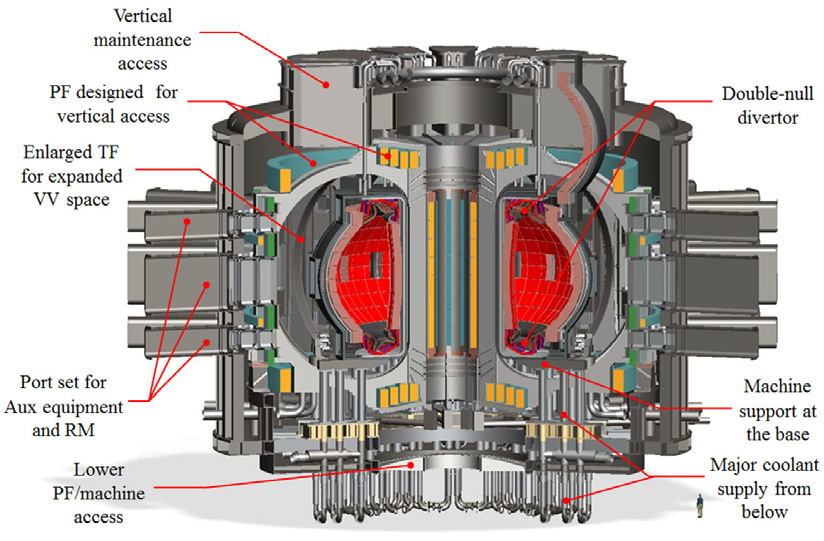
\includegraphics[width=0.65\textwidth]{Introduzione/K-DEMO_device_core_design_features.jpg}
\end{figure}

\noindent
La forma del Tokamak a \textit{toro} è studiata per permettere alle particelle del Plasma di muoversi all'interno del campo magnetico, creato all'esterno delle pareti (\textit{Esterno del Vessel}) in un moto circolare.\\
Questo movimento avviene poiché le particelle del Plasma sono per definizione cariche, e in quanto tali, se immerse in un campo magnetico esse tendono a muoversi seguendo una traiettoria elicoidale (detta anche \textit{moto di ciclotrone}) attorno alle linee del campo magnetico, che in questo caso sono chiuse e contenute all'interno della sezione del Tokamak (\textit{Interno del Vessel}).\\
L'uso di una confinazione magnetica di questo Plasma è dovuta all'impossibilità, per qualunque materiale, di resistere alle enormi temperature raggiunte dal Plasma durante la fusione in caso di un contatto diretto.\\

\noindent
La forma scelta per i Tokamak a Toro ha motivazioni fisiche, che discendono principalmente dall'equazione di Larmor. L'equazione descrive la distanza massima oltre il quale una particella carica non può allontanarsi da una linea di campo magnetico, definendo un limite superiore per lo spazio di contenimento delle particelle; questa distanza è detto appunto \textit{raggio di Larmor}:\\
\begin{vwcol}[widths={0.3,0.7}, sep=8mm, rule=1px]
	\begin{empheq}[box=\mathCalc]{equation*} \label{eq:Larmor}
		{\displaystyle \,\rho ={\frac {mv_{\perp }}{Ze\,B}}}
	\end{empheq}
	\newpage % con wcol, le colonne sono "pagine"
	\begin{spacing}{1.25}
		{\footnotesize
			$ {\displaystyle v_{\perp }} $ è la velocità della particella perpendicolare al campo magnetico.\\
			$ {\displaystyle m} $ è la sua massa.\\
			$ {\displaystyle B} $ è l'intensità del campo magnetico.\\
			$ {\displaystyle Ze} $ è la carica del portatore.
		}
	\end{spacing}
\end{vwcol}
\noindent
L'equazione vale anche in presenza di un campo magnetico curvo, se questa curva è chiusa si ottiene che la particella è confinata in uno spazio di volume finito ma rimane comunque libera ruotare all'infinito, accumulando così energia.\\
\'E stata scelta la geometria del \textbf{Toro} per rendere questa linea di campo una circonferenza esatta, la quale semplifica enormemente delle complesse equazioni fluido-dinamiche applicate al Plasma.\vspace{-5mm}
\begin{figure}[H]
	\centering
	\caption[Geometria di un Toro]{Geometria di un Toro}
	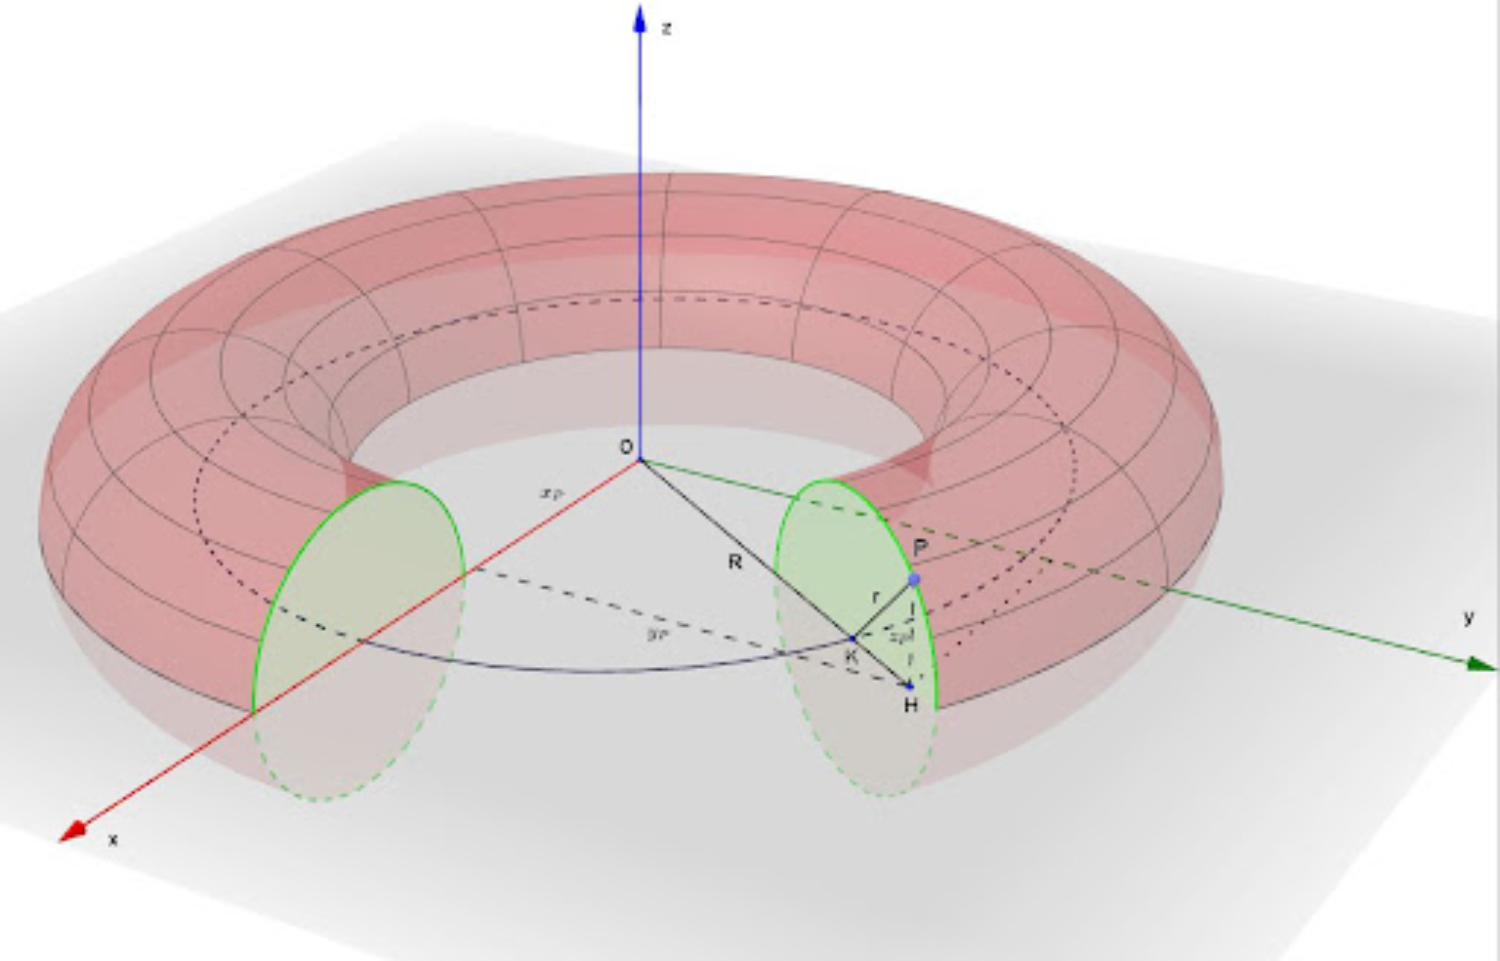
\includegraphics[width=0.65\textwidth]{Introduzione/toro-big.png}
\end{figure}\vspace{-8mm}
\noindent
In sintesi un Tokamak è un impianto progettato per creare questo confinamento magnetico in maniera efficace e sicura, e ha la forma più consona per realizzare questo processo.\\
Oltre al mero contenimento però, il secondo obiettivo è quello di compattare il Plasma su se stesso (aumentando la forza del campo magnetico $ B $), così da avvicinare di più gli atomi tra loro (l'aumento di $ B $ causa una riduzione di $ \rho $).\\
Questo aumento di pressione, unito alle alte energie immesse nel Tokamak (la cui temperatura è \textbf{di decine di volte} superiore a quella della superficie del sole) aumentano le probabilità di scontro tra gli atomi, e quindi inizio di un processo di fusione tra essi. 

\section*{Obiettivi della Tesi}
\addcontentsline{toc}{section}{Obiettivi della Tesi}
Il progetto complessivo portato avanti dall'ENEA prevede la realizzazione di prototipi a più livelli di un sistema Tokamak.\vspace{-4mm}
\begin{figure}[H]
	\centering
	\caption[Architettura Complessiva Progetto ENEA]{Architettura Complessiva Progetto ENEA}
	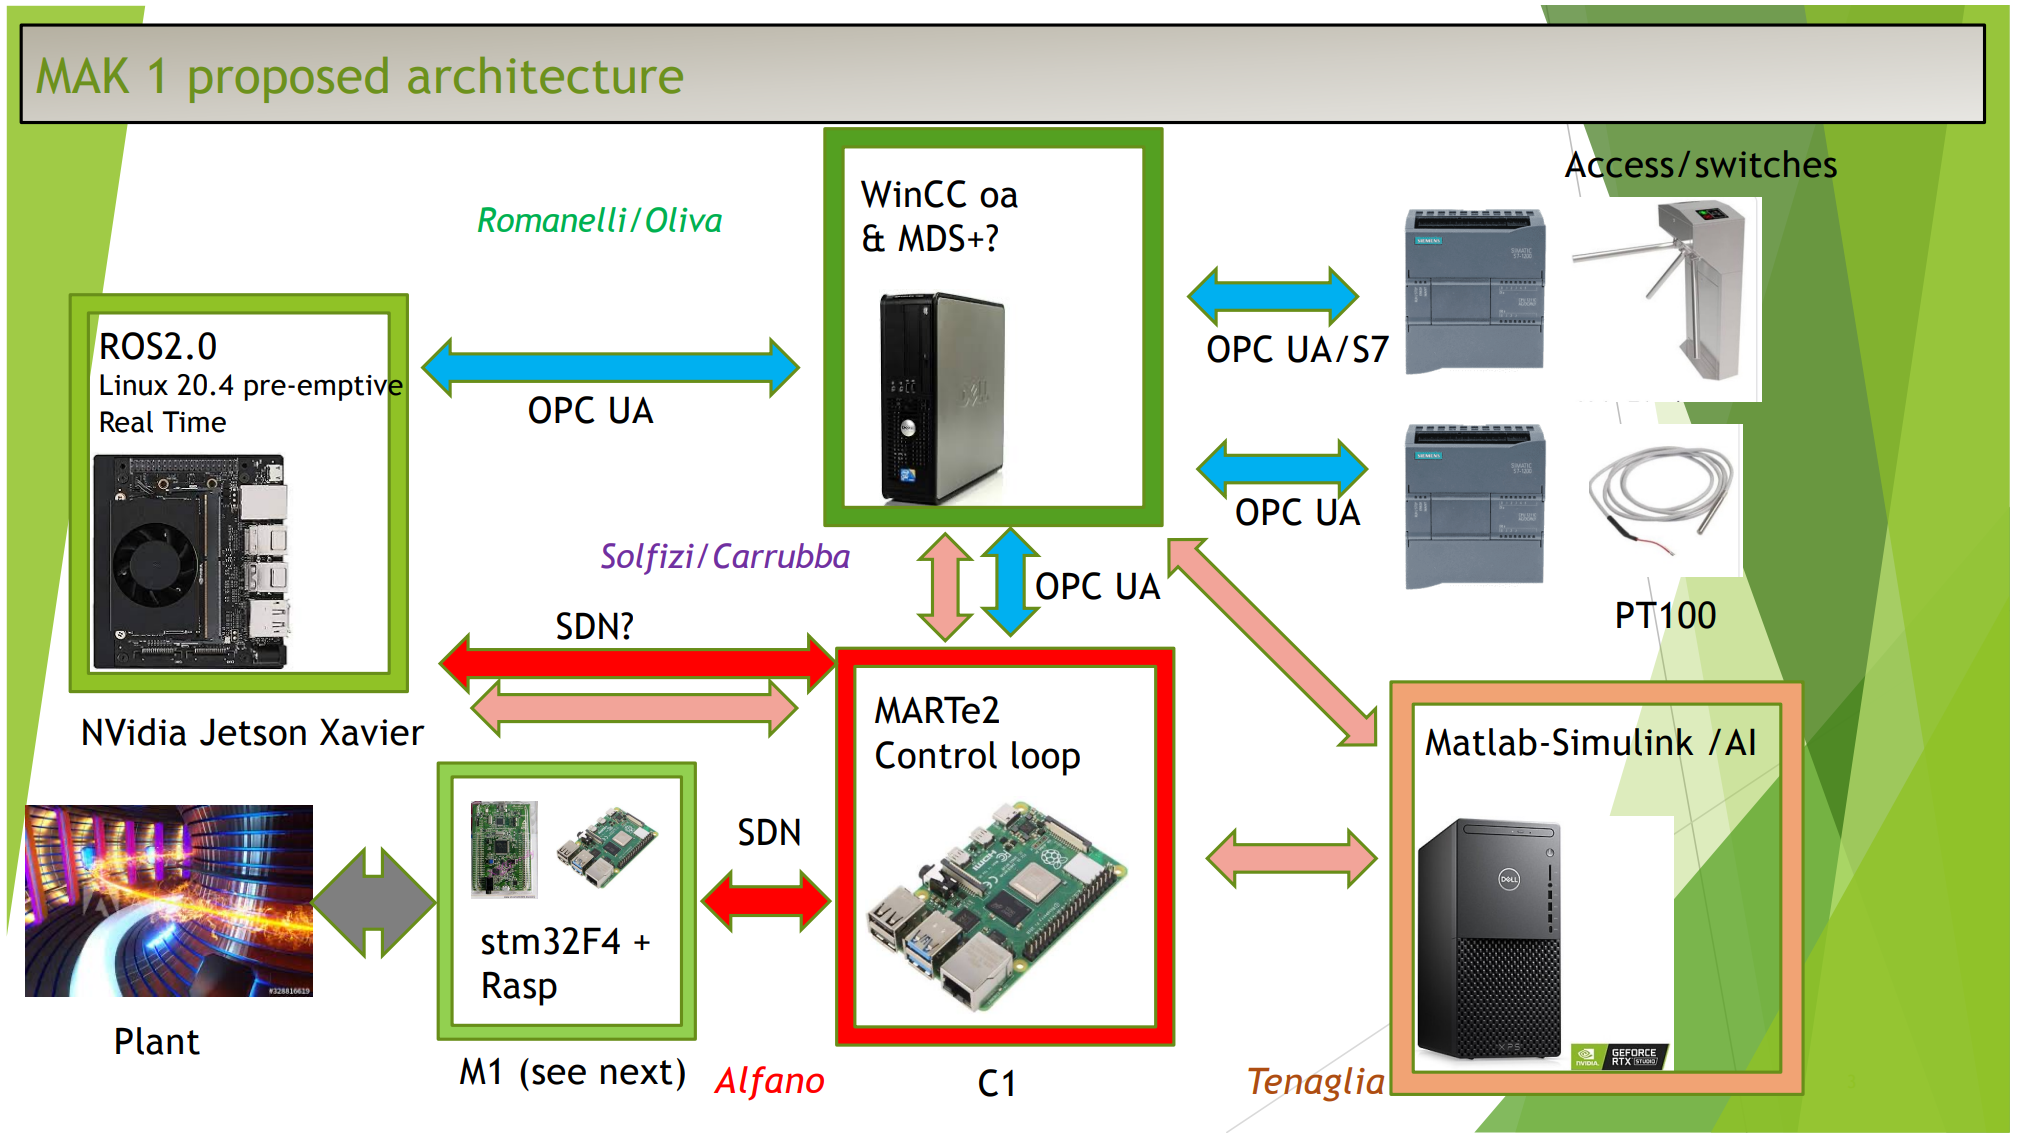
\includegraphics[width=\textwidth]{Introduzione/ArchitetturaComplessiva.png}
\end{figure}\vspace{-8mm}
\noindent
La mia parte di progetto ({\color{red}Alfano}) consiste nello sviluppare e realizzare una una scheda embedded.\\
Essa dovrà pilotare la corrente nelle bobine dell'impianto Tokamak ed essere in grado di ricevere e inseguire i riferimenti per la corrente di Plasma attraverso la rete di interconnessione tra i dispositivi, basata sul Framework di \MARTe. (argomento trattato con dettaglio nella tesi)\\
Il controllo realizzato punta a inseguire il riferimento richiesto con un errore nullo.\\
In fine il dispositivo deve essere in grado di comunicare in real-time l'attuale stato del sistema al resto della rete, per permettere una diagnostica in tempo reale dell'andamento dell'impianto.\\

\fancyhf{} %elimina header/footer vecchi


\fancyhead[R]{\rightmark} \fancyhead[L]{\leftmark}
\fancyfoot[R]{\thepage}

%---------------------
% INCLUSIONE CAPITOLI
%---------------------

\chapter{Elementi Costitutivi}\label{cap:Hardware}

\begin{minipage}{12cm}\textit{
		In questo capitolo si vogliono descrivere e caratterizzare i 3 elementi salienti dell'esperimento:
		\begin{enumerate}
			\item \nameref{TrasformatoreModelloTokamak}
			\item \nameref{CurrentSense}
			\item \nameref{CurrentDriver}
		\end{enumerate}
	}
	Essi verranno analizzati al fine di mettere in luce i loro punti di forza, ovvero i motivi che hanno portato alla loro scelta, e si evidenzieranno eventuali problemi che affliggono in componenti, problemi di cui si è tenuto conto nello sviluppo del progetto per poterli annullare e/o compensare. 
\end{minipage}

\newpage

\section{Trasformatore, un Modello di Tokamak}\label{TrasformatoreModelloTokamak}

Come visto nell'introduzione, la tesi ha come obiettivo la prototipazione del sistema di controllo per le bobine magnetiche presenti in impianti tokamak.
\begin{figure}[H]
	\centering
	\caption[Schema interno di un Tokamak]{Interno Tokamak}
	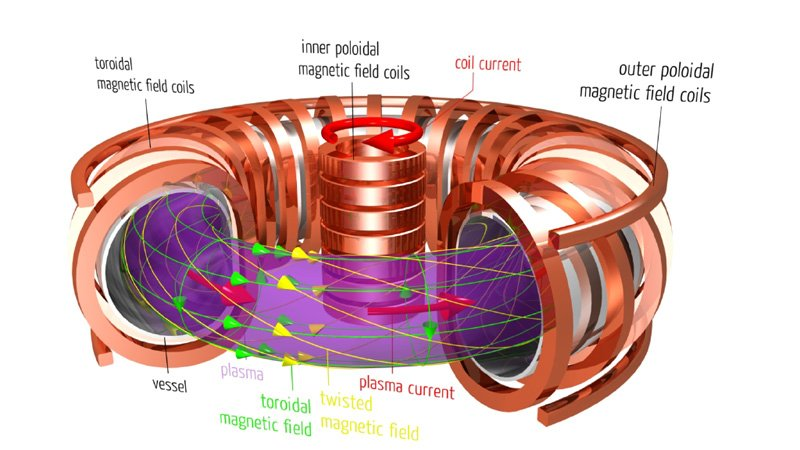
\includegraphics[width=1\textwidth]{Trasformatore/tokamak_scheme.jpg}
\end{figure}
\noindent
Le bobine (poloidali e toroidali) servono a controllare il Plasma presente nel \textit{Vessel} dell'impianto e confinare il Plasma all'interno di un flusso compresso dentro la camera, le alte temperature e la forte compressione a cui è sottoposto il Plasma, permette di realizzare eventi di \textbf{Fusione Nucleare Controllata} tra gli atomi di idrogeno che compongono il Plasma usato dentro il Tokamak.\\
Essendo però impossibile usare in un ambiente controllato un vero Tokamak, specie in un laboratorio universitario, si è usato un sistema fisico equivalente per ricreare l'interazione tra le \textbf{Bobine e il Plasma}.\\
Il modello equivalente in questione è quello di \textbf{Trasformatore Elettrico} nella relazione \textit{Primario-Secondario} (con ovviamente alcune approssimazioni e la semplificazione di varie \nonLinearita sui suoi parametri, a delle costanti).\\
Grazie a questa similitudine è stato possibile replicare in sicurezza la fisica presente all'interno di un Tokamak, nell'ambiente controllato del laboratorio usando una batteria in grado di erogare molti Ampere come fonte di alimentazione dell'esperimento.\\

\subsection{Richiami di elettronica}
Prima di modellare ed analizzare l'esperimento della tesi, è necessario richiamare qualche proprietà/concetto di elettronica per poter comprendere i passaggi matematici e fisici:
\vspace{-5mm}
\NumTabs{7}
\begin{itemize}[itemsep=-4mm]
	\item \nameref{th:KirchhoffNodi}
	\item \nameref{th:KirchhoffMaglie}
	\item \nameref{def:induttoreIdeale}
	\item \nameref{def:induttanza}
	\item \nameref{def:trasformatoreIdeale}
\end{itemize}


\begin{teorema}[Prima legge di Kirchhoff (legge dei nodi)\label{th:KirchhoffNodi}]
	La somma algebrica delle intensità di corrente nei rami facenti capo allo stesso nodo è nulla.
	\begin{empheq}[box=\mathResult]{equation} \label{eq:KirchhoffNodi}
		\sum I_k = 0
	\end{empheq}
\end{teorema}

\begin{teorema}[Seconda legge di Kirchhoff (legge delle maglie)\label{th:KirchhoffMaglie}]
	La somma algebrica delle f.e.m. (Forze Elettro Motrici) agenti lungo i rami di una maglia è uguale alla somma algebrica dei prodotti delle intensità di corrente di ramo per le rispettive resistenze (del ramo).
	\begin{empheq}[box=\mathResult]{equation} \label{eq:KirchhoffMaglie}
		\sum_{\forall k} V_k = \sum_{\forall k} f_{em_k}
	\end{empheq}
\end{teorema}
\vspace{-3mm}
\noindent
Oltre ai teoremi di Kirchhoff, che ci serviranno per ricavare le equazioni della dinamica, enunciamo ora le proprietà degli induttori, indispensabili per poter parametrizzare il Trasformatore.

\begin{de}[Induttore Ideale\label{def:induttoreIdeale}]
	Un \textit{Induttore Ideale} si oppone \underline{solo} alle variazioni di corrente, variando la tensione ai suoi capi di conseguenza, non presenta nessuna resistenza elettrica in caso di correnti costanti ai suoi capi.\\
	Il suo valore è detto \textbf{coefficiente di autoinduzione}, tipicamente espresso con il simbolo $L$, la cui unità di è l'Henry [$H$].\\
	Un Induttore accumula energia all'interno di un campo magnetico, e questa relazione è descritta dall'equazione:
	\begin{vwcol}[widths={0.4,0.6}, sep=8mm, rule=0px]
		\vspace{-3mm}
		\begin{empheq}[box=\mathStep]{equation} \label{eq:flussoMagnetico}
			\Phi _{B}=Li
		\end{empheq}
		\newpage % con wcol, le colonne sono "pagine"
		\hfill\\[-2mm]
		$ \Phi _{B} $ := \textbf{Flusso magnetico}\\
		$L$ := \textbf{Coefficiente di autoinduzione}
	\end{vwcol}
	\noindent
	Applicando la legge di Faraday (ignorando momentaneamente la conservazione dell'energia, ovvero la legge di Lenz) alla circuitazione del circuito costituito dalla sola induttanza, si ottiene:
	\begin{vwcol}[widths={0.4,0.6}, sep=8mm, rule=0px]
		\vspace{-3mm}
		\begin{empheq}[box=\mathStep]{equation}
			V = \frac {d\Phi _{B}}{dt}
		\end{empheq}
		\newpage % con wcol, le colonne sono "pagine"
		\hfill\break \hfill\\[-2mm]
		$ V $ := \textbf{Potenziale indotto} ai morsetti del circuito
	\end{vwcol}
	\noindent
	Derivando ora l'equazione \ref{eq:flussoMagnetico} ad entrambi i membri rispetto al tempo, si ottiene:
	\begin{empheq}[box=\mathStep]{equation}
		\displaystyle \frac {d\Phi _{B}}{dt}=L{\frac  {di}{dt}}+i{\frac  {dL}{dt}}
	\end{empheq}
	In molti casi fisici, però, l'induttanza può essere considerata costante rispetto al tempo (o tempo-invariante), da cui la formula che useremo risulta pari a:
	\begin{empheq}[box=\mathStep]{equation}
		\displaystyle {\frac {d\Phi _{B}}{dt}}=L{\frac {di}{dt}}
	\end{empheq}
	Combinando le equazioni precedenti si ottengono quindi i legami ingresso uscita rispetto alla tensione e alla corrente:
	\begin{empheq}[box=\mathCalc]{equation}
		{\displaystyle V(t)={L{\frac {di(t)}{dt}}}} \Leftrightarrow i(t) = \frac{1}{L} \int V(t) dt
	\end{empheq}
\end{de}
\noindent
Nel calcolo della \ref{eq:flussoMagnetico}, abbiamo omesso la legge di Lenz, poichè per parametrizzare l'induttore il segno '$ - $' complica inutilmente i calcoli essendo in realtà assegnato dalla polarizzazione del circuito mentre si svolgono i calcoli.\\
La legge di Lenze prende molta importanza invece durante il fenomeno dell'\textbf{Induttanza}, ovvero quando 2 induttori vengono collegati tra loro per mezzo di un campo magnetico:
\begin{de} [Induttanza\label{def:induttanza}]
	L'induttanza è la proprietà dei circuiti elettrici tale per cui la corrente (intesa variabile nel tempo) che li attraversa induce una \textbf{Forza ElettroMotrice} (f.e.m.) \textit{Indotta} che si oppone alla variazione di corrente (legge di Lenz).\\
	In questi scenari (vedi Trasformatore Elettrico ad esempio), 2 ciruiti sono accoppiati magneticamente tra di loro attraverso 2 induttori, si ottiene quindi che, la variazione del flusso magnetico da parte del primo induttore, crea una \textbf{Forza ElettroMotrice} (f.e.m.) \textit{indotta} contraria nell'altro circuito:
	\begin{vwcol}[widths={0.4,0.6}, sep=8mm, rule=0px]
		\vspace{-3mm}
		\begin{empheq}[box=\mathCalc]{equation}
			{\displaystyle -{\frac {d\Phi _{B}}{dt}}={\mathcal {E}}=V}
		\end{empheq}
		\newpage % con wcol, le colonne sono "pagine"
		\hfill\break \hfill\\[2mm]
		$ \mathcal{E} $ := \textbf{Forza ElettroMotrice} (f.e.m.) indotta
	\end{vwcol}
\end{de}
\noindent
Per concludere uniamo insieme i concetti di \nameref{def:induttoreIdeale} e \nameref{def:induttanza} così da ottenere la descrizione matematica di un Trasformatore Monofase Ideale (\cite{Transformatore}\footnote{Senso di misura del secondario opposto nell'articolo a quello presentato nella tesi}):
\begin{figure}[H]
	\centering
	\caption[Trasformatore ideale con Campo magnetico]{Trasformatore Ideale}
	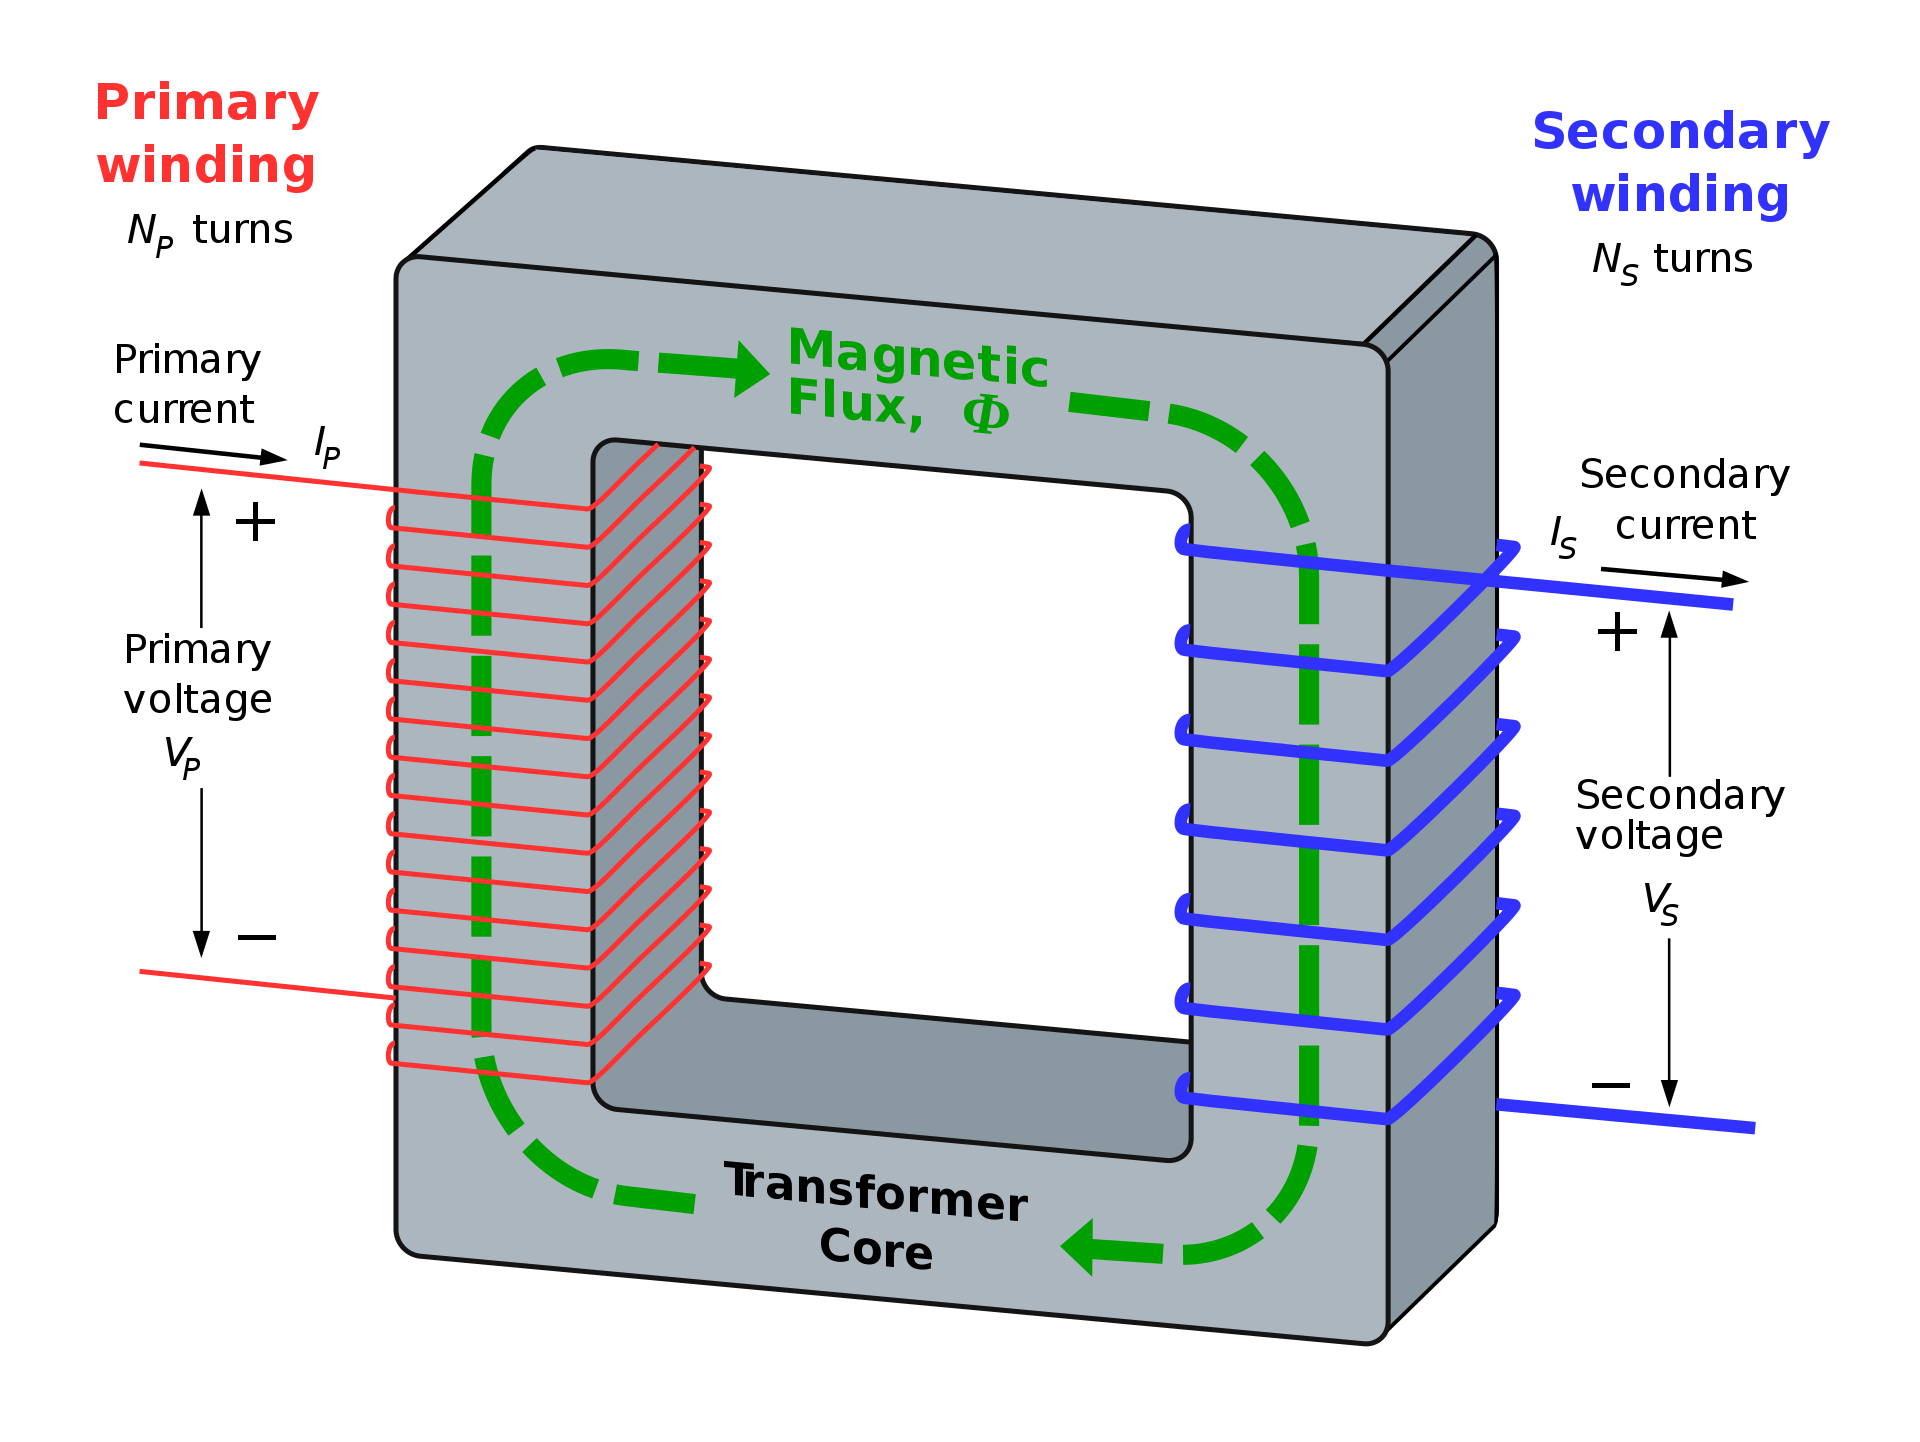
\includegraphics[width=0.8\textwidth]{Trasformatore/trasformatore.png}
\end{figure}

\begin{de}[Trasformatore Ideale Monofase\label{def:trasformatoreIdeale}]
	Il Trasformatore è una macchina elettrica, basata sul fenomeno dell'induzione elettromagnetica, il cui scopo è trasformare tra il circuito primario (ingresso) e il circuito secondario (uscita) la tensione e corrente in ingresso in un altra scala mantenendo inalterata la potenza elettrica.\\
	Permette quindi il trasferimento per mezzo magnetico, di energia tra 2 circuiti fisicamente disaccoppiati, accoppiandoli induttivamente.
	
	In un Trasformatore il circuito Primario e il Secondario condividono lo stesso campo magnetico, e conseguentemente lo stesso flusso $\Phi _{B}$.\\
	Nel caso ideale, quindi, si ha che:
	\begin{vwcol}[widths={0.4,0.6}, sep=8mm, rule=0px]
		\vspace{-3mm}
		\begin{empheq}[box=\mathStep]{equation}
			\Phi_{B} = \Phi_{B_P} - \Phi_{B_S}
		\end{empheq}
		\newpage % con wcol, le colonne sono "pagine"
		\hfill\break \hfill\\[-2mm]\noindent
		{\footnotesize
			Il '$ - $'  tra i campi magnetici è dovuto al verso delle correnti\\
			che creano 2 campi magnetici tra loro contrapposti
		}
	\end{vwcol}
	\noindent
	Siccome tale flusso varia nel tempo, induce nei due avvolgimenti delle f.e.m. (vedi \nameref{def:induttanza}):
	\begin{empheq}[box=\mathStep]{equation}
		e_p = N_1 \frac{d \Phi_{B}}{dt} ; e_s = -N_2 \frac{d \Phi_{B}}{dt}
	\end{empheq}
	I segni non sono entrambi concordi a causa del verso del flusso, che nel primario è concorde e nel secondario discorde (e qui torna la forza di Lenz).\\
	Viste dai morsetti del trasformatore, abbiamo che le tensioni istantanee (dovute alle correnti presenti nei 2 rami) sono pari a:
	\begin{empheq}[box=\mathCalc]{equation} \label{eq:tensioneTrasformatore}
		\displaystyle \left \{ \begin{array}{l}
			V_{P} = R_P I_P + L_{PP} \dot I_P - L_{SP} \dot I_S \\
			V_{S} = R_S I_S - L_{PS} \dot I_P + L_{SS} \dot I_S \\
		\end{array}
		\right.
	\end{empheq}
	Dove $R_P$ e $R_S$ rappresentano le resistenze equivalenti viste dai morsetti (i carichi).\\
	Con i coefficienti di mutua induttanza che si ricavano dalla Def di \nameref{def:induttoreIdeale}:
	
	\begin{center}
		\begin{tabular}[t]{c c}
			$ \displaystyle L_{pp} = \frac{N_P  \Phi_{B_P} }{i_P} $ & $ \displaystyle L_{ps} = \frac{N_S  \Phi_{B_P} }{i_P} $ \\[5mm]
			$ \displaystyle L_{sp} = \frac{N_P  \Phi_{B_S} }{i_S} $ & $ \displaystyle L_{ps} = \frac{N_S  \Phi_{B_S} }{i_S} $
		\end{tabular}
	\end{center}
\end{de}

\noindent
Arrivati a questo punto abbiamo gli strumenti necessari per poter modellare matematicamente l'esperimento in esame nella tesi.
\newpage

\subsection{Modellazione Fisica} \label{subsec:ModelloFisico}
Usando i concetti esposti, vediamo ora una buona approssimazione, passante per un modello lineare a parametri costanti della dinamica tra \textbf{Bobina e Plasma}.\\
Come descritto nell'articolo di \cite{TokamakCircuit}, è possibile modellare la dinamica \textbf{Bobina - Plasma} come fosse il circuito di un
\nameref{def:trasformatoreIdeale}:
\begin{figure}[H]
	\centering
	\caption[Circuito Equivalente Bobina/Plasma all'interno di un Tokamak]{Circuito Equivalente Bobina/Plasma}
	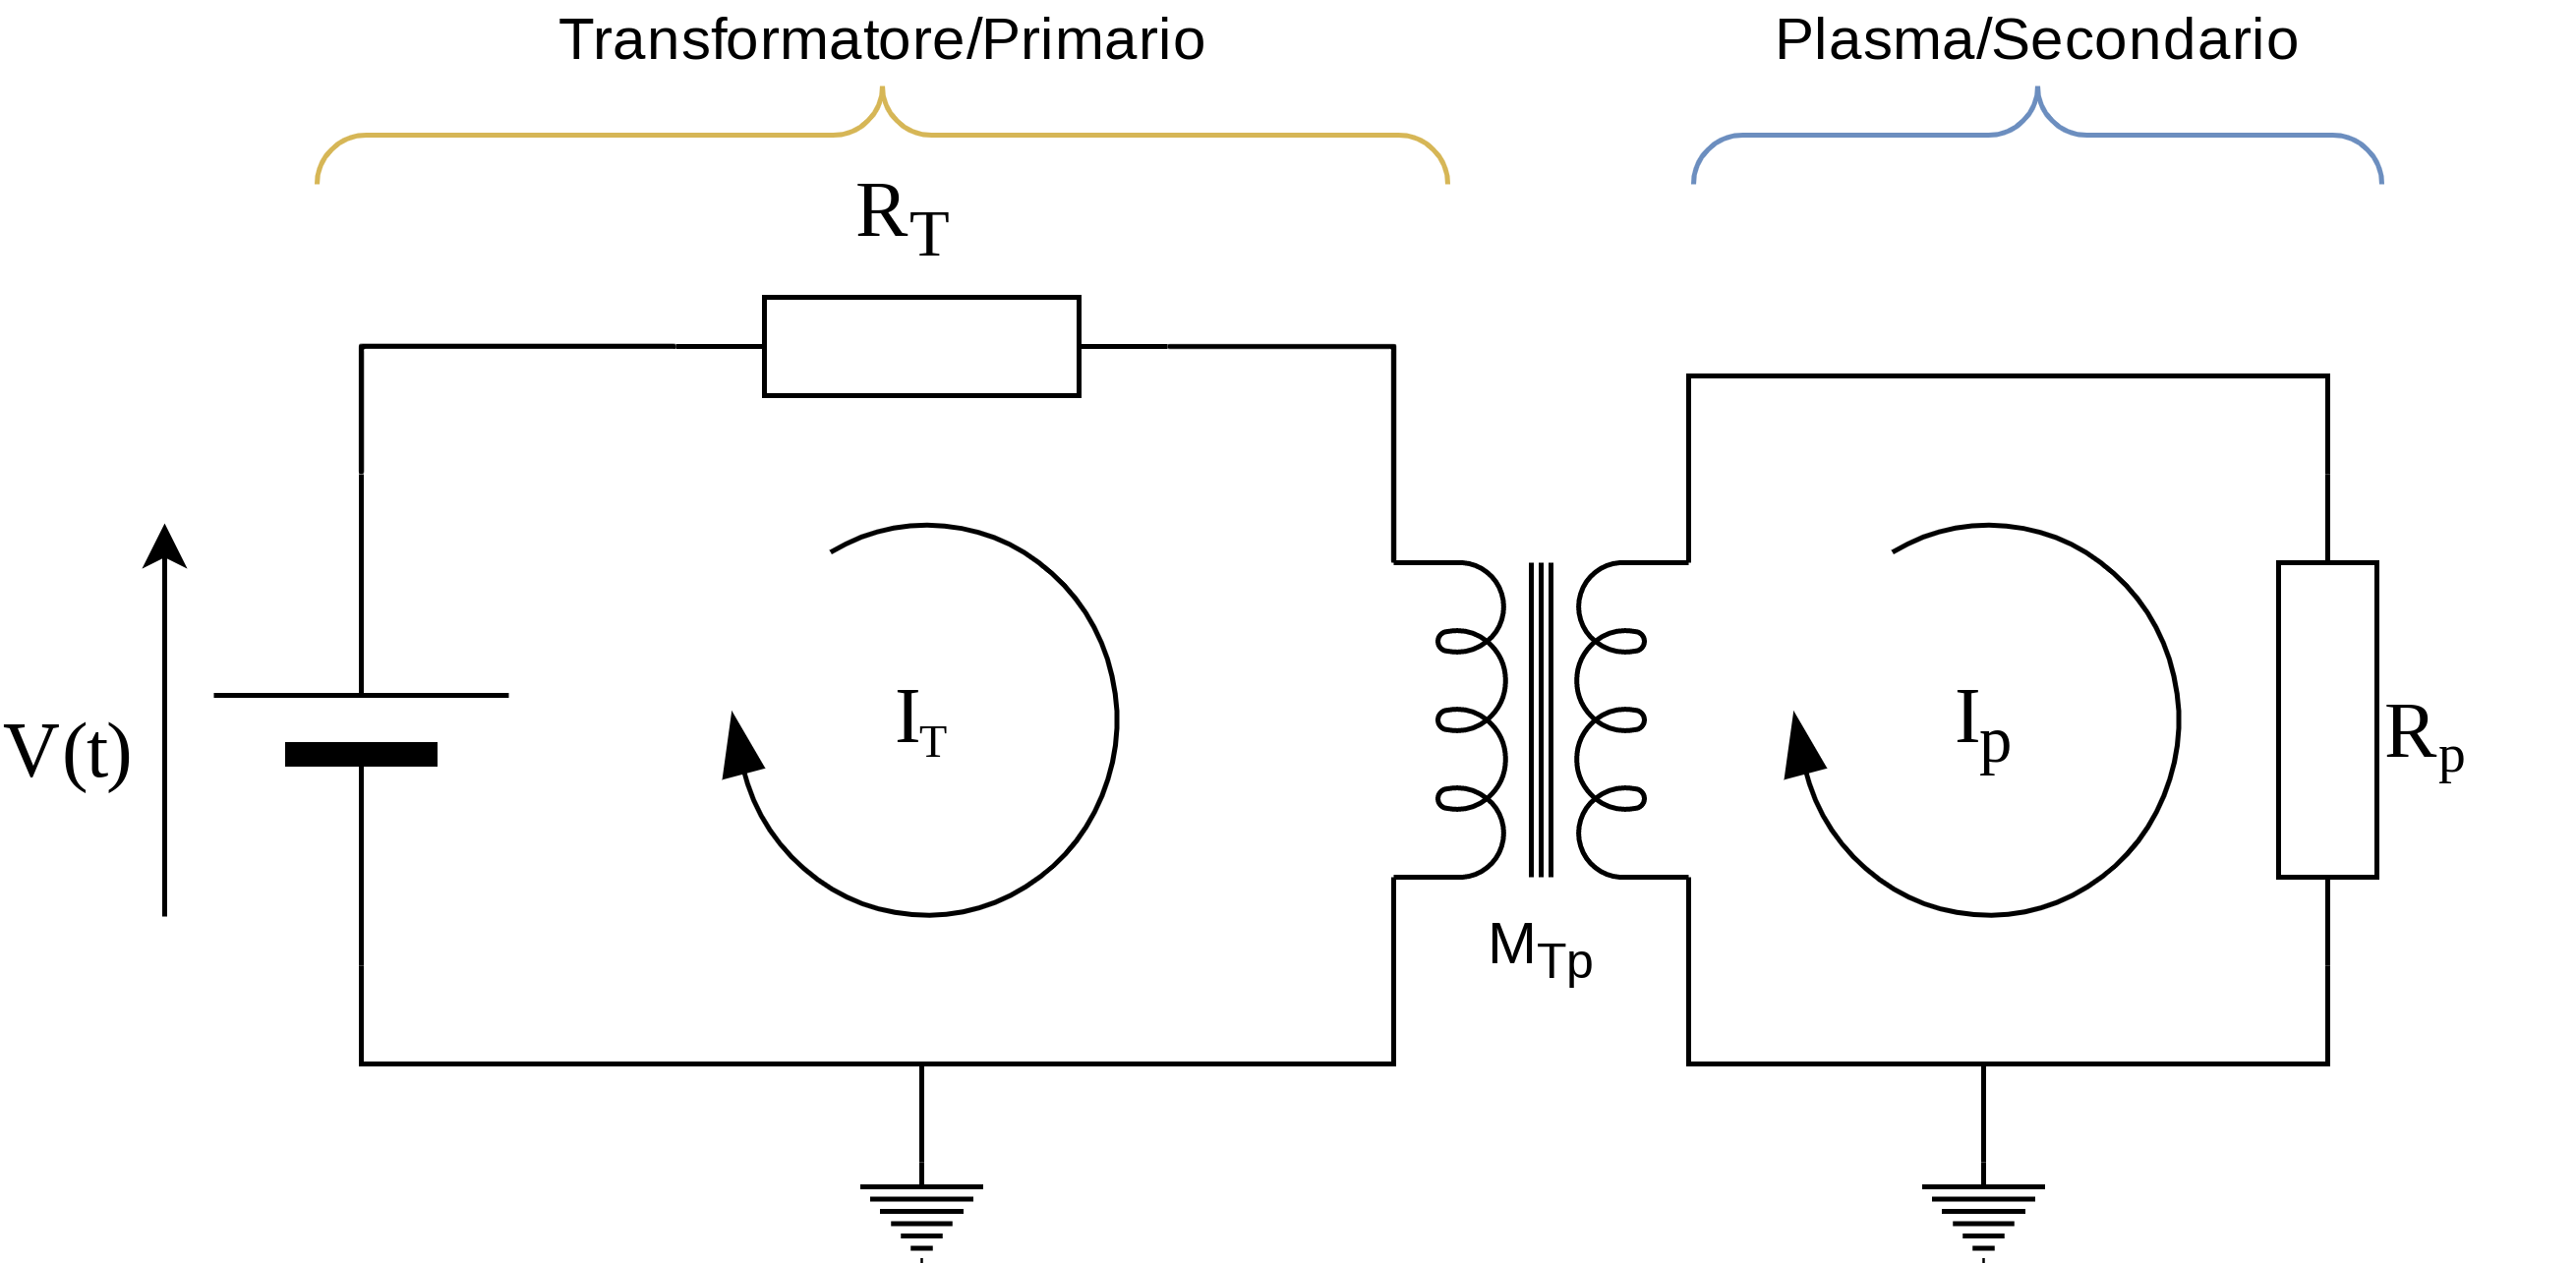
\includegraphics[width=1\textwidth]{Trasformatore/PlasmaCircuit-PlasmaCircuit.png}
\end{figure}
\NumTabs{11}
\begin{leg}
	\item $V(t)$\tab:= Tensione di controllo della Corrente $I_T$
	\item $I_T$\tab:= Corrente del Trasformatore
	\item $R_T$\tab:= Resistenza equivalente Trasformatore
	\item $I_p$\tab:= Corrente di Plasma
	\item $R_p$\tab:= Resistenza di Plasma
	\item $M_{Tp}$\tab:= Coefficiente di Induttanza Trasformatore $\rightarrow$ Plasma
\end{leg}
\paragraph{Difformità dalla realtà} Nella realtà $R_p$ e $M_{Tp}$ sono dei parametri che variano in funzione dello stato del Plasma (Temperatura, Energia, Evoluzione dell'esperimento, ecc\ldots), ma per ovvie ragioni di difficoltà nel riprodurre in laboratorio simili \nonLinearita, noi prenderemo per costanti questi parametri.

\subsection{Semplificazione Primario - Secondario}
Sempre dallo stesso articolo di \cite{TokamakCircuit}, si evince che è possibile modellare questa relazione tra i 2 circuiti prendendo in considerazione \textbf{solo} le forze di induzione dovute alla corrente che il Primario trasferisce sul Secondario, ciò permette di semplificare ulteriormente il circuito trascurando le correnti indotte dal Plasma dentro la Bobina del Primario.\\
Usando queste osservazioni si ottiene quindi il circuito equivalente:
\begin{figure}[H]	\label{fig:PlasmaSemplificato}
	\centering
	\caption[Circuito Semplificato Bobina/Plasma]{Circuito equivalente Bobina/Plasma semplificato}
	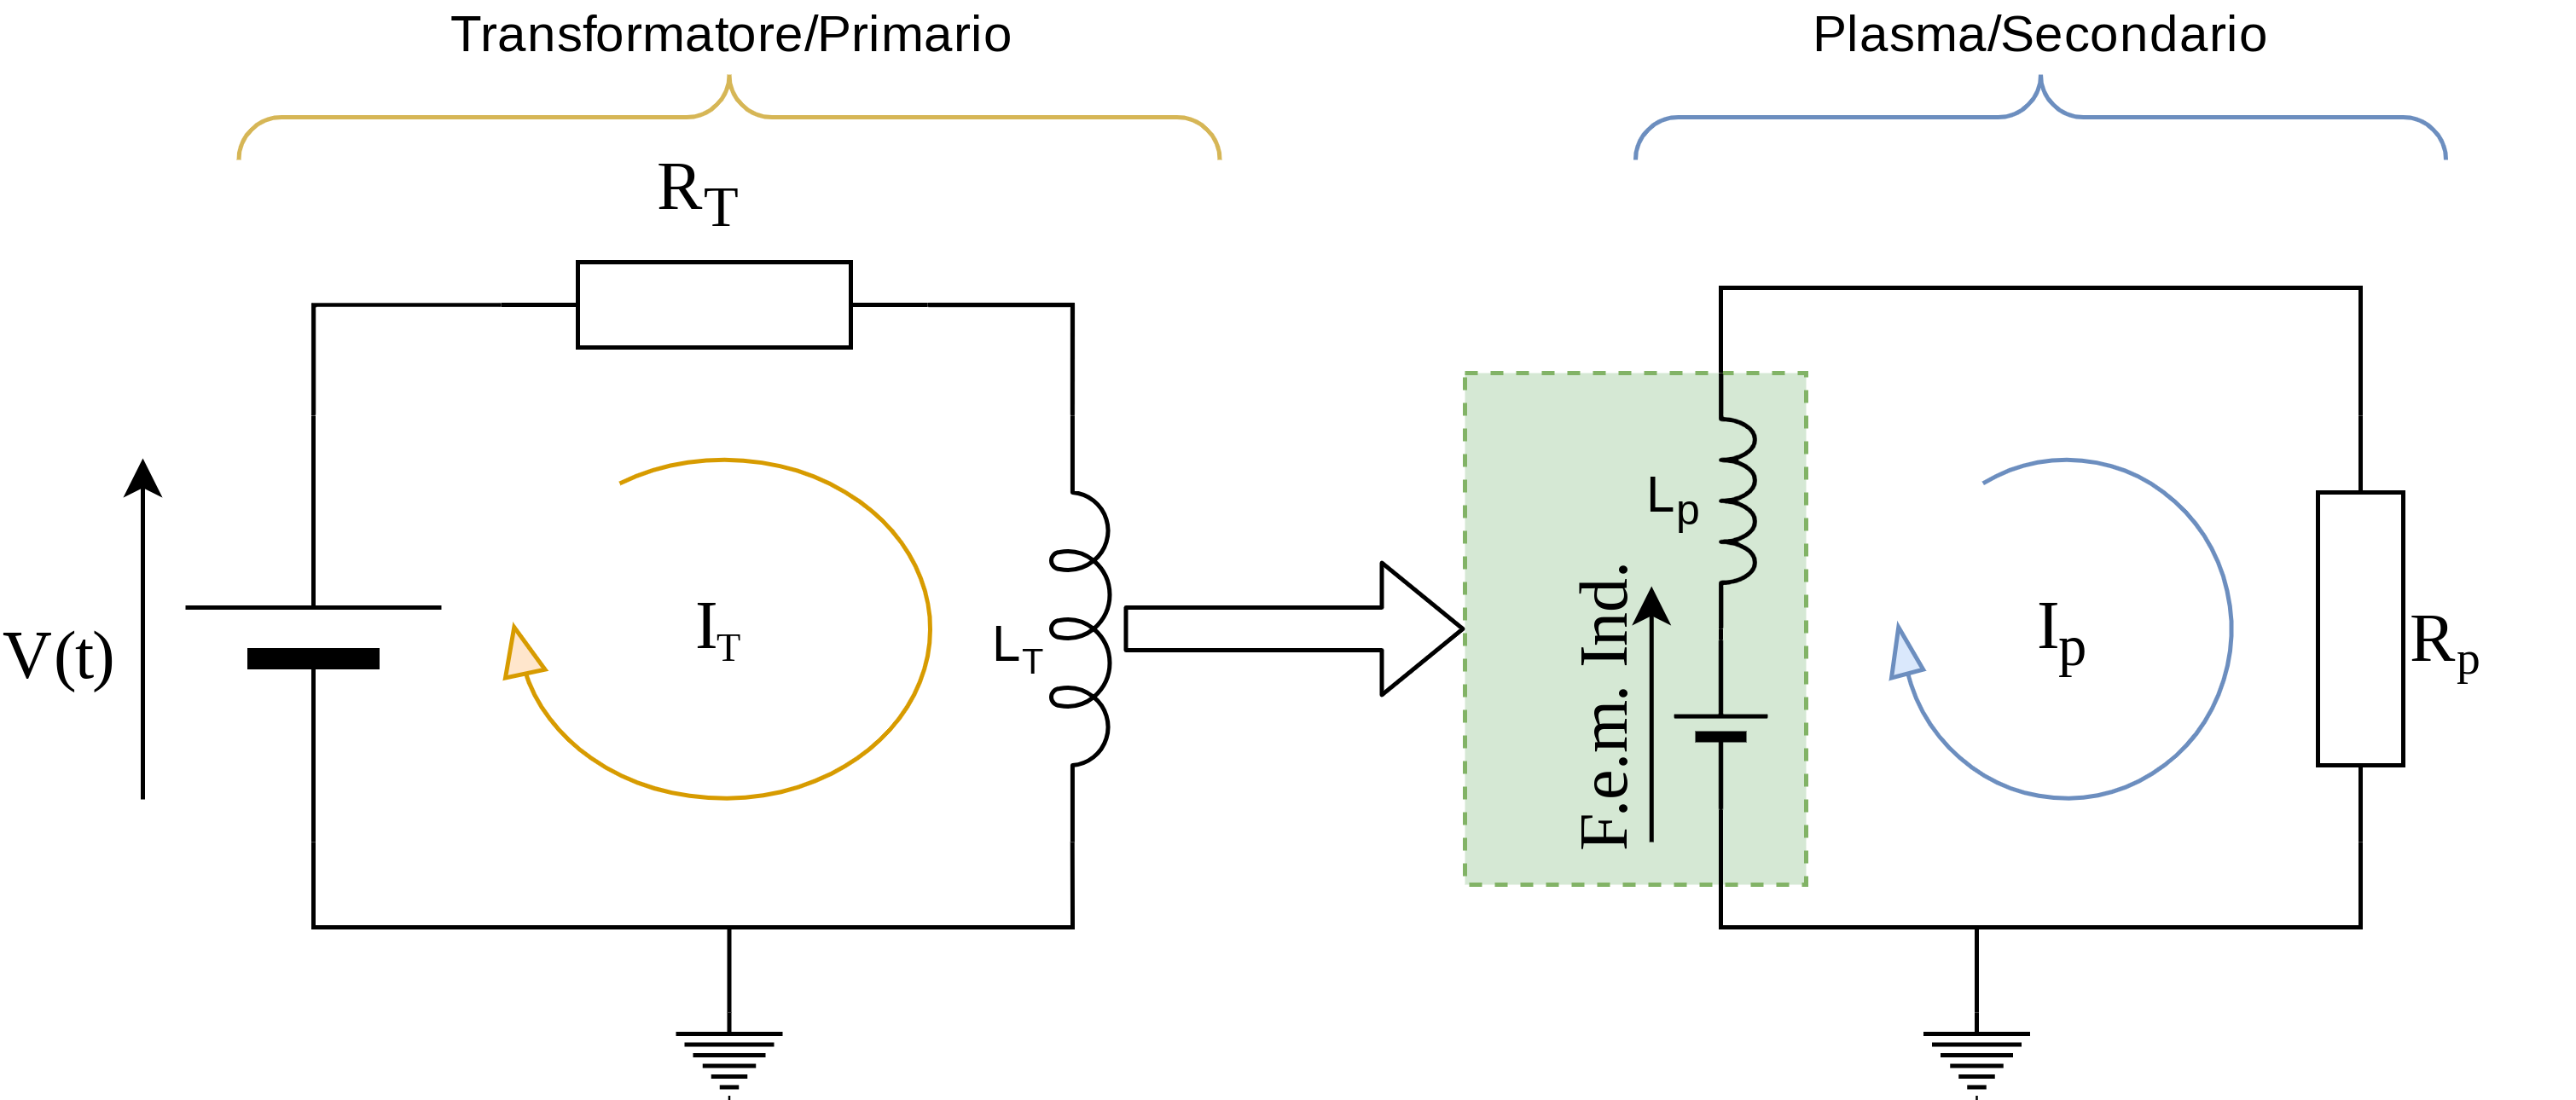
\includegraphics[width=1\textwidth]{Trasformatore/PlasmaCircuit-EquivalentCalc.png}
\end{figure}

\NumTabs{11}
\begin{leg}
	\item $V(t)$\tab:= Tensione di controllo della corrente $I_T$
	\item $I_T$\tab:= Corrente del Trasformatore
	\item $R_T$\tab:= Resistenza equivalente Trasformatore
	\item $I_p$\tab:= Corrente di Plasma
	\item $R_p$\tab:= Resistenza di Plasma
	\item $M_{Tp}$\tab:= Coefficiente di Induttanza Trasformatore $\rightarrow$ Plasma
	\begin{itemize} [topsep=-1mm,itemsep=0mm,label=$ \circ $]
		\item $L_T$\tab:= Induttanza equivalente Trasformatore
		\item $L_p$\tab:= Induttanza equivalente Plasma
	\end{itemize}
\end{leg}
\noindent
Usando questa semplificazione dall'equazione \ref{eq:tensioneTrasformatore} del trasformatore ignoriamo che la tensione sul Primario è influenzata dal Secondario; in questa condizione il circuito del Primario evolve come sistema indipendente rispetto al Secondario, e la sua evoluzione influenza il Secondario senza risentirne.

\newpage
\subsection{Dal circuito alla dinamica}\label{subsec:dinamicaCircuito}
Analizziamo ora la dinamica del circuito semplificato \ref{fig:PlasmaSemplificato} analizzando le 2 maglie del circuito:
\subsubsection{Dinamica di Plasma}
\vspace{-2mm}
Per calcolare la dinamica della corrente di Plasma usando la \nameref{th:KirchhoffMaglie} sulla maglia del secondario:
\begin{empheq}[box=\mathStep]{equation*}
	F_{em} = L_p \dot I_p + I_p R_p
\end{empheq}
Grazie al principio dell'\nameref{def:induttanza} siamo in grado di risalire al termine generatrice della $F_{em}$: 
\begin{empheq}[box=\mathStep]{equation*}
	F_{em} = -M_{Tp} \dot I_T
\end{empheq}
Perciò, unendo insieme i blocchi otteniamo:
\begin{vwcol}[widths={0.6,0.4}, sep=5mm, rule=0px]
	\vspace{-3mm}
	\begin{empheq}[box=\mathCalc]{equation} \label{eq:correntePlasmaDinamica}
		-M_{Tp} \dot I_T = L_p \dot I_p + I_p R_p
	\end{empheq}
	\newpage % con wcol, le colonne sono "pagine"
	\hfill\\[-1mm]\noindent
	\begin{spacing}{1.25}
		{\footnotesize
			Da notare la somiglianza con\\
			l'equazione del trasformatore \ref{eq:tensioneTrasformatore}
		}
	\end{spacing}
\end{vwcol}\vspace{-3mm}
\noindent
\begin{oss}
	Dalla eq \ref{eq:correntePlasmaDinamica} è interessante notare che rendere la corrente di Plasma costante, equivale a fissare una $F_{em}$ di costante.\\
	In un Tokamak reale, anche se l'obiettivo è controllare la corrente di Plasma, misurarla direttamente risulta essere problematico, a tale scopo nei Tokamak reali, viene usata la \textbf{Tensione di Loop} (\cite{MagneticDiagnostics}) come indicatore della $ I_p $, che nel nostro caso coincide esattamente con la $ F_{em} $ del secondario (problematica discussa in seguito, vedi \nameref{sub:parametriMisurati}).
\end{oss}


\subsubsection{Dinamica del Trasformatore}
\vspace{-3mm}
Vediamo ora la dinamica della corrente del Trasformatore, in funzione della \textit{Tensione di controllo}.\\
Il calcolo avviene seguendo gli stessi procedimenti della corrente di Plasma, usando sempre il \nameref{th:KirchhoffMaglie}, e si ottiene come equazione di maglia:
\begin{empheq}[box=\mathCalc]{equation} \label{eq:correnteTrasformatoreDinamica}
	V(t) = L_T \dot I_T + I_T R_T
\end{empheq}

\subsection{Funzione di Trasferimento}
Nella sezione "\nameref{subsec:dinamicaCircuito}" abbiamo ottenuto la dinamica istantanea dei 2 rami del circuito \ref{fig:PlasmaSemplificato}.\\
Vogliamo ora ricavare le funzioni di trasferimento dei 2 rami e trovare così la funzione di trasferimento Ingresso uscita del Trasformatore.
\subsubsection{Funzione di Trasferimento Plasma}
\vspace{-3mm}
Volendo calcolare la funzione di trasferimento per le dinamiche forzate, partiamo dall'equazione \ref{eq:correntePlasmaDinamica} risolvendola per condizioni iniziali nulle.
\begin{center}
	{\large
		$ s I_p L_p  + I_p R_p = -s I_T M_{Tp} \Rightarrow I_p( s L_p + R_p) = -s I_T M_{Tp} \Rightarrow$ \\ 
		$ I_p(s) = \frac{-s M_{Tp}}{ s L_p + R_p} I_T(s) $
	}
\end{center}
\noindent
Arrivando così a scrivere come funzione di trasferimento per il Plasma (Secondario):
\begin{empheq}[box=\mathCalc]{equation} \label{eq:correntePlasmaLaplace}
	\frac{I_p(s)}{I_T(s)}  = \frac{-s M_{Tp}}{ s L_p + R_p}
\end{empheq}

\subsubsection{Funzione di Trasferimento Trasformatore}
\vspace{-5mm}
Similmente a quanto fatto per Plasma, partendo dall'equazione \ref{eq:correnteTrasformatoreDinamica} in condizioni iniziali nulle abbiamo:
\begin{center}
	{\large
		$ s I_T L_T  + I_T R_T = V(s) \Rightarrow I_T( s L_T + R_T) = V(s) \Rightarrow $\\
		$ I_T(s) = \frac{1}{s L_T + R_T} V(s)$
	}
\end{center}
\noindent
Ottenendo così la funzione di trasferimento del Trasformatore (Primario):
\begin{empheq}[box=\mathCalc]{equation} \label{eq:correnteTrasformatoreLaplace}
	\frac{I_T(s)}{V(s)}  = \frac{1}{s L_T + R_T}
\end{empheq}
\newpage
\begin{oss} \label{oss:Iref}
	La funzione di trasferimento che abbiamo ottenuto rispecchia il circuito dell'esperimento lasciandoci come variabile di controllo la $ V(t) $.\\
	A livello teorico però, noi controlliamo la corrente sul primario e puntiamo a osservare una corrente sul secondario,abbiamo quindi un sistema che si controlla in corrente e che ha un uscita in corrente.\\
	Sarebbe quindi utile e opportuno allora riassegnare l'ingresso di tensione mettendo in evidenza la variabile virtuale $ I_{ref} $:
	\begin{empheq}[box=\mathStep]{equation*}
		V(t)=I_{ref}(t) \cdot R_T \Rightarrow I_{ref}(t) = \frac{V(t)}{R_T}
	\end{empheq}
	Ottenendo quindi come funzione di trasferimento del Trasformatore (Primario): 
	\begin{empheq}[box=\mathCalc]{equation}
		I_T(s) = \frac{R_T}{(s L_T + R_T)} I_{ref}(s) = \frac{1}{(s \frac{L_T}{R_T} + 1)} I_{ref}(t)
	\end{empheq}
	In questa forma possiamo osservare che, per $I_{ref}(t)=I_{ref}$ costante, superato il transitorio, si ottiene $I_T = I_{ref}$, da cui abbiamo che la corrente sul trasformatore viene attuata con un certo ritardo dovuto alla costante di tempo $\tau = \frac{L_T}{R_T}$
\end{oss}

\subsubsection{Funzione di Trasferimento Complessiva}\label{subsubsec:FuncTrasfImpianto}
\vspace{-5mm}
Connettendo in serie i 2 blocchi e tenendo conto dell'osservazione \ref{oss:Iref} si ottiene:
%\vspace{-3mm}
\begin{empheq}[box=\mathCalc]{equation} \label{eq:FuncTrasfTot}
	P(s) = \frac{I_p(s)}{I_{ref}(s)} = \frac{I_T(s)}{I_{ref}(s)} \cdot \frac{I_p(s)}{I_T(s)}  = -\frac{s M_{Tp}}{( s L_p + R_p)(s L_T + R_T)}
\end{empheq}

\noindent
Che vista come schema a blocchi diventa:\vspace{-2mm}
\begin{figure}[H]
	\centering
	\caption[Schema a Blocchi della funzione di trasferimento della corrente di Plasma]{Schema a Blocchi Corrente di Plasma}
	\vspace{2mm}
	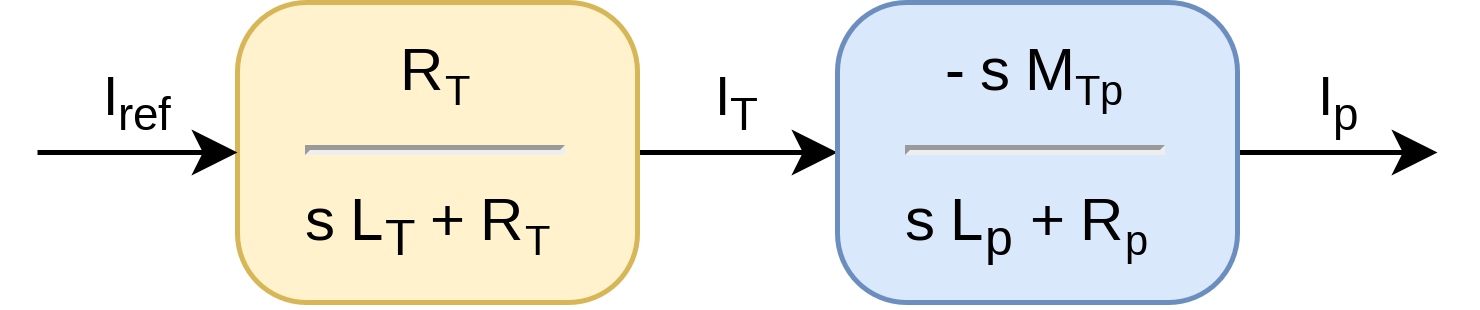
\includegraphics[width=1\textwidth]{Trasformatore/PlasmaCircuit-SchemaBlocchi.png}
\end{figure}\vspace{-6mm}
\noindent
Essendo il segno di uscita del segnale inverso rispetto al segnale d'ingresso, eliminiamo questo fastidio aggiungendo matematicamente un '$ - $' e a livello di prototipo invertendo i fili sul Secondario. Così facendo otteniamo come funzione di trasferimento complessiva:
\begin{empheq}[box=\mathCalc]{equation} \label{eq:FuncTrasfTotPos}
	P_{pos}(s) = -P(s) = \frac{s M_{Tp}}{( s L_p + R_p)(s L_T + R_T)} = \frac{-I_p(s)}{I_{ref}(s)}
\end{empheq}

\subsection{Misura del campo Elettrico del Plasma come indice per la Corrente} \label{sub:parametriMisurati}
Riprendendo l'equazione della corrente di Plasma \ref{eq:correntePlasmaDinamica}, abbiamo che il campo elettrico indotto sul Plasma, ovvero la $F_{em}$, dipende direttamente dallo stato della corrente di Plasma $I_p$.\\
Da essa abbiamo che per $I_p$ costanti, anche la $F_{em}$ è costante.\\
Nel caso del trasformatore si potrebbe fisicamente misurare la corrente di Plasma, simulata dalla corrente sul secondario, ma nel caso di un impianto reale, risulta evidente che è impossibile.\\
Proprio per questo, come descritto da \cite{MagneticDiagnostics},a pagina 12, si usa come indice di misura Tensione di giro $V_{loop}$ ($\Rightarrow F_{em}$ nel nostro esperimento).\\
Perciò il circuito reale usato nell'esperimento della tesi, comprensivo di misure è:
\begin{figure}[H] \label{fig:circuitoDiMisura}
	\centering
	\caption[Circuito reale di misura dell'esperimento]{Circuito di misura}
	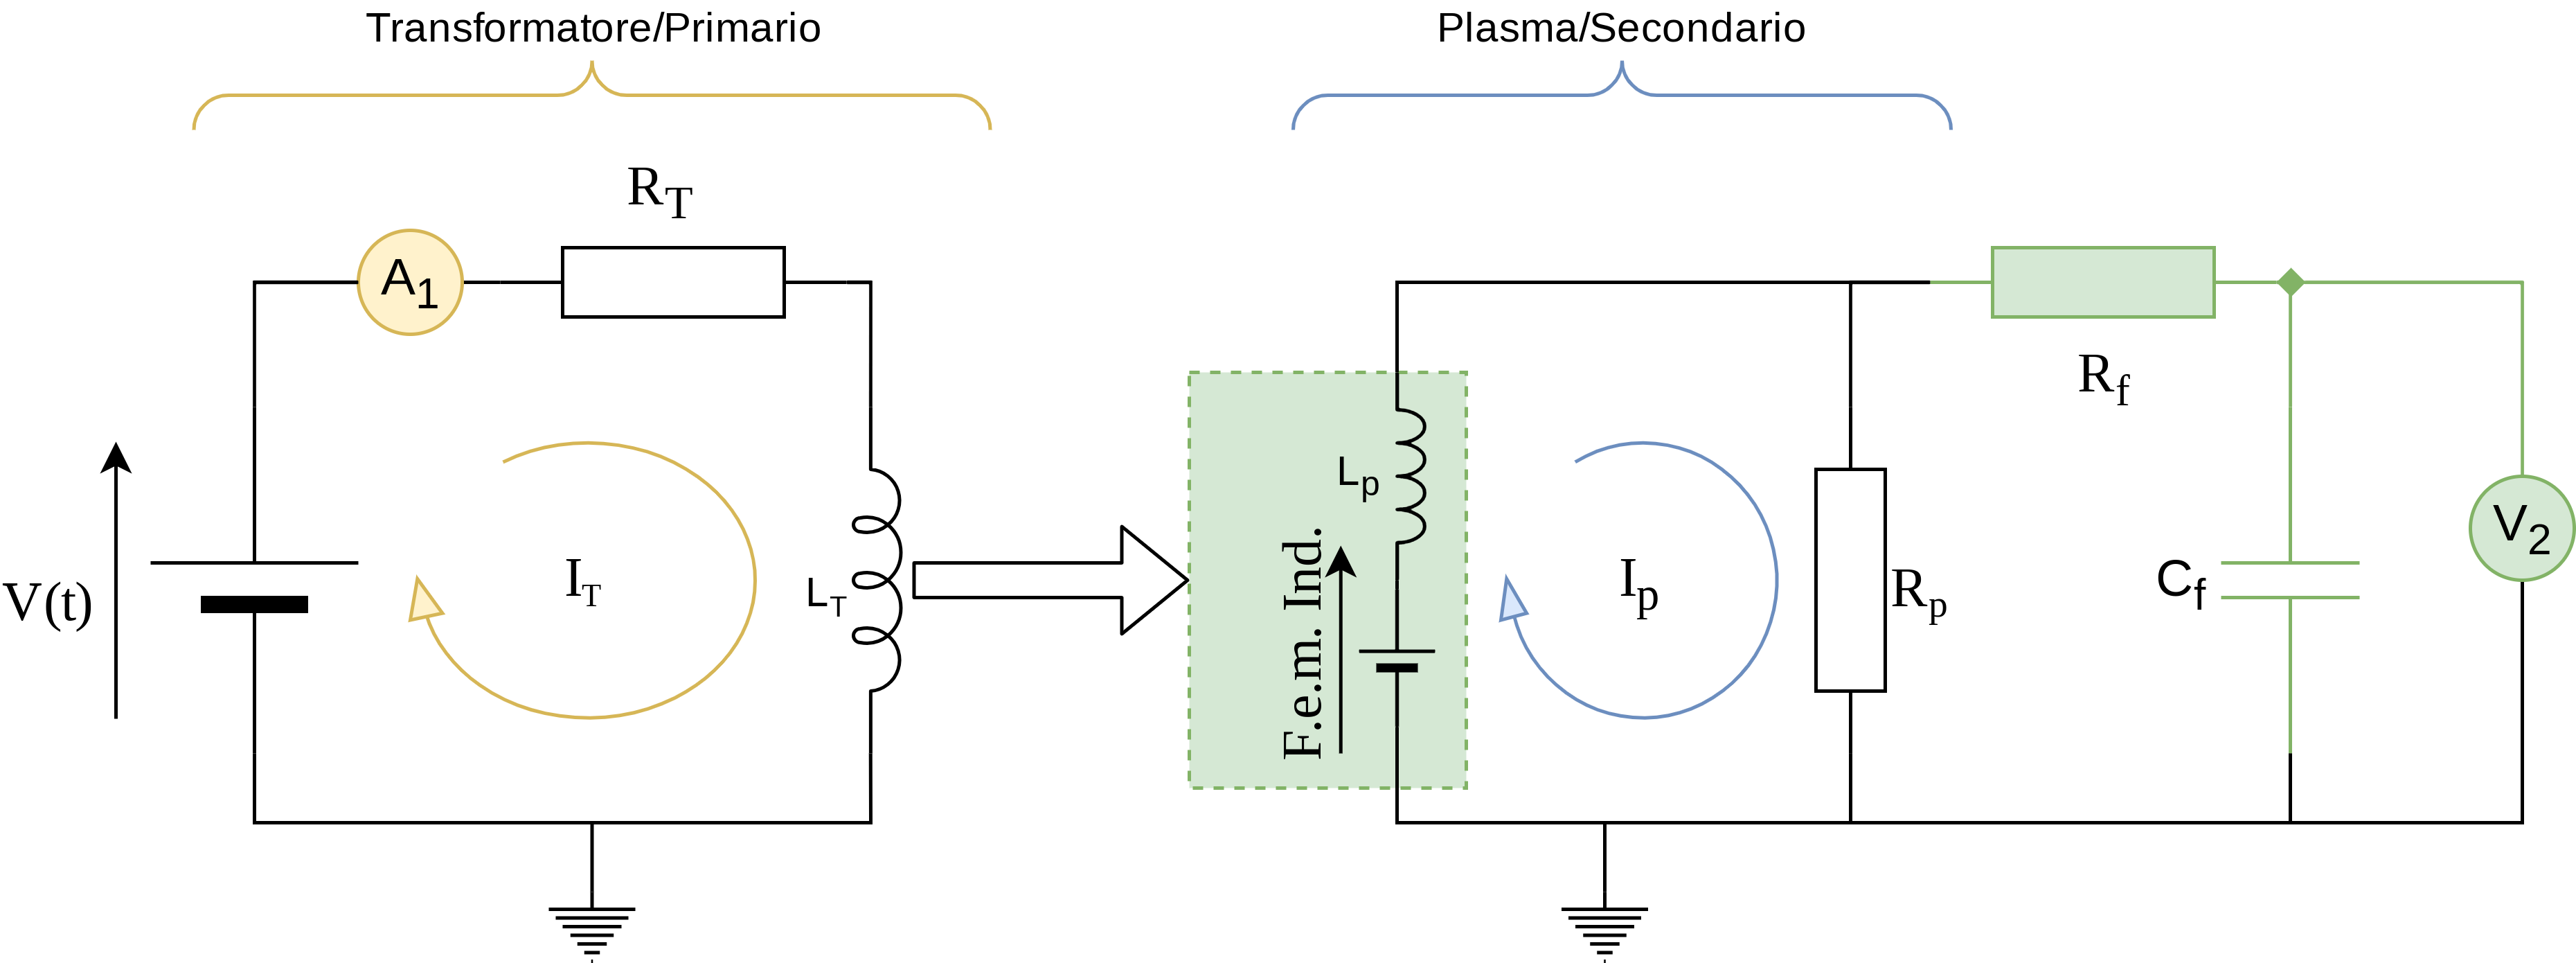
\includegraphics[width=1\textwidth]{Trasformatore/PlasmaCircuit-MisureCircuit.png}
\end{figure}

Abbiamo quindi, tra ingresso e uscite i parametri di:
\begin{itemize}
	\item $I_T$ misurata dal sensore di corrente $ A_1 $ \nameref{CurrentSense}.
	\item $F_{em}$ misura dal voltmetro $V_2$ (che è realizzata da un Pin analogico del \microControllore) e che rappresenta un indice per  la corrente $I_p$ quando essa è costante (eq \ref{eq:correntePlasmaDinamica}).
	\item $V(t)$ generata in base alla legge di controllo, e attuata mediante PWM (\cite{modulazionePWM}) dal driver di corrente \nameref{CurrentDriver}.
\end{itemize}


\newpage


\section{Trasduttore di Corrente}\label{CurrentSense}
Come già discusso precedentemente, l'obiettivo della tesi è di controllare la corrente sul secondario. In tale ottica la misura della corrente sul Primario potrebbe non essere una misura di interesse. Essendo però un lavoro di ricerca, si è preferito poter misurare la corrente effettivamente circolante nel Primario del trasformatore, così da poter meglio interpretare i dati misurati senza ambiguità.
\begin{figure}[H]
	\centering
	\caption[Sensore di Corrente \citefield{ACS770}{series}]{Sensore di Corrente}
	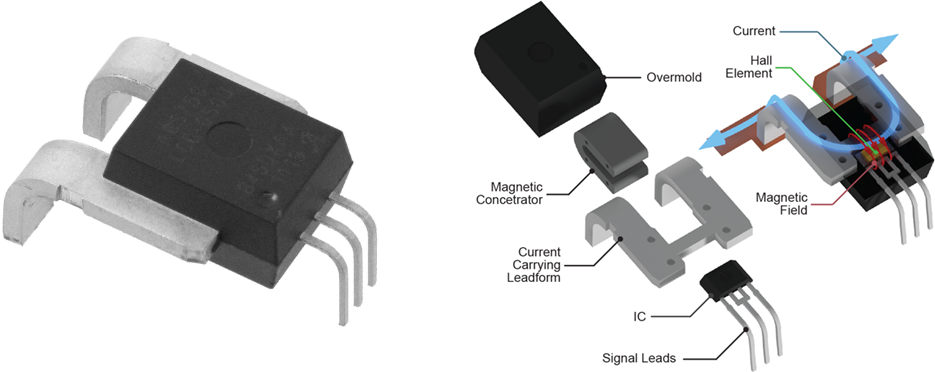
\includegraphics[width=1\textwidth]{ACS770/ACS770-Fig.png}
\end{figure}
%\vspace{-1cm}
\subsection{Sensore scelto}
Per misurare la corrente del primario, si è usato il sensore di Corrente \cite{ACS770}. La famiglia di sensori ha in generale le seguenti caratteristiche:
\begin{table}[H]
	\centering
	\label{tab:ACS770ParametriGenerali}
	\caption[\cite{ACS770}  Riassunto caratteristiche]{Riassunto caratteristiche}
	\begin{tabular}[t]{|l r|}
		\hline
		Bandwidth:                             & 120 kHz                               \\
		Output rise time :                     & 4.1 $ \mu s $                         \\
		Ultralow power loss:                   & 100 $ \mu \Omega $ Resistenza Interna \\
		Single supply operation                & 4.5 to 5.5 V                          \\
		Extremely stable output offset voltage &                                       \\
		\hline
	\end{tabular}
\end{table}
\noindent
In oltre, delle tante varianti esistenti, si è scelto di usare la \citefield{ACS770}{series}, le cui caratteristiche chiave sono:

\begin{table}[H]
	\centering
	\label{tab:ACS770ParametriParticolari}
	\caption[\citefield{ACS770}{series} Particolarità]{\citefield{ACS770}{series} Particolarità}
	\begin{tabular}[t]{|l r|}
		\hline
		Primary Sampled Current: & $\pm$ 100 A     \\
		Sensitivity Sens (Typ.)  & 20(mV/A)        \\
		Current Directionality   & Bidirectional   \\
		$T_{OP}$                 & –40 to 150 (°C) \\
		\hline
	\end{tabular}
	
\end{table}
\noindent
Le caratteristiche più importanti di questo trasduttore sono l'ampio margine di misura, e la robustezza alle variazioni di temperatura, che insieme rendono il dispositivo perfetto per misurare le energie dei nostri esperimenti attuali, e lo rendono \textit{future-proof} per esperimenti futuri quando si useranno energie superiori.

\subsection{Criticità}
Unico punto dolente, ma comune al tutti i sensori a effetto induttivo, è proprio il suo principio di funzionamento: essendo il sensore basato su un l'effetto Hall, ovvero una misura diretta del campo magnetico indotto dalla corrente nel conduttore, lo rende soggetto alle variazioni di campo magnetico prodotte propri dal Trasformatore Centrale, che nei suoi momenti di massimo flusso, genera ovviamente un campo magnetico non indifferente.
\begin{figure}[H]
	\centering
	\caption[Metodo di misura di corrente mediante effetto Hall]{Misura di corrente per effetto Hall}
	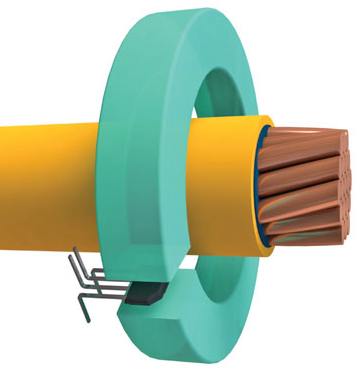
\includegraphics[width=0.5\textwidth]{ACS770/effettoHall.png}
\end{figure}
\newpage
\subsection{Funzionamento Interno}
\vspace{-5mm}
\begin{figure}[H]
	\centering
	\caption[\citefield{ACS770}{series} Schema a Blocchi]{Schema a Blocchi}
	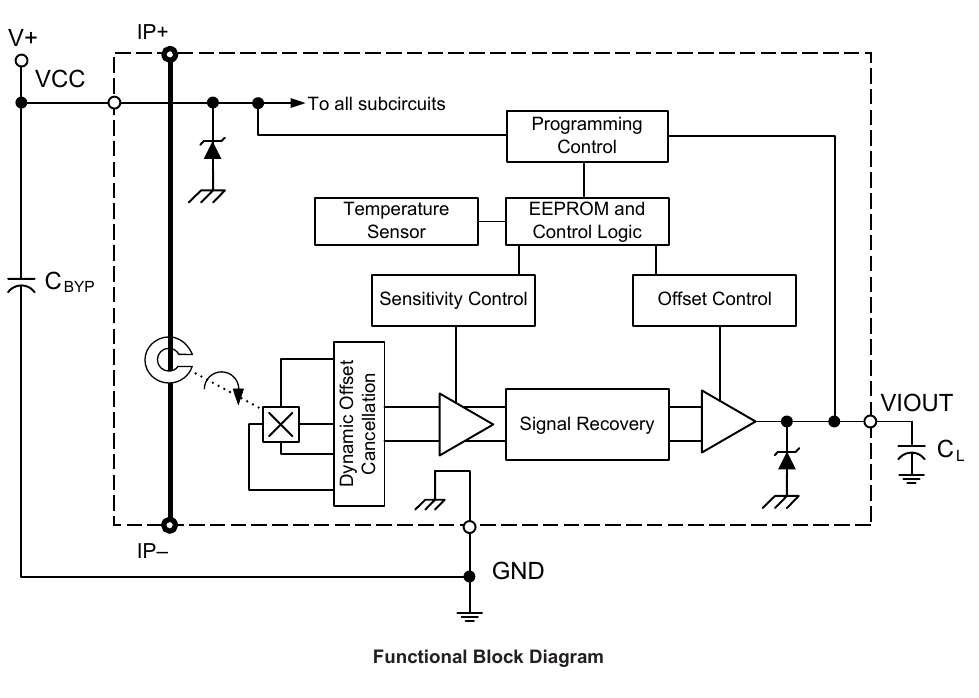
\includegraphics[width=1\textwidth]{ACS770/ACS770-SchemaBlocchi.png}
\end{figure}
\noindent
Tra le caratteristiche chiave dell'\cite{ACS770}, troviamo il disaccoppiamento fisico tra la corrente da misurare e il circuito di misura (ben visibile nello schema a blocchi). Questa caratteristica chiave, garantisce la salvaguardia del circuito logico a valle, dai possibili eventi catastrofici a monte.\\
Esso è in oltre fornito di sensori di temperatura e sistemi di \textit{Signal Recovery} che permettono all'Hardware stesso di compensare parzialmente \nonLinearita termiche della misura per effetto Hall, ottenendo un output assimilabile a un segnale lineare:
\newpage
\begin{figure}[H]
	\centering
	\caption[\citefield{ACS770}{series} Sensibilità rispetto Temperatura]{Sensibilità}
	\includegraphics[width=0.65\textwidth]{ACS770/ACS770-Sensibilità.png}
\end{figure}
\vspace{-5mm}
\noindent
Come si può vedere dal grafico, gli errori sono tanto più marcati quanto maggiore è la corrente da misurare ed in oltre questo errore ha una forte dipendenza dalla temperature dell'esperimento:\\\vspace{-12mm}
\begin{figure}[H]
	\centering
	\caption[\citefield{ACS770}{series} \nonLinearita]{Temperatura/NonLinearità}
	\vspace{1mm}
	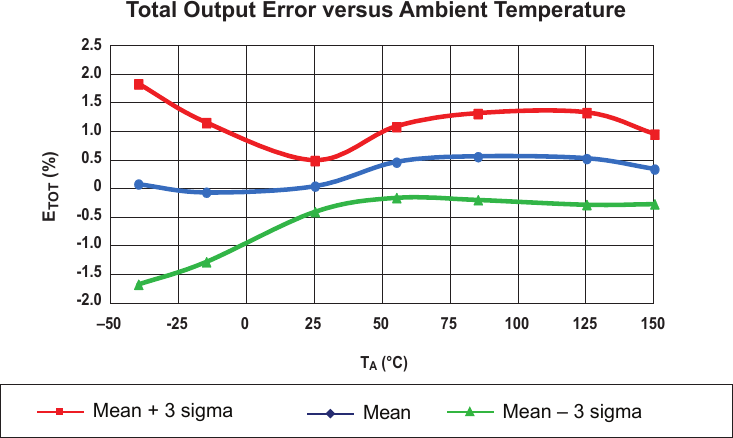
\includegraphics[width=0.9\textwidth]{ACS770/ACS770-NonLin.png}
\end{figure}\vspace{-6mm}

\noindent
Il quale però non è mai, neanche negli esperimenti più sfortunati, superiore al $\pm2\%$.\\
Anzi, alle temperature $\approx$ 25°, si mantiene contenuto tra $\pm0.5\%$.

\newpage

\subsection{Connessione elettrica}

La connessione del sensore è particolarmente semplice, richiedendo esternamente solo un alimentazione stabilizzata e portando subito in uscita la misura di corrente sotto forma di tensione.
\begin{figure}[H]
	\centering
	\caption[\citefield{ACS770}{series} Schema di collegamento dal Datasheet]{Collegamento dal Datasheet}
	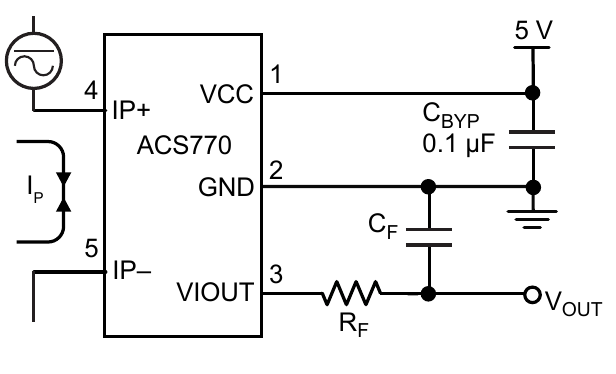
\includegraphics[width=0.85\textwidth]{ACS770/ACS770-Schema.png}
\end{figure} \vspace{-8mm}
\noindent
Rispetto allo schema proposto dal datasheet, però, si è deciso di omettere il filtro passa-basso sulla \textbf{VIOUT}, questa scelta è stata presa per minimizzare il più possibile ritardi di misura della corrente istantanea desiderabile poiché le dinamiche del sistema sul secondario, come visto, sono di tipo derivativo, e quindi estremamente rapide.\\
Questa scelta è stato possibile prenderla poiché la corrente per alimentare l'esperimento proviene da una batteria con un alta capacità di scarica istantanea (fino a 1000A), da cui l'assenza di disturbi sul segnale di corrente e la possibilità di prendere questa scelta.

\subsection{Dalla misura alla corrente}
Il trasduttore è basato sull'effetto Hall, il quale permette di misurare una corrente attraverso il campo magnetico che crea, e riporta questa misura sotto sotto forma di tensione.\\
I sensori della famiglia \cite{ACS770} propongono vari modelli che differiscono tra loro principalmente per la \textbf{Sensibilità} di misura e la lettura di corrente \textit{Bi-direzionale} o \textit{Mono-direzionale} , in funzione della scala di misura che si vuole avere e della presenza di corrente alternata o continua.
Per i nostri scopi abbiamo preso il modello: '\citefield{ACS770}{series}', di cui i parametri sono riportati in tabella \ref{tab:ACS770ParametriParticolari}.\\
Usando la sensibilità riportata in tabella, abbiamo che la formula di conversione per ottenere la corrente letta è:
 \begin{center}
 	{\large $I_{read} = \frac{V_{Read}[V]}{V_{sense}[V/A]}$ }
\end{center}


\paragraph{Rimozione Offset}
Essendo però l'ACS770 ad alimentazione singola (0--5V), ma la corrente misurabile \textbf{Bi-Direzionale}, sorge la necessità di spostare il riferimento della corrente nulla ad una tensione superiore allo 0V.\\
Il datasheet riporta che $V_{offset} = \frac{Vcc}{2}\approx$ 2.5V. Da cui deriva che la vera misura di corrente è:

{\large
\begin{empheq}[box=\mathCalc]{equation}\label{eq:Iread}
	I_{read} = \frac{V_{Read}-V_{offset}}{V_{sense}} \frac{[V]}{[V/A]}
\end{empheq}
}
\noindent
Al fine di poter misurare l'offset effettivo, durante il set-up viene eseguito a esperimento fermo una misura dell'offset attuale, usando la \nameref{lst:offsetCalc}.\\
Il risultato della computazione, oltre ad essere usato nel controllo è inviato al computer per la post elaborazione dei dati nei grafici.

\paragraph{Analisi Sensibilità}
Usando nell'esperimento un ADC a 10Bit con tensione di riferimento a 5V, abbiamo che la massima sensibilità del \microC, ovvero il suo bit meno significativo è pari a:
%\vspace{-5mm}
\begin{empheq}[box=\mathResult]{equation} \label{result:Vstep}
	V_{step}=\frac{Vcc}{2^{10}-1} = 4,887mV
\end{empheq}
\noindent
Il che equivale a una \textbf{Sensibilità di Corrente} del $\mu$Controllore pari a:
%\vspace{-5mm}
\begin{empheq}[box=\mathResult]{equation} \label{result:Istep}
	I_{step} =\frac{ V_{step}}{V_{sense}} = 244,379 mA
\end{empheq}

\newpage

\section{Driver di Corrente - IBT-2}\label{CurrentDriver}
Per l'attuazione del controllo di corrente nella bobina primaria del trasformatore, è stato usato il driver di corrente \cite{IBT-2} .


\begin{figure}[H]
	\centering
	\caption[Driver Motori IBT-2 TopView \& PinOut]{IBT-2 TopView.}
	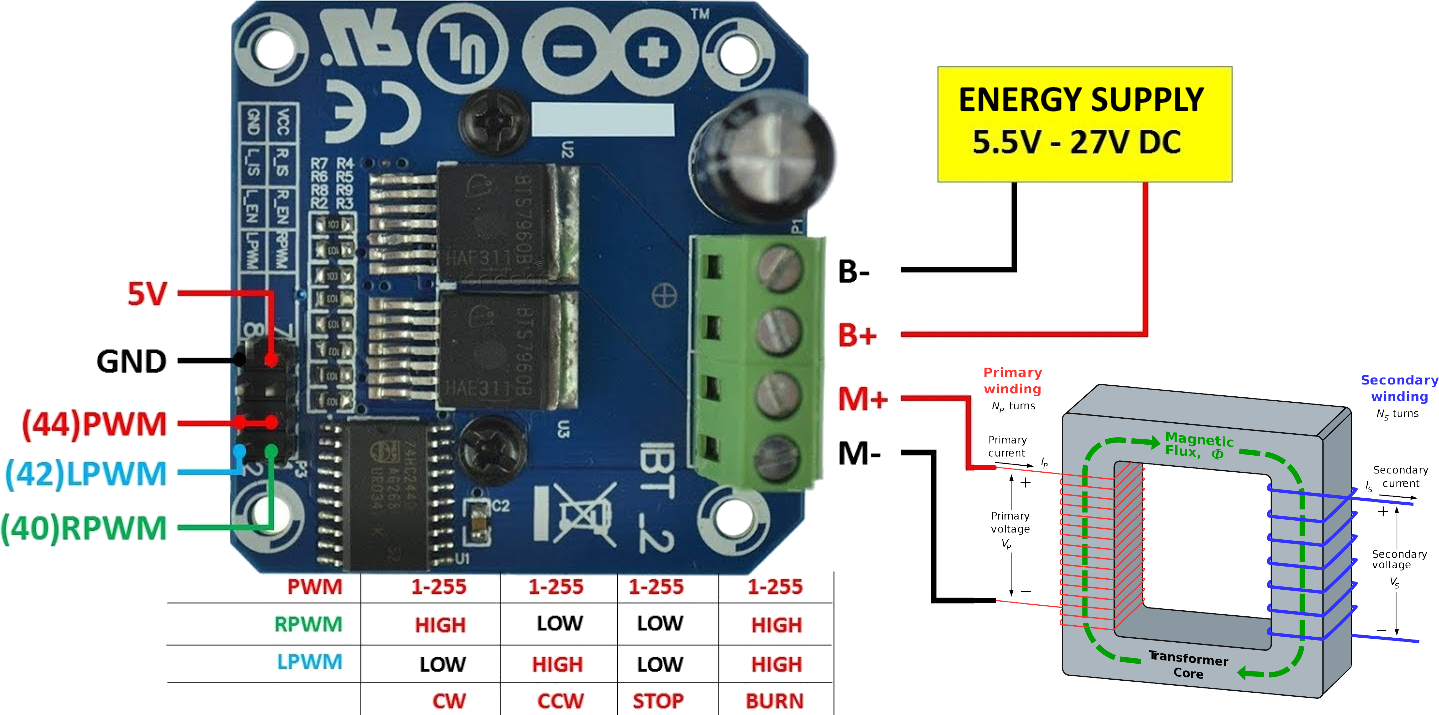
\includegraphics[width=1\textwidth]{IBT-2/TopView.png}
\end{figure}

\noindent
Esso non è un comune Ponte-H integrato: per poter gestire potenze superiori è stato costruito usando 2 Half-Bridge (\cite{BTS7960b}) collegati assieme mediante una opportuna logica per ricreare un normale Ponte-H.\\
Questa scheda in particola ha prestazioni interessanti per gli scopi di questa tesi, i principali sono elencati di seguito:\vspace{-8mm}
\begin{table}[H]
	\centering
	\caption[IBT-2 Specifiche]{IBT-2 Specifiche}
	\begin{tabular}[t]{|l r|}
		\hline
		Power Input Voltage:                                     & 6 -- 27 V \\
		Peak current:                                            & 43 A      \\
		Massima Frequenza di PWM:                                & 25 kHz    \\
		Protezione Sovra Tensioni                                &           \\
		Disaccoppiamento Ingresso di Potenza/Logica di controllo &           \\
		\hline
	\end{tabular}
\end{table}\vspace{-4mm}
\noindent
Di particolare interesse per l'esperimento è proprio la corrente di picco gestibile:
avendo le dinamiche del sistema tempi inferiori ai 5 secondi, poter reggere correnti di picco così elevate rende
la scheda perfetta per i nostri scopi.

\newpage
\subsection{Schema Elettrico}
Al suo interno il driver è composto da 2 Half-Bridge \cite{BTS7960b}, connesse secondo lo schema:
\begin{figure}[H]
	\centering
	\caption[IBT-2 Schema Elettrico]{IBT-2 Schema Elettrico}
	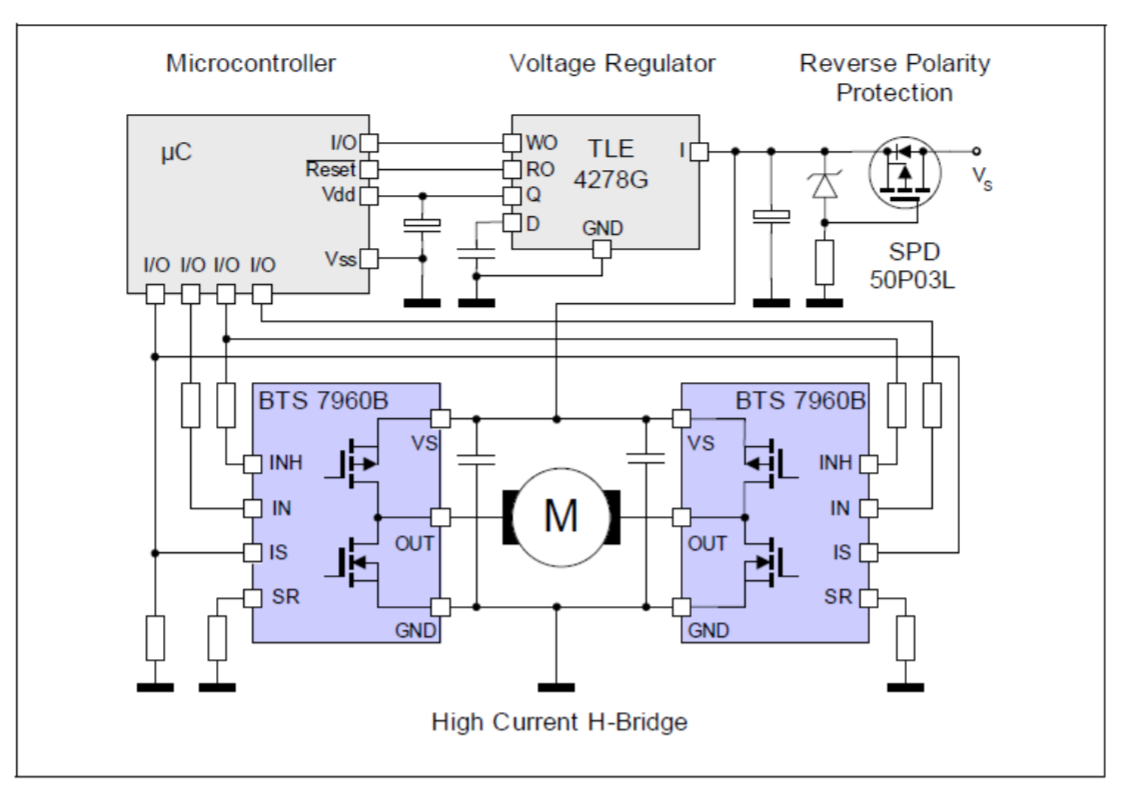
\includegraphics[height=0.5\textheight]{IBT-2/elettricScheme.png}
\end{figure}\vspace{-5mm}

\noindent
Il \microC è protetto dal carico connesso all'interno del \citefield{BTS7960b}{series}, lasciando al \microC solo il compito di controllare i segnali che commutano lo stato dei 2 Half-Bridge.
\newpage
\subsection{Connessione di Controllo}
Il driver permette 2 modalità di funzionamento:
\begin{description}
	\item[Doppio PWM] Modalità operativa che richiede l'uso di 2 PWM\\
	      Ciascun PWM controlla uno dei 2 Half-Bridge, e per evitare di bruciare i driver devono essere controllati singolarmente, il vantaggio di questa configurazione è la possibilità di usare 2 frequenze di controllo diverse.
	\item[Singolo PWM] Modalità operativa classica di un normale Ponte-H\\
	      In questa modalità, la porta nand presente sulla scheda attua la logica di controllo opportuna per governare i 2 Half-Brige come fossero un normale Ponte-H.
\end{description}

\noindent
Per il nostro esperimento si è scelto di usare il collegamento \textbf{\underline{Singolo PWM}} così da evitare spiacevoli sorprese e avere il PWM di controllo sempre sincronizzato.	

\newpage
\subsection{Benchmark del Driver}
Il driver sulla carta ha buone prestazioni, dal datasheet non risaltano \nonLinearita, esse invece sono presenti e per farle risaltare si sono effettuati 2 segnali di input:
\begin{enumerate}
	\item \nameref{lst:ondaTriangloare} \vspace{-3mm}
	      \begin{figure}[H]
		      \caption[Esperimento con Onda Triangolare]{Onda Triangolare}
		      \centering
		      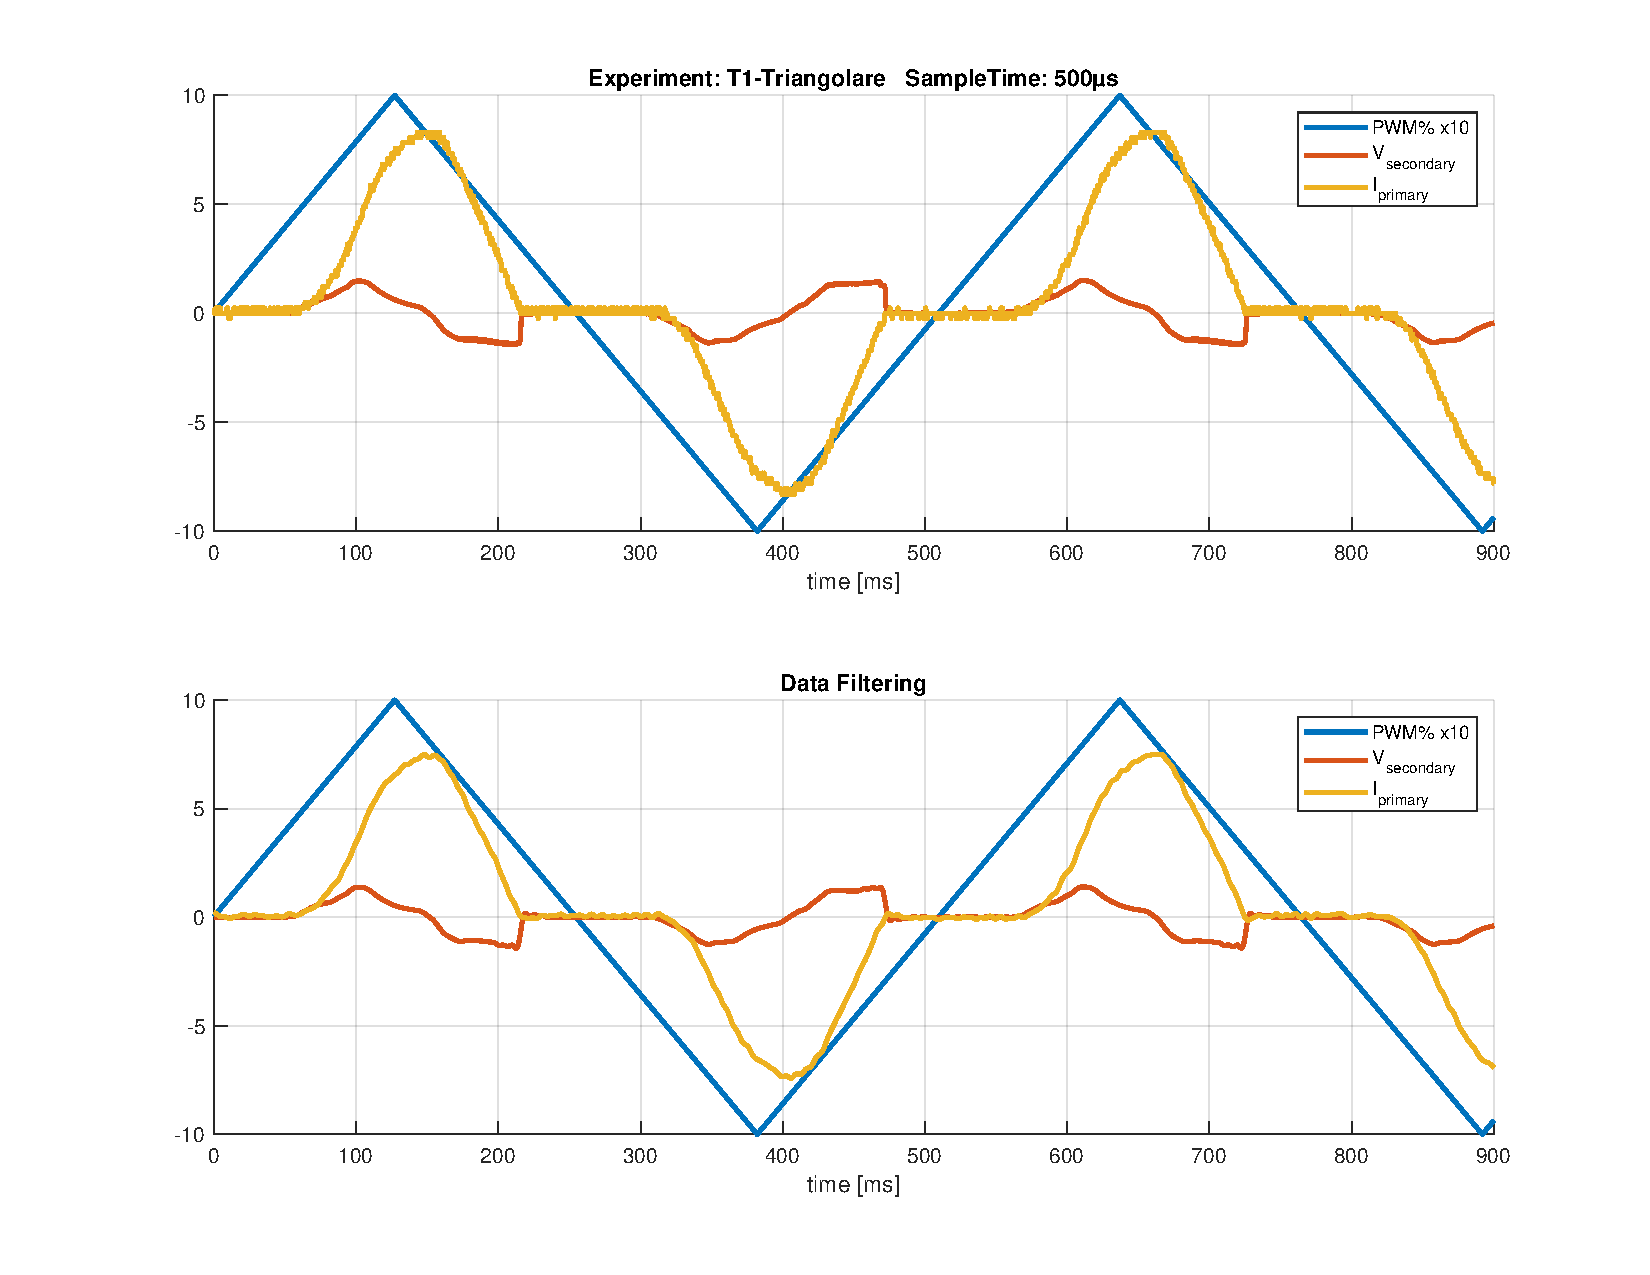
\includegraphics[height=0.5\textheight]{IBT-2/T1-Triangolare.pdf}
	      \end{figure}\vspace{-10mm}
	      \paragraph{Dead-Zone Inferiore} L'onda triangolare si presta bene per far risaltare la problematica della Dead-Zone Inferiore, infatti in tutti gli intorni in cui il segnale passa per 0, è possibile vedere come tanto la corrente quanto la tensione sul secondario non vari minimamente, indice evidente dell'assenza di corrente e quindi della presenza della \textbf{Dead-Zone}.\\
	      Per calcolare la soglia di \textbf{Dead-Zone Inferiore} è sufficiente vedere il primo valore di PWM  per cui il sistema risponde dopo il passaggio per 0.      
	      \newpage
	\item \nameref{lst:ondaTrapezoidale}  \vspace{-3mm}
	      \begin{figure}[H]
		      \centering
		      \caption[Esperimento con Onda Trapezoidale (\textit{Rapid Shot})]{Onda Trapezoidale (\textit{Rapid Shot})}
		      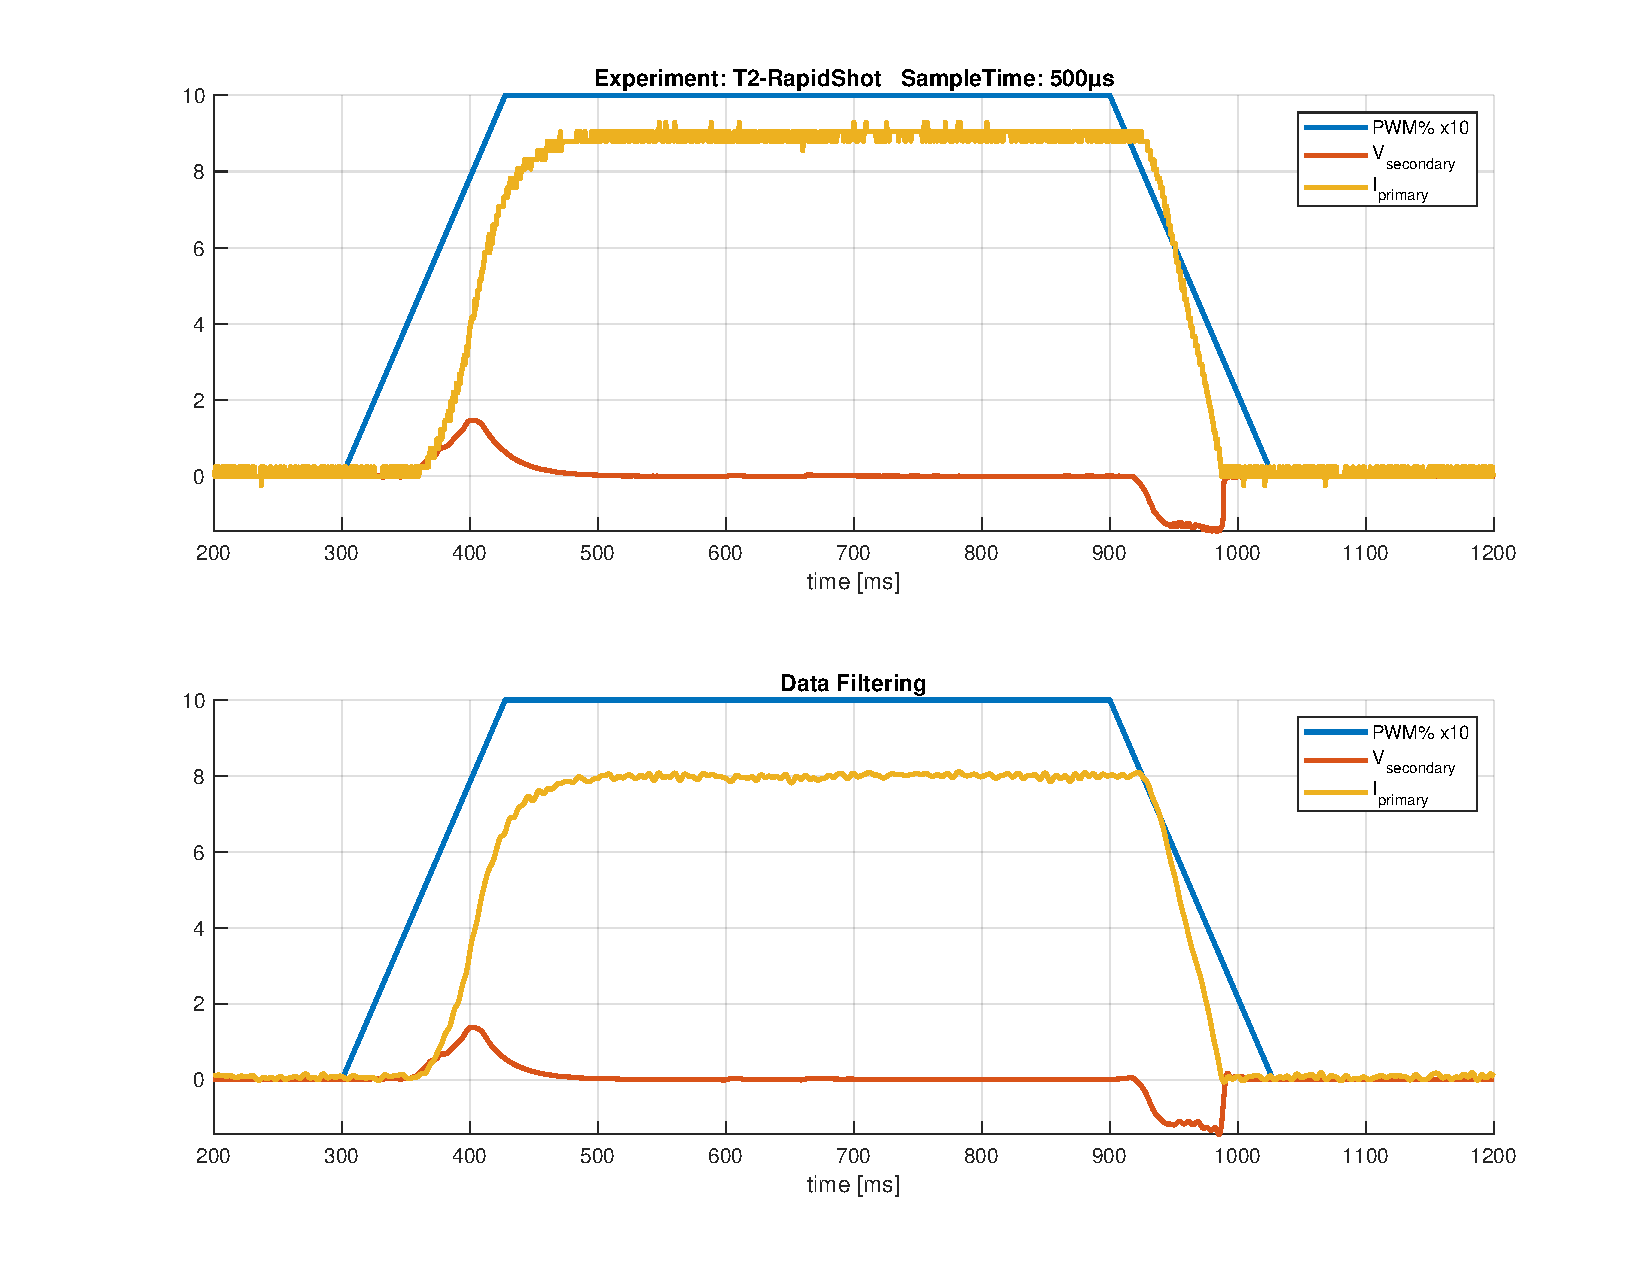
\includegraphics[height=0.5\textheight]{IBT-2/T2-RapidShot.pdf}
	      \end{figure}  \vspace{-15mm}
	      \paragraph{Dead-Zone Superiore} Usando il segnale \textit{Rapid Shot} mettiamo in evidenza la presenza della \textit{Dead-Zone Superiore}, visibile sotto forma di ritardo di attuazione nella rampa di discesa.\\
	      Il ritardo è pari a circa 20ms {\small \textit{(guarda 900ms)}}, e come detto è causato dalla seconda Dead-Zone presente nel driver.
\end{enumerate}
\noindent
Il driver soffre di questi problemi poichè per i Duty-Cycle \textit{Alti} e \textit{Bassi} nel PWM, prima uno e poi l'altro Half-Bridge, non fa in tempo a commutare che il segnale ha nuovamente cambiato valore, causando di fatto questa assenza di attuazione e quindi la Dead-Zone. Sapendo della presenza di queste 2 Dead-Zone, risaliamo ai loro valori di soglia andando a vedere l'inizio della risposta del secondario per entrambi i fronti:\vspace{-4mm}
\begin{table}[H]
	\centering
	\caption[Fasce della Dead-Zone]{Fasce della Dead-Zone}
	\begin{tabular}[t]{||c r||}
		\hline
		Dead-Zone Superiore & $\pm$ 210 PWM  \\
		Dead-Zone Inferiore & $\pm$ 120  PWM \\
		\hline
	\end{tabular}
\end{table}
\chapter{Architettura di Sistema}\label{cap:Architettura}

%\begin{minipage}{12cm}\textit{Se lo si desidera, utilizzare questo spazio per inserire un breve riassunto di ci\`o che verr\`a detto in questo capitolo. Inserire solo i punti salienti.}
%\end{minipage}

%\vspace*{1cm}

\section{Architettura ad alto livello}\label{sec:architettura}
Il progetto finale ha come obiettivo la realizzazione di un architettura di controllo per le bobine poloidali presenti nei reattori tokamak.

\begin{figure}[h] \label{fig:archietturaControllo}
	\centering
	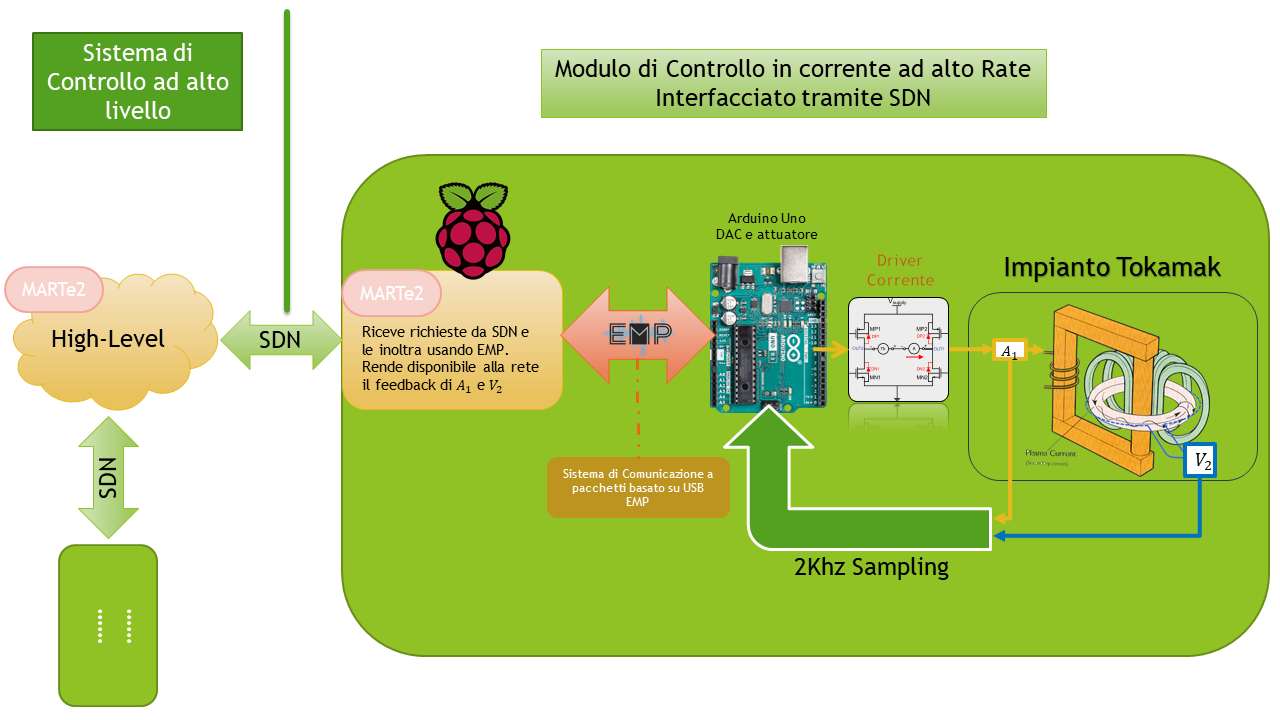
\includegraphics[width=1\textwidth]{Architettura/SystemArchitetture.png}
	\caption[Schema finale dell'archiettettura di controllo]{Architettura di controllo}
\end{figure}

\noindent
Lo schema proposto realizza l'obiettivo è controllare una singola bobina, il progetto finale prevederà la ripetizione in serie del medesimo schema per il numero di bobine necessarie.\\

Dallo schema risulta evidente che tutti i componenti visti nel capitolo "\nameref{cap:1}" si relazionano con lo stesso \microControllore: l'\ArduinoUno.\\
Per riportare i dati fuori e ricevere il riferimento da inseguire nella $V_2$, è stata realizzato il \nameref{EMP}, essa è stata scritta in C++ affinché possa essere Cross-Platform.\\
Il suo compito specifico, in questo progetto, è di mettere in comunicazione l'\ArduinoUno con un nodo \MARTe installato su di una \Rasp.\\
Quest'ultimo nodo ha il compito di mettere in rete il feedback dell'esperimento, e comunicare all'\ArduinoUno eventuali cambio di riferimento. Questo ultimo tratto è realizzato mediante il protocollo \textbf{SDN}, che viaggia sopra Ethernet e dà garanzie Real-time.\\
Nella sua forma finale, il progetto prevede la riproduzione in serie di questo schema di controllo per arrivare a controllare tutte le bobine poloidali presenti in un tokamak.

\newpage

\section*{EMP - Libreria di Comunicazione Seriale\\Embedded Message Pack }\label{sec:EMP}
\addcontentsline{toc}{section}{\protect\numberline{\thesection} EMP - Libreria di Comunicazione Seriale}

\begin{figure}[h]
	\centering
	
\includegraphics[width=1\textwidth]{EMP/EMP-Logo-Background.png}
\end{figure}
\paragraph{\citefield{EMP}{title}} nasce con l’obiettivo di standardizzare un protocollo e creare una libreria C++ basata su classi Template, che permetta di automatizzare e standardizzare tutto il lavoro di programmazione necessario all’invio/ricezione di dei pacchetti dal formato Pre-Concordati tra 2 Device connessi Peer2Peer (Nessuna pretesa di network-ing). (\cite{EMP})\\
Il raggiungimento dei suoi obiettivi, si sposa con la possibilità di supportare altre features interessanti:

\paragraph{Multiple-Package} Il protocollo di comunicazione che si è deciso di usare per EMP ha permesso di estendere il suo funzionamento e permettere il trasporto, attraverso lo stesso mezzo, di \textit{\textbf{pacchetti di tipologia e dimensione diversa}} all’interno della stessa libreria, evitando al contempo di inviare per ogni pacchetto più byte di quelli strettamente necessario. $\Rightarrow$ \textbf{Alta Efficienza}

\paragraph{Zero Tempo di negoziazione} Sempre grazie al protocollo di comunicazione, EMP è adatto ad un uso ‘Streaming’, questo perché non è necessario alcuna fase di sincronizzazione iniziale o durante la trasmissione in caso di perdita di dati, in aggiunta a ciò, EMP è in grado di scartare pacchetti errati in maniera trasparente all’utilizzatore. Tutto questo grazie al protocollo che \textbf{Auto-delimita i singoli pacchetti}. $\Rightarrow$ \textbf{Trasparenza Totale}

\paragraph{Responsabilità} Le uniche responsabilità a carico degli utilizzatori sono il riempimento dei pacchetti e la definizione degli stessi tra i 2 estremi della comunicazione.

\subsection*{Consistent Overhead Byte Stuffing (COBS)}
\addcontentsline{toc}{section}{\protect\numberline{\thesection} Protocollo - COBS}
Il protocollo di comunicazione che permette l’invio di \textbf{pacchetti diversi} e \textbf{senza fasi di negoziazione} alla base della libreria è \textbf{COBS}(\cite{COBS}).\\
Si tratta di un algoritmo per la codifica di byte, progettato per essere al tempo stesso efficiente e non ambiguo, che permette la definizione di \textit{data-pack frame} \textbf{Auto-delimiti} .

\begin{figure}[h]
	\centering
	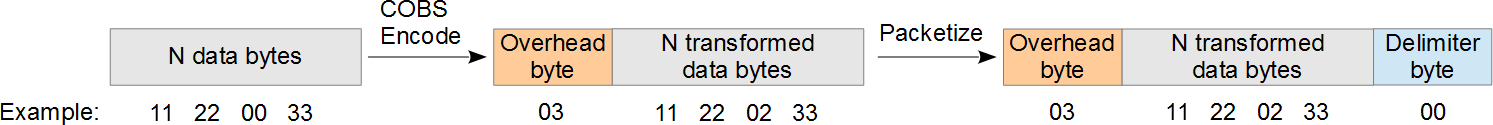
\includegraphics[width=1\textwidth]{EMP/Cobs_encoding_with_example.png}
	\caption[Esempio di COBS]{Esempio di COBS}
\end{figure}

\subsection{Metodo di codifica}
L'algoritmo di COBS trasforma una stringa arbitraria di byte, ciascuno dei quali ha un Range di valori da \textbf{[0:255]} in una nuova stringa di byte dove però ogni byte va da \textbf{[{\color{red}1}:255]}. La dimensione della nuova stringa è sempre pari alla dimensione della precedente + 1.\\
L'obiettivo di questo metodo di codifica è di eliminare tutti i possibili byte \zeroByte dal pacchetto in maniera reversibile.\\
Questo processo rende il carattere \textbf{\zeroByte (byte zero)} ottimo candidato per essere usato come terminatore di stringa durante l'invio, rendendo un pacchetto COBS-Encoded mai ambiguo e sempre \textbf{Auto-delimitato}.\\
L'algoritmo di codifica consiste nel:
\begin{enumerate} [itemsep=-3mm]
	\item Inserire un byte \zeroByte all'inizio del pacchetto
	\item Individuare tutti gli altri byte \zeroByte
	\item Inserire un byte \zeroByte alla fine del pacchetto
	\item Sostituire tutti gli \zeroByte con la distanza dal successivo \zeroByte nella stringa, ignorando l'ultimo
\end{enumerate}

\begin{figure}[h]
	\centering
	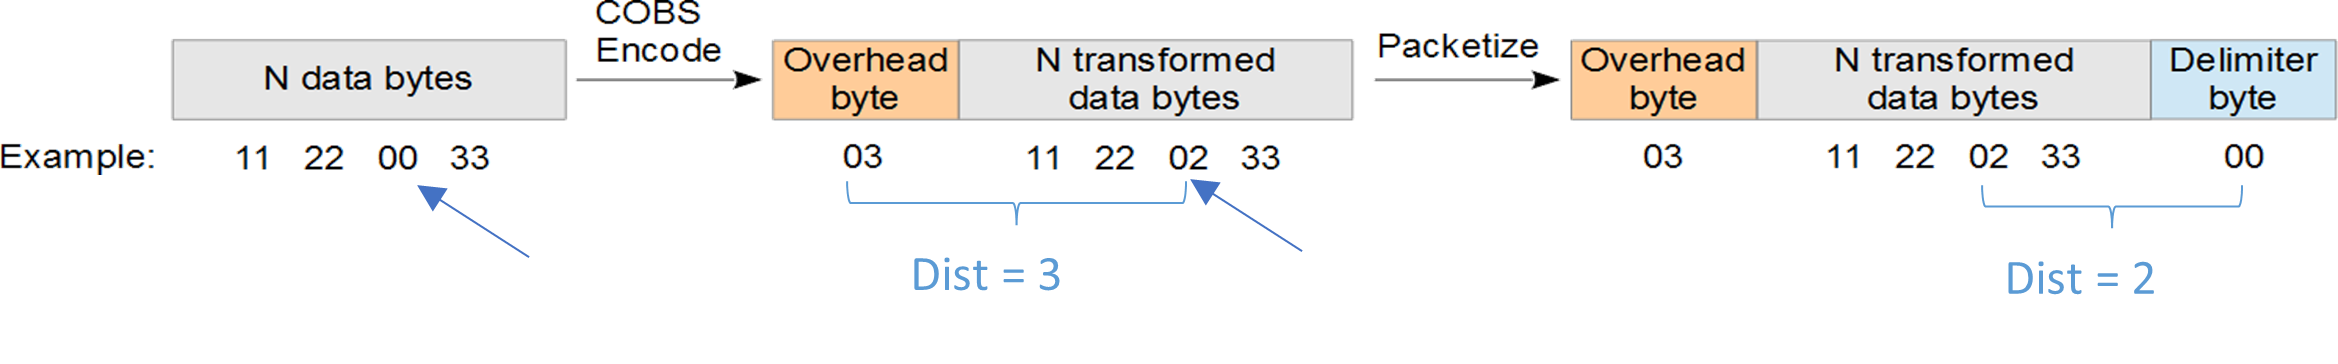
\includegraphics[width=1\textwidth]{EMP/Cobs_encoding_with_example-dist.png}
	\caption[Esempio di COBS con distanza]{Esempio di COBS con distanza}
\end{figure}

La versione usata per questo progetto, che comunque non ha l'obiettivo di trasmettere quantità infinite di byte, ha il limite di non poter codificare blocchi di byte che hanno una distanza tra 2 \zeroByte superiore a 255, questo limite è potenzialmente rimovibile usando un algoritmo più sofisticato.

\subsection{Caratteristiche chiave}
Prima caratteristica vincente della libreria è il suo alto grado di adattabilità, essa infatti per poter funzionare richiede solo \textbf{2 informazioni critiche} (e altre di contorno per l'allocazione opportuna dei buffer), esse sono i tipi dei pacchetti in \textbf{ Input} (\textit{pIn}) e in \textbf{Output} (\textit{pOut}) ovvero sia delle strutture in C, con i dati organizzati in base al messaggio da trasferire (\nameref{lst:EMPpackDef}).\\
In secondo luogo, la codifica \citefield{COBS}{title}, che abbiamo appena visto permette di avere pacchetti \textbf{Auto-delimitati}, ciò permette quindi di scambiare pacchetti diversi tra loro (sia per tipologia che per lunghezza) lungo \textbf{lo stesso} \textit{Stream} di dati.\\
L'unica condizione neccessaria è che il destinatario sia capace di determinare la tipologia di contenuto trasportato nel pacchetto semplicemente leggendolo.\\
Questo può essere facilmente risolto in più modi:
\begin{spacing}{1.5}
	\begin{description}
		\item[Lunghezza Univoca] Ogni possibile pacchetto ha una lunghezza diversa da tutti gli altri, $\Rightarrow$ la lunghezza implica il contenuto
		\item[Aggiunta di un campo Tipologia] Aggiungendo al’inizio della trasmissione un \textit{type byte}, ovviamente Pre-Concordato, diventa possibile per chiunque sapere come interpretare il contenuto del pacchetto.
	\end{description}
\end{spacing}
\noindent
Il metodo più universale è sicuramente l'aggiunta di un campo fisso per il tipo, di cui un esempio è visibile nell'appendice al listato \ref{lst:EMPmultiplePack}. (\nameref{lst:EMPmultiplePack})

In ogni caso, la codifica \citefield{COBS}{title} aggiunge 2 byte extra al pacchetto che si vuole inviare, e tanto per la codifica quanto per la decodifica in ricezione, il \textbf{costo} è sempre pari a \textbf{O(n)}.

\begin{multicols}{2}
	\begin{center}
		{\large Vantaggi:}
	\end{center}
	\begin{spacing}{1.25}
		\begin{enumerate}[itemsep=-1mm]
			\item Pacchetti {\color{Azure}\textbf{Self-Delimited}}
			\item Canale {\color{Azure}\textbf{Multi-Packet ready}}
			\item Protocollo {\color{Azure}\textbf{Senza Negoziazioni}}
			\item All’utilizzatore è richiesto solo di Pre-Concordare il formato del pacchetto con l’altro lato dello stream
			\item Prerequisiti implementativi minimale (mezzo di comunicazione a bytes di tipo \textit{peer2peer} asincrono)
		\end{enumerate}
	\end{spacing}
	\vfill
	\columnbreak
	\begin{center}
		{\large Svantaggi:}
	\end{center}
	\begin{spacing}{1.25}
		\begin{enumerate}[itemsep=-1mm]
			\item Aggiunge 2 byte fissi
			\item Richiede O(n) elaborazione sia in codifica che decodifica
		\end{enumerate}
	\end{spacing}
	\vspace*{\fill}
\end{multicols}

\newpage

\subsection{Integrità dei pacchetti}
Per aumentare ulteriormente i campi d’uso e garantire un layer minimale di \textbf{integrità} sui pacchetti in transito, la libreria è stata progettata per include in maniera trasparente anche un un check di errore calcolato usando \cite{CRC8}, aggiunto in trasmissione e rimosso in ricezione.\\
L'aggiunta e il calcolo del CRC8 viene fatta sul pacchetto non ancora \textit{COBS-Encodato}, ciò garantisce la possibilità di inviare il pacchetto a prescindere da quale sia il risultato del CRC8, e viene quindi verificato dopo aver de-\textit{COBS-Encodato} il pacchetto in ricezione.\\
Questa features deve essere attiva o disattivata da entrambi i lati della libreria (ne consegue che anche lei deve essere pre-concordata tra i 2 estremi).\\
La libreria, se attiva, è in grado di capire se il pacchetto ha subito degli errori (ovviamente nei limiti del CRC8) e in tal caso scarta il pacchetto ricevuto in maniera totalmente trasparente all'utilizzatore.\\
L’aver usato COBS come sistema di codifica per la trasmissione, garantisce che la decodifica debba avvenire solo nei byte compresi tra 2 zeri, e se questa decodifica presenta un errore, toglie ogni ambiguità sul da farsi poiché il pacchetto viene scartato e si attende un successivo 0 mentre si memorizzano i byte ricevuti nel frattempo.

\newpage
\subsection{Struttura del codice}
Lo sviluppo del codice è qui riassunto nel \textbf{Class Diagram} fatto in UML, del codice:\\
\begin{figure}[h]
	\centering
	\includegraphics[width=1\textwidth]{EMP/EMP-Hierarchy.png}
	\caption[Class Diagram UML di EMP]{Class Diagram UML}
\end{figure}

\noindent
Senza entrare eccessivamente nel dettaglio di \citefield{EMP}{title}, essendo tutto reperibile nella versione più aggiornata all'interno del repository di \cite*{EMP}, osserviamo che il codice è diviso in 2 macro blocchi (\textbf{MPCore}, \textbf{MP}) più una classe di supporto per il buffer circolare.\\
Questa organizzazione del codice è stata pensata per far compilare su tutte le piattaforme di interesse lo stesso \textit{codice attivo}(codifica e decodifica dei pacchetti + accumulo), e demandare le particolarizzazioni dovute alle varie piattaforme o al mezzo di comunicazione usato nel caso specifico a delle classi figlie.\\
\begin{spacing}{1.25}
	\begin{description}
		\item[MPCore] Il \textit{Codice attivo} è presente all'interno del package \textbf{MPCore}. Tutto il codice contenuto in questo package è scritto in C++11 e per essere compilato necessita di un set minimale di librerie standard, sicuramente presenti in ogni piattaforma di sviluppo.
		\item[EMP] Il package più generico comprende le classi figlie che concretizzano le operazioni di invio e ricezione, facendo poi elaborare i byte al codice che ereditano dalla classe \textbf{MP}.\\
		      Le classi sono scritte e pensate per funzionare su una piattaforma specifica, e su essa essere ottimizzate.\\
		      Se la piattaforma lo concede come nel caso di Linux, è quindi possibili fattorizzare ulteriormente delle funzionalità comuni e scrivere così, via via, sempre meno codice sicuri che quello in comune, se funziona su una classe, deve funzionare anche per l'altra.
		\item[Buffer Circolare] La classe \textit{CircularBuffer} è una classe di supporto che implementa un buffer circolare con logica "\textit{One Slot Open}"(\cite{CircularBuffer}) attraverso una classe template.\\
		      Il motivo di questa scelta, molto forte e vincolante, essendo principalmente lei la causa per cui tutte le altre sono anch'esse template, è dovuta alla possibilità di istanziare in fase di compilazione, tutta la memoria richiesta per il funzionamento del programma.\\
		      Una simile necessità nasce dal dover compilare la classe anche su schede embedded, le quali, notoriamente, non hanno a disposizione un heap in ram spazioso per la memoria dinamica, e beneficiano nelle prestazioni se in fase di compilazione gli indirizzi di memoria sono fissi.
	\end{description}
\end{spacing}

\subsection{Logica di Comunicazione}
La libreria è pensata per automatizzare la trasmissione e la ricezione di 2 tipologie di pacchetti \textit{Pre-concordati} tra 2 realizzazioni di \textbf{MP}, ovviamente non necessariamente sullo stesso dispositivo.\\
Come riportato in appendice (\ref{EMPCode}), la definizione dei pacchetti è molto comoda, e usando un tipo e le \verb|union| è anche possibile gestire la comunicazione di pacchetti diversi tra i 2 lati della comunicazione, basterà invertire l'ordine dei pacchetti tra le 2 classi.\\
Il riempimento corretto dei dati nel pacchetto, il calcolo della size utile e il riconoscimento in ricezione del pacchetto trasmesso, è tutto a carico dell'utilizzatore della libreria, essa garantisce la corretta ricetrasmissione e di svegliare un ascoltatore al ricevimento di un pacchetto, qualunque sia la sua lunghezza.


\newpage
\subsection{Code Flow}\label{sub:codeFlow}
Vediamo ora come la libreria si frappone tra 2 device che vogliono comunicare mediante questo sequence diagram:\\
\begin{figure}[h]
	\centering
	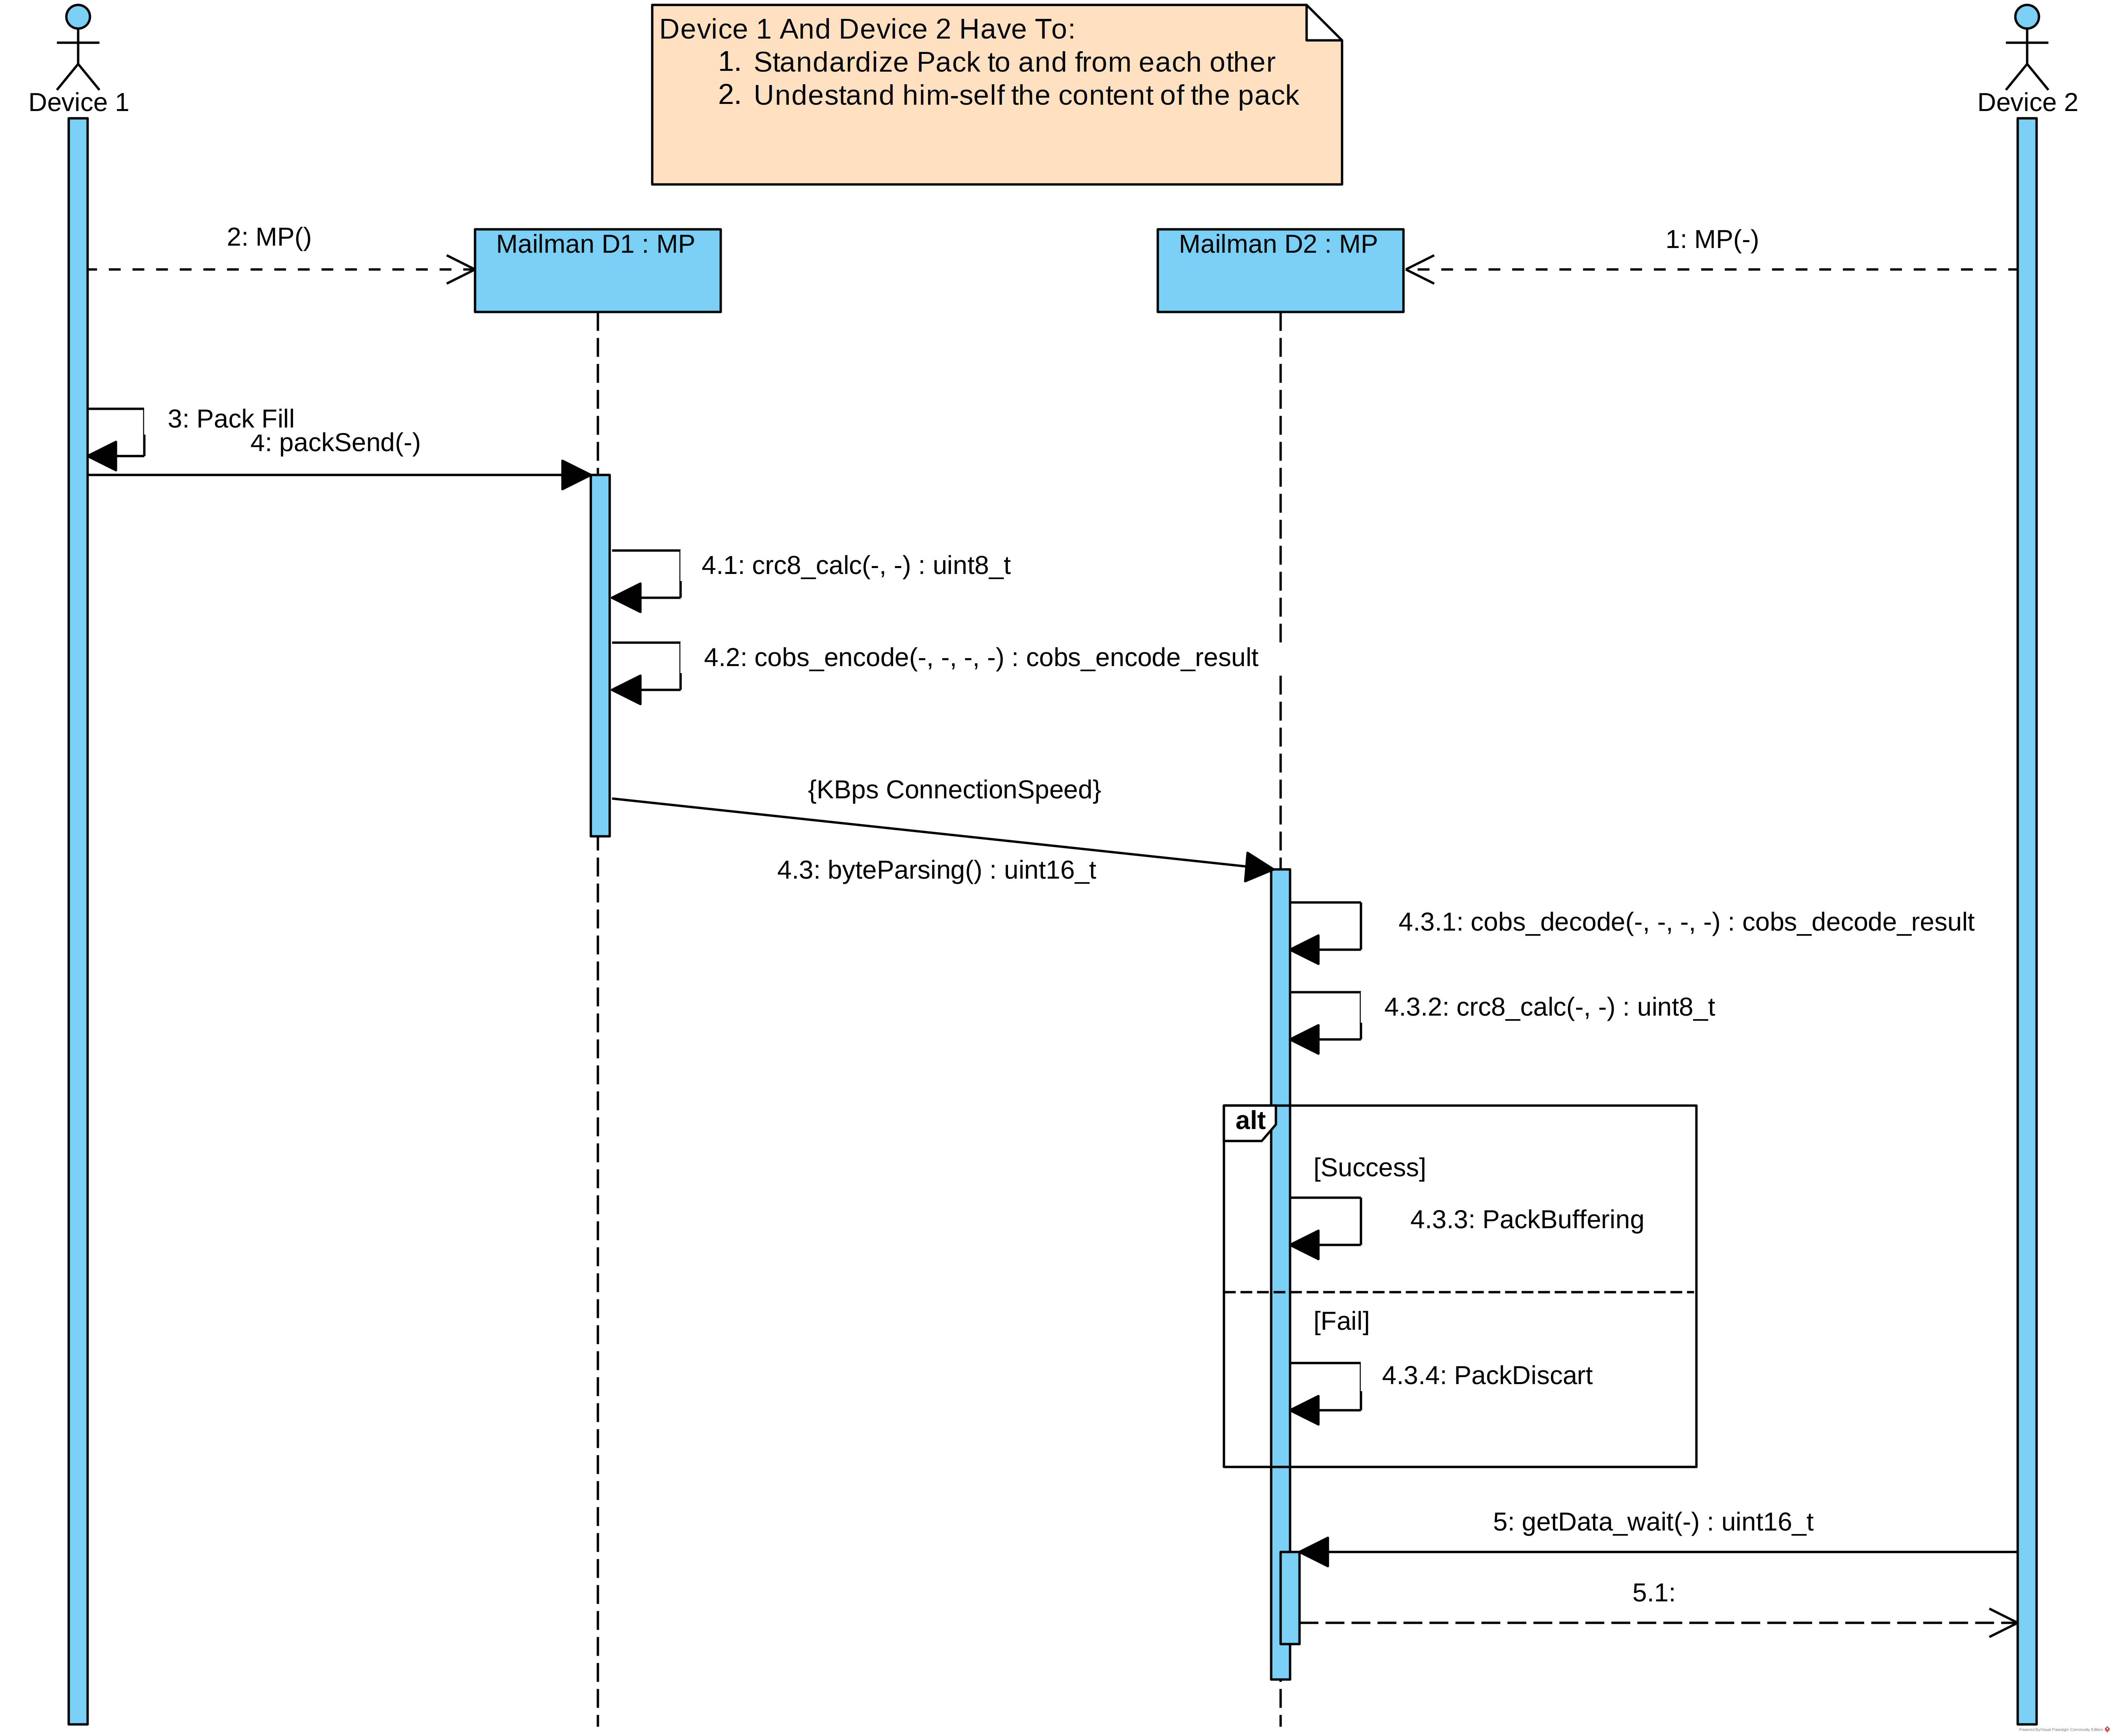
\includegraphics[width=1\textwidth]{EMP/Message Pack Sending Flow.png}
	\caption[Sequence Diagram UML di EMP]{Sequence Diagram UML}
\end{figure}

\noindent
In questo esempio generico i 2 device non sono definiti, ovviamente nessuno dei 2 può istanziare concretamente una classe \textbf{MP}(essendo una classe virtuale), ma come detto prima, tutti i \textit{Codici attivi} sono racchiusi lì dentro.\\
Come si può osservare, eccetto il riempire i dati, inviarli e attendere che arrivi qualcosa, per gli attori il lavoro finisce subito, internamente alla libreria, invece, a parti invertite, abbiamo il calcolo del CRC8 (\cite{CRC8}) e la codifica usando COBS (\cite{COBS}), e l'omologo dall'altro lato, dopo aver ricevuto i byte, procede alla de-codifica e check per l'integrità.\\

\subsection{Test di Codifica/Decodifica su ogni Device}
La serie di passi descritta nel \nameref{sub:codeFlow} è stato testato su i vari dispositivi per cui la libreria è stata sviluppata usando il seguente schema:
\begin{figure}[h]
	\centering
	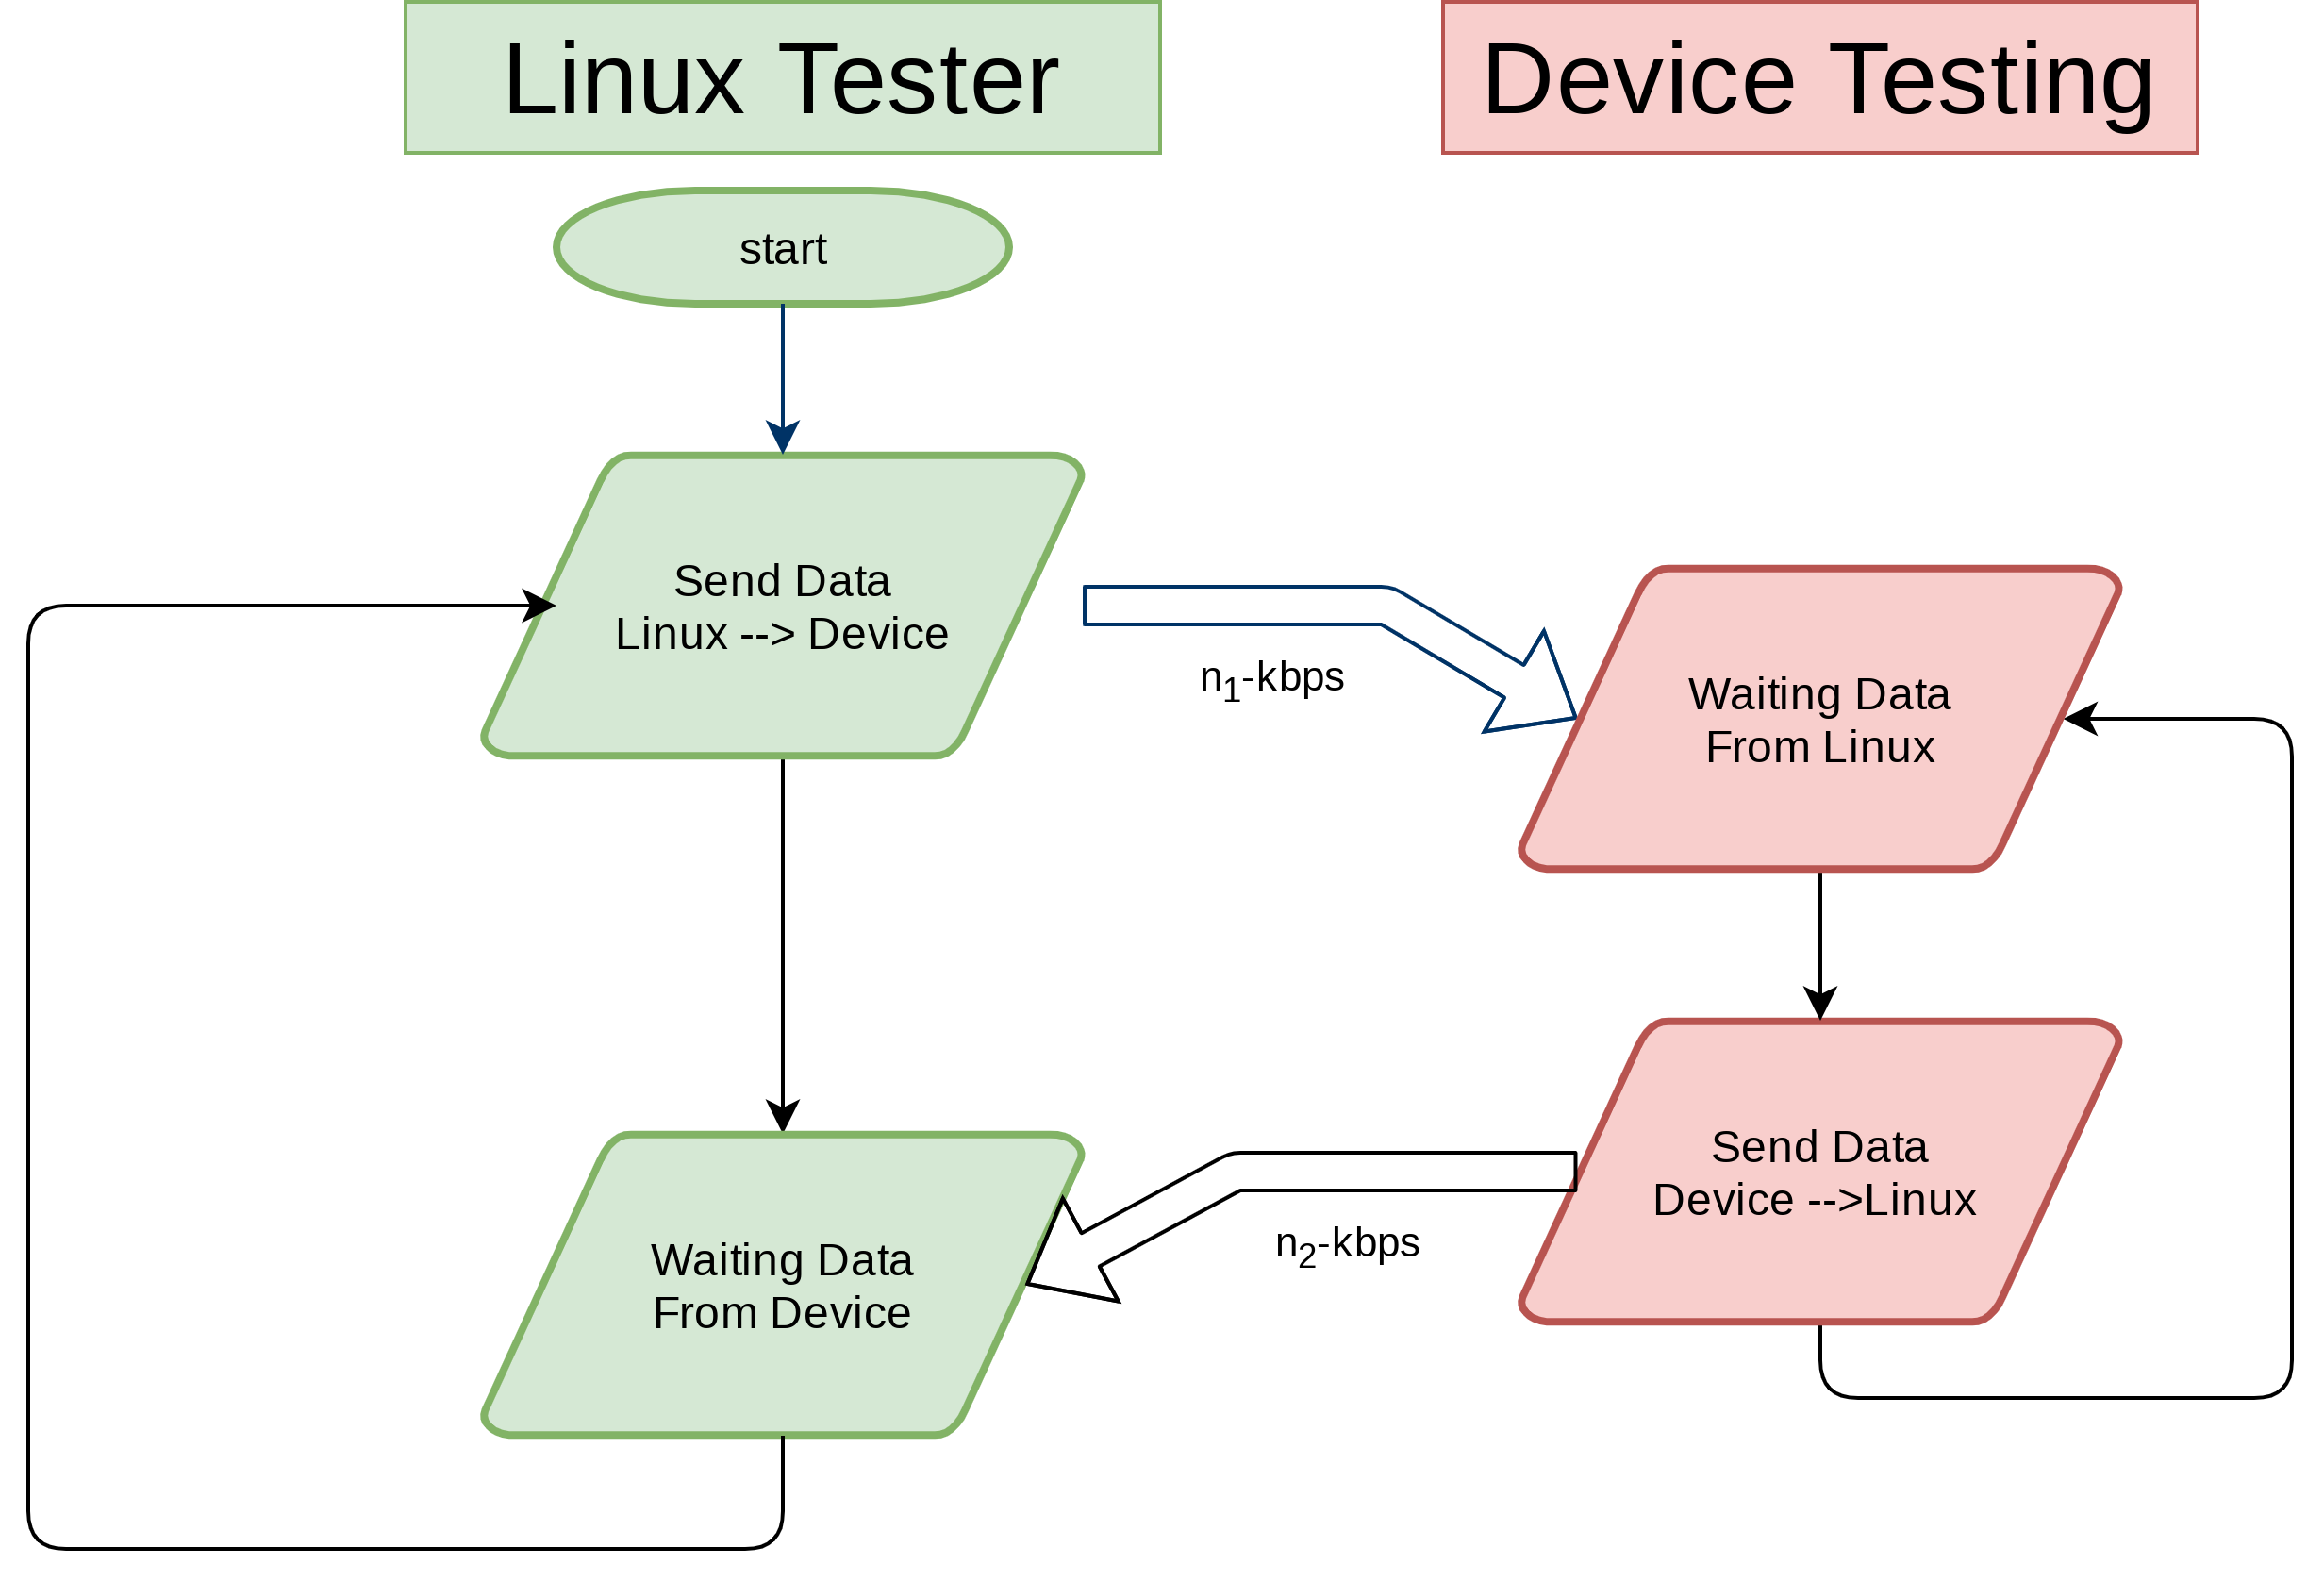
\includegraphics[width=0.8\textwidth]{EMP/TestFlow.png}
	\caption[EMP Benchmark Testing Flow]{Testing Flow}
\end{figure}

\noindent
I test vengono avviati da \textbf{Linux} e puntano a testare la perdita la correttezza della trasmissione usando \citefield{EMP}{title}, e il funzionamento di Encoding e Decoding delle classi sulle entrambe le architetture.\\
Ad ora, sulle 3 Piattaforme di sviluppo (Linux, Arduino, STM32) i test sono stati un pieno successo.

\newpage
\section{Online Sampling}
Come descritto in figura \ref{fig:archietturaControllo}, il sistema controlla internamente la corrente, ma comunica con il mondo fuori l'attuale stato della bobina.\\
Per comunicare i Sample (e ricevere le Reference) è stata infatti sviluppata \citefield{EMP}{title}(Sezione \ref{sec:EMP}).\\
Come visto nella sezione "\nameref{sub:parametriMisurati}", il circuito di misura è quello riportato in figura \ref{fig:circuitoDiMisura}.\\
E, come per il \nameref{CurrentSense}, in realtà anche il voltmetro $V_2$ possiede un offset a $\frac{V_{cc}}{2}$, aggiunto per poter misurare tanto le correnti positive, quanto quelle negative.
\begin{figure}[h]
	\centering
	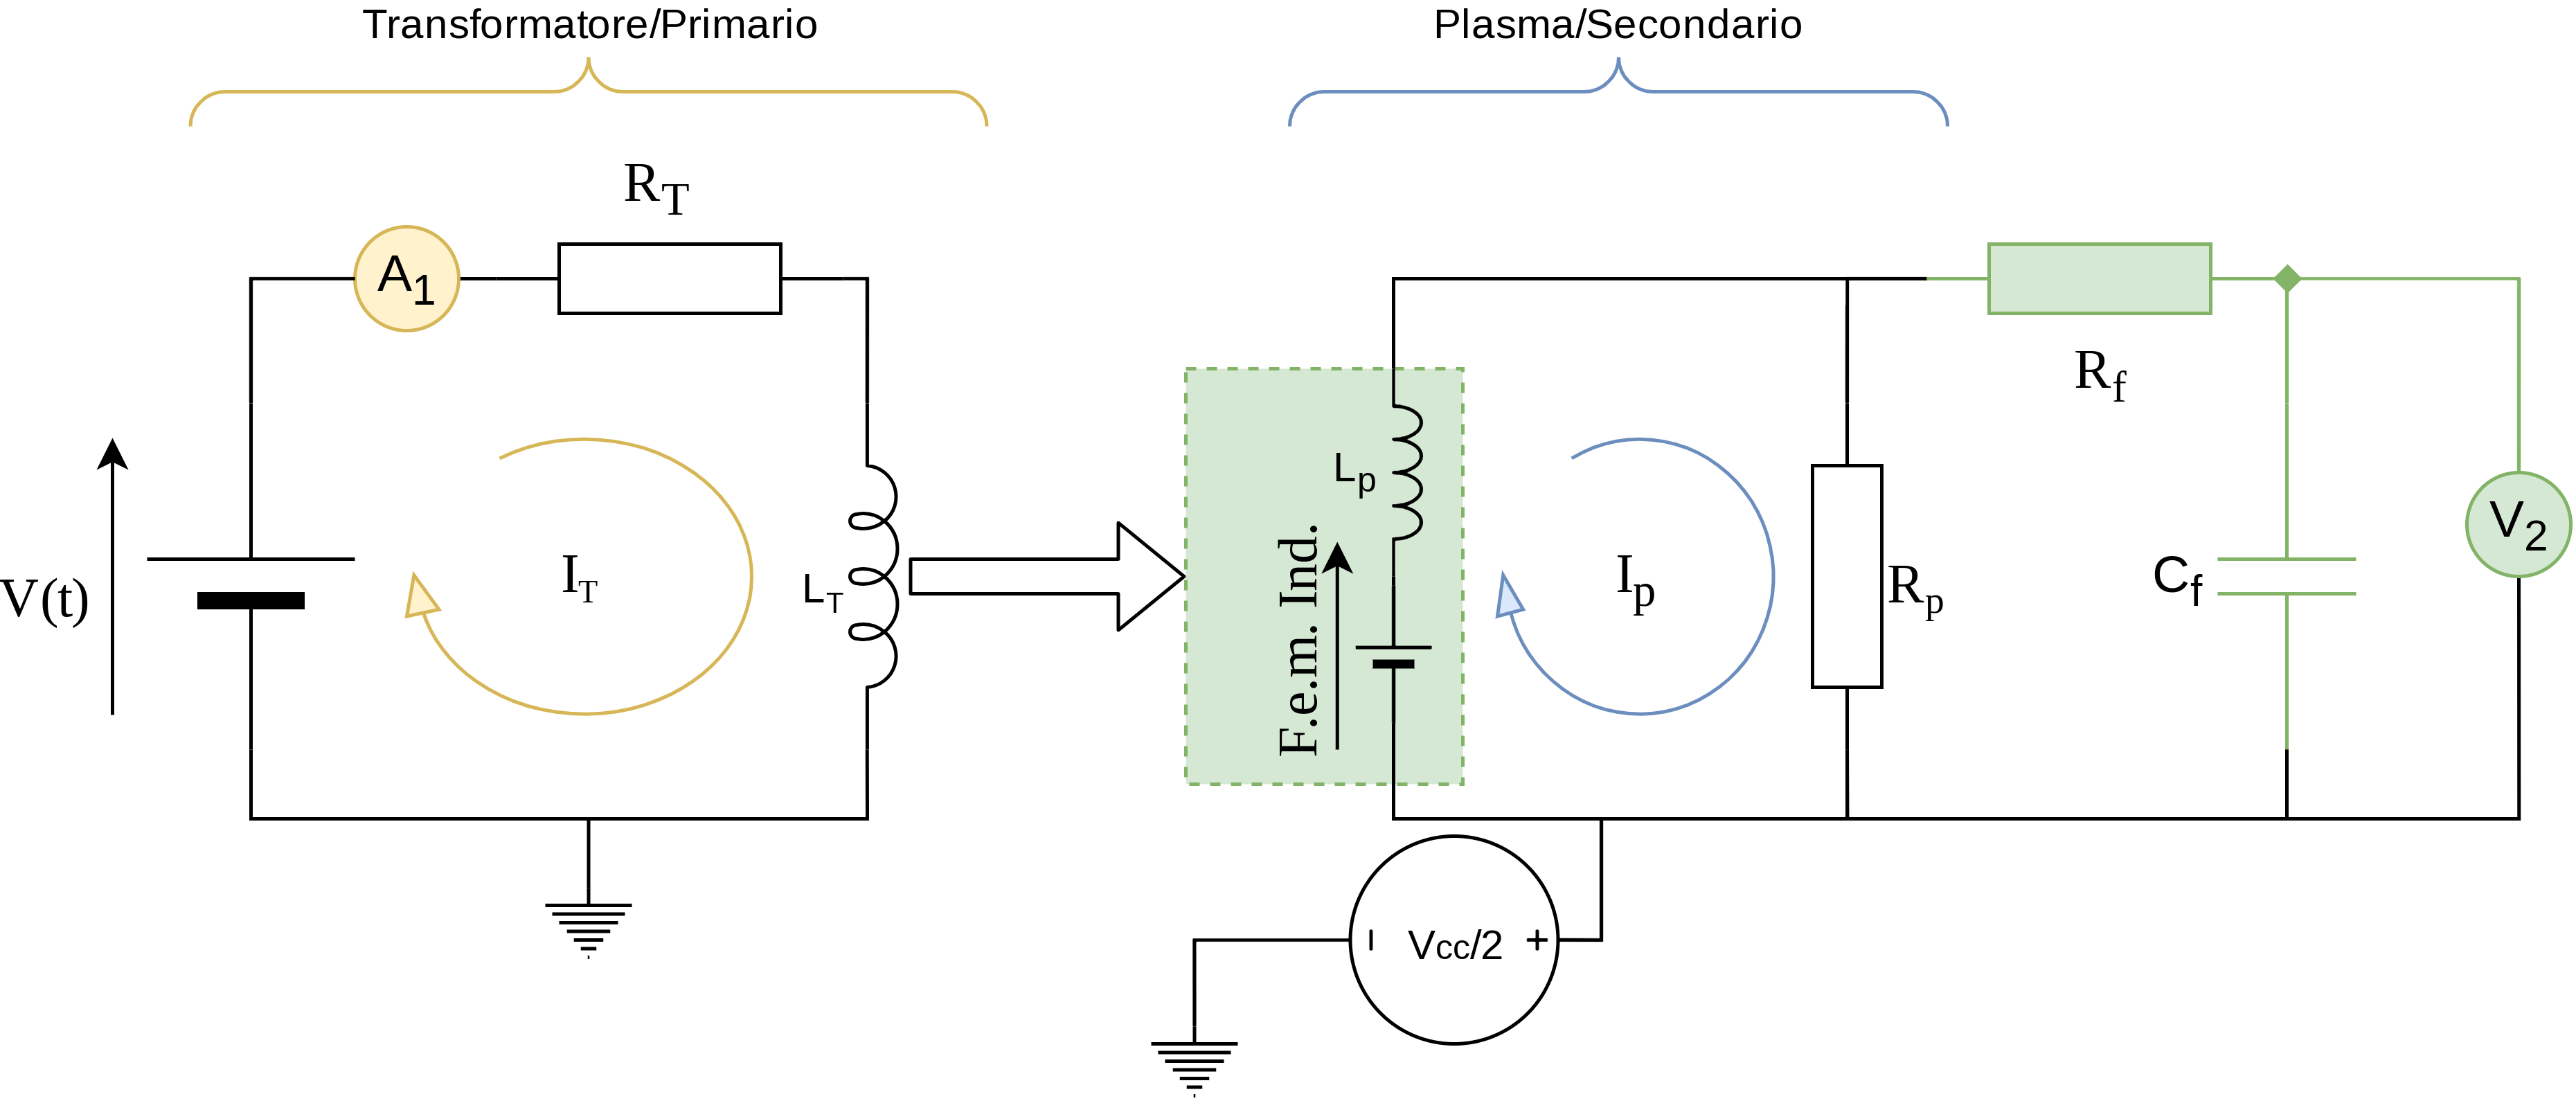
\includegraphics[width=1\textwidth]{Trasformatore/PlasmaCircuit-MisureCircuitOffset.png}
	\caption[Circuito equivalente del Plasma con l'offset delle Misure]{Circuito reale con Misure}
\end{figure}

\noindent
Controllo e misure avvengo alla massima frequenza che l'Arduino è riuscito effettivamente a gestire, ovvero 0.5ms (2Khz), nei quali campiona lo stato del sistema, genera il nuovo valore del PWM per il controllo di $V(t)$, e invia i dati attraverso \citefield{EMP}{title}.

\newpage
\subsection{Interconnessione \microControllore $\Leftrightarrow$ Companion}
Per raggiungere gli obiettivi descritti nella sezione dell'\nameref{sec:architettura}, i seguenti pacchetti multipli sono stati concordati tra le 2 parti:
\begin{lstlisting}[style=cppStyle,caption={Pacchetti Companion $\Rightarrow$ \microControllore   },label=lst:Companion2ArdPack]
// #######################################################
// ########        Companion to Arduino           ########
// #######################################################
struct newRef {
	int16_t newRef;
} __attribute__((packed));

struct setUpPackAsk {
	int8_t padding;
} __attribute__((packed));

enum LinuxSendType : uint8_t { newRefType, askType };

struct _packLinux2Ard {
	LinuxSendType type;
	union {
		struct newRef ref;
		struct setUpPackAsk ask;
	};
} __attribute__((packed));
typedef struct _packLinux2Ard packLinux2Ard;
\end{lstlisting}

\begin{lstlisting}[style=cppStyle,caption={Pacchetti \microControllore $\Rightarrow$ Companion },label=lst:Ard2CompanionPack] 
// #######################################################
// ########        Arduino to Companion           ########
// #######################################################
struct sample {
	int16_t pwm;
	int16_t V2_read;
	int16_t Isense_read;
	int16_t err;
} __attribute__((packed));

struct setUpPack {
	int16_t V2_mean;     // Adc read
	int16_t Isense_mean; // Adc read
	int16_t dt;          // Time in us (10^-6)
} __attribute__((packed));
enum ardSendType : uint8_t { sampleType, setUpPackType };

struct _packArd2Linux {
	ardSendType type;
	union {
		struct sample read;
		struct setUpPack setUp;
	};
} __attribute__((packed));
typedef struct _packArd2Linux packArd2Linux;
\end{lstlisting}
\noindent
Essi permettono al Companion di conoscere tutto quello che sta succedendo nel \microC, con un piccolo ritardo dovuto alla trasmissione ed eventuali ritardi interni (nel caso di Linux dovuti allo scheduler).
Le informazioni riguardanti offset e parametri dell'esperimento (\verb|struct setUpPack|), sono raccolti a macchina spenta, all'accensione della scheda nel \nameref{lst:controlSetup}.\\
Successivamente la scheda evolve per tic di 0.5ms, dove nel tempo morto resta in ascolto di eventuali pacchetti di richiesta da parte del Companion all'interno del \nameref{lst:controlLoop}.\\

\subsection{Storage su file delle informazioni}\label{subsec:experimentStorage}
Le informazioni ricevute dal Companion, vengono salvate all'interno di un file di testo contenente 2 tabelle, disposte una sotto l'altra.\\
La prima delle 2, tabula i dati del pacchetto \verb|struct setUpPack|, il quale risulta utile per poter interpretare i dati successivamente.
\begin{table}[h]
	\centering
	\begin{tabular}[t]{|c|c|c|}
		\hline
		$ V_{2_{mean}} $ & $ I_{sense_{mean}}$ & dt  \\
		\hline
		510              & 510                 & 500 \\
		\hline
	\end{tabular}
	\caption[Salvataggio di "struct setUpPack"]{Salvataggio di "struct setUpPack"}
\end{table}

\noindent
La seconda invece è lo streaming dei dati \verb|raw|, ottenuti dalla scheda:
\begin{table}[h]
	\centering
	\begin{tabular}[t]{|c|c|c|c|}
		\hline
		PWM   & $ V_{2_{read}}$ & $ I_{sense_{read}}$ & e     \\
		\hline
		0     & 509             & 510                 & 1     \\
		0     & 509             & 511                 & 1     \\
		\dots & \dots           & \dots               & \dots \\
		0     & 509             & 510                 & 59    \\
		44    & 510             & 510                 & 36    \\
		48    & 518             & 510                 & 28    \\
		53    & 514             & 510                 & 32    \\
		59    & 513             & 510                 & 33    \\
		\dots & \dots           & \dots               & \dots \\
		\hline
	\end{tabular}
	\caption[Salvataggio di "struct sample" $\forall$ dt]{Salvataggio di "struct sample" $\forall$ dt}
\end{table}
\noindent
Essi sono salvati sotto forma di testo ascii normale, separando i campi con un \verb|'tab'|.

\newpage
\section{Post Elaborazione con Matlab}
I dati salvati su hardisk, come visto della sezione \nameref{subsec:experimentStorage}, vengono presi in ingresso da Matlab.


\subsection{Conversioni Dati}
\subsection{Creazione dei grafici e Filtraggio}

\chapter{Stima del modello del sistema}\label{cap:stimaModello}

\begin{minipage}{12cm}\textit{
		In questo capitolo viene affrontato il problema della stima dei parametri del modello reale, in un equivalente lineare matematico, necessario per le simulazioni future e validare i risultati matematici precedenti.}
\end{minipage}

\vspace*{1cm}
\noindent
Partendo dall'esperimento con l'\nameref{lst:ondaTrapezoidale} per eccitare il sistema senza raggiungere la saturazione della tensione $ V_2 $ (ricordiamo che in uscita abbiamo un derivatore filtrato, quindi ogni onda quadra genera automaticamente una forte derivata), si è puntato a ricavare un modello lineare prima della corrente in $ I_T $ e successivamente della tensione $ V_2 $.\\
Essendo il driver di corrente intrinsecamente non lineare, specie nei pressi della Dead-zone, il cui taglio si è visto non essere netto come si spererebbe, si è cercato di ottenere un buon fitting nei transitori del sistema, dove la dinamica è più lineare e "pulita".\\
Questa stima è ovviamente semi-qualitativa (non troppo affidabile) e ha lo scopo di fornire un modello dell'impianto reale da usare in simulazione durante lo sviluppo del sistema di controllo, le \nonLinearita presenti vengono in questo modello ignorate, ma avendo dinamiche molto rapide, il controllo pensato per il modello lineare che stiamo per ricavare vedremo in seguito, continua ad essere valido anche nel caso reale \nonLineare.\\
Il modello stimato è per $ P_{pos} $ (eq \ref{eq:FuncTrasfTotPos}), al fine di renderne la trattazione più semplice evitando di confondersi con i segni.

\newpage

\section{Metodo di stima automatico}
Il metodo di stima automatico è basato sull'uso del \cite*{IdentificationToolbox} di Matlab, ed è usato allo scopo di ottenere una funzione di trasferimento SISO tra l'ingresso del Duty-Cycle (PWM) e la tensione sul secondario $ V_2 $.\\
Avendo a disposizione anche i dati della corrente sul primario, anche se poco sensibili, si è deciso di dividere la stima in 2 fasi per semplificare il lavoro al Toolbox: prima si è stimato il modello della \textbf{Corrente del Trasformatore} ($ I_1 $), e a causa della sua scarsa sensibilità di misura (risultato \ref{result:Istep}) si è usato il segnale ricostruito come ingresso per la stima della dinamica della tensione sul secondario.\\
Il numero di \textit{Poli} e \textit{Zeri} di entrambe le funzioni di trasferimento sono state scelte partendo dall'analisi teorica descritta nella sezione \nameref{subsec:ModelloFisico}, e il codice è presente in appendice a \nameref{lst:autoEst}.

\begin{table}[H]
	\centering
	\caption[Stime parametri con \cite*{IdentificationToolbox}]{Stime parametri con \cite*{IdentificationToolbox}}		\label{tab:stimaAutomaticaParametri}
	\vspace{1mm}
	\begin{tabular}[t]{||l|c|c||}
		\hline
		\multicolumn{1}{||c}{\textbf{Funzione}}            & \multicolumn{1}{|c}{\textbf{Input}} & \multicolumn{1}{|c||}{\textbf{Output}} \\
		\hline\hline
		                                                   &                                     &                                       \\[-3mm]
		$\hat{P}_{p_{wm} I_1}(s) = \frac{970}{s+110}$      & PWM                                 & $I_1$                                 \\[3mm]

		$\hat{P}_{I_1 V_2}(s) = -\frac{0.44\,s+11}{s+200}$ & $I_1$                               & $V_2$                                 \\[3mm]

		$\hat{P}_{p_{wm} V_2}(s) = -\frac{430\,s+11+4}{s^2+310\,s+26}$
		                                                   & PWM                                 & $ V_2 $                               \\
		\hline
	\end{tabular}
\end{table}
\noindent
Il risultato è che la stima del primario ha un aspetto simile a quello che ci aspettavamo, ma il secondario già sbaglia completamente aggiungendo un guadagno fisso nel numeratore che non dovrebbe esistere, e un segno '$ - $' che non ha senso di essere rispetto ai dati usati per l'identificazione.\\
Di seguito la simulazione delle prime 2 funzioni di trasferimento (essendo la 3° la loro moltiplicazione ha poco senso mostrarla in simulazione sugli stessi dati).

\begin{figure}[H]
	\centering
	\caption[Simulazione con stima automatica]{Simulazione con stima automatica}
	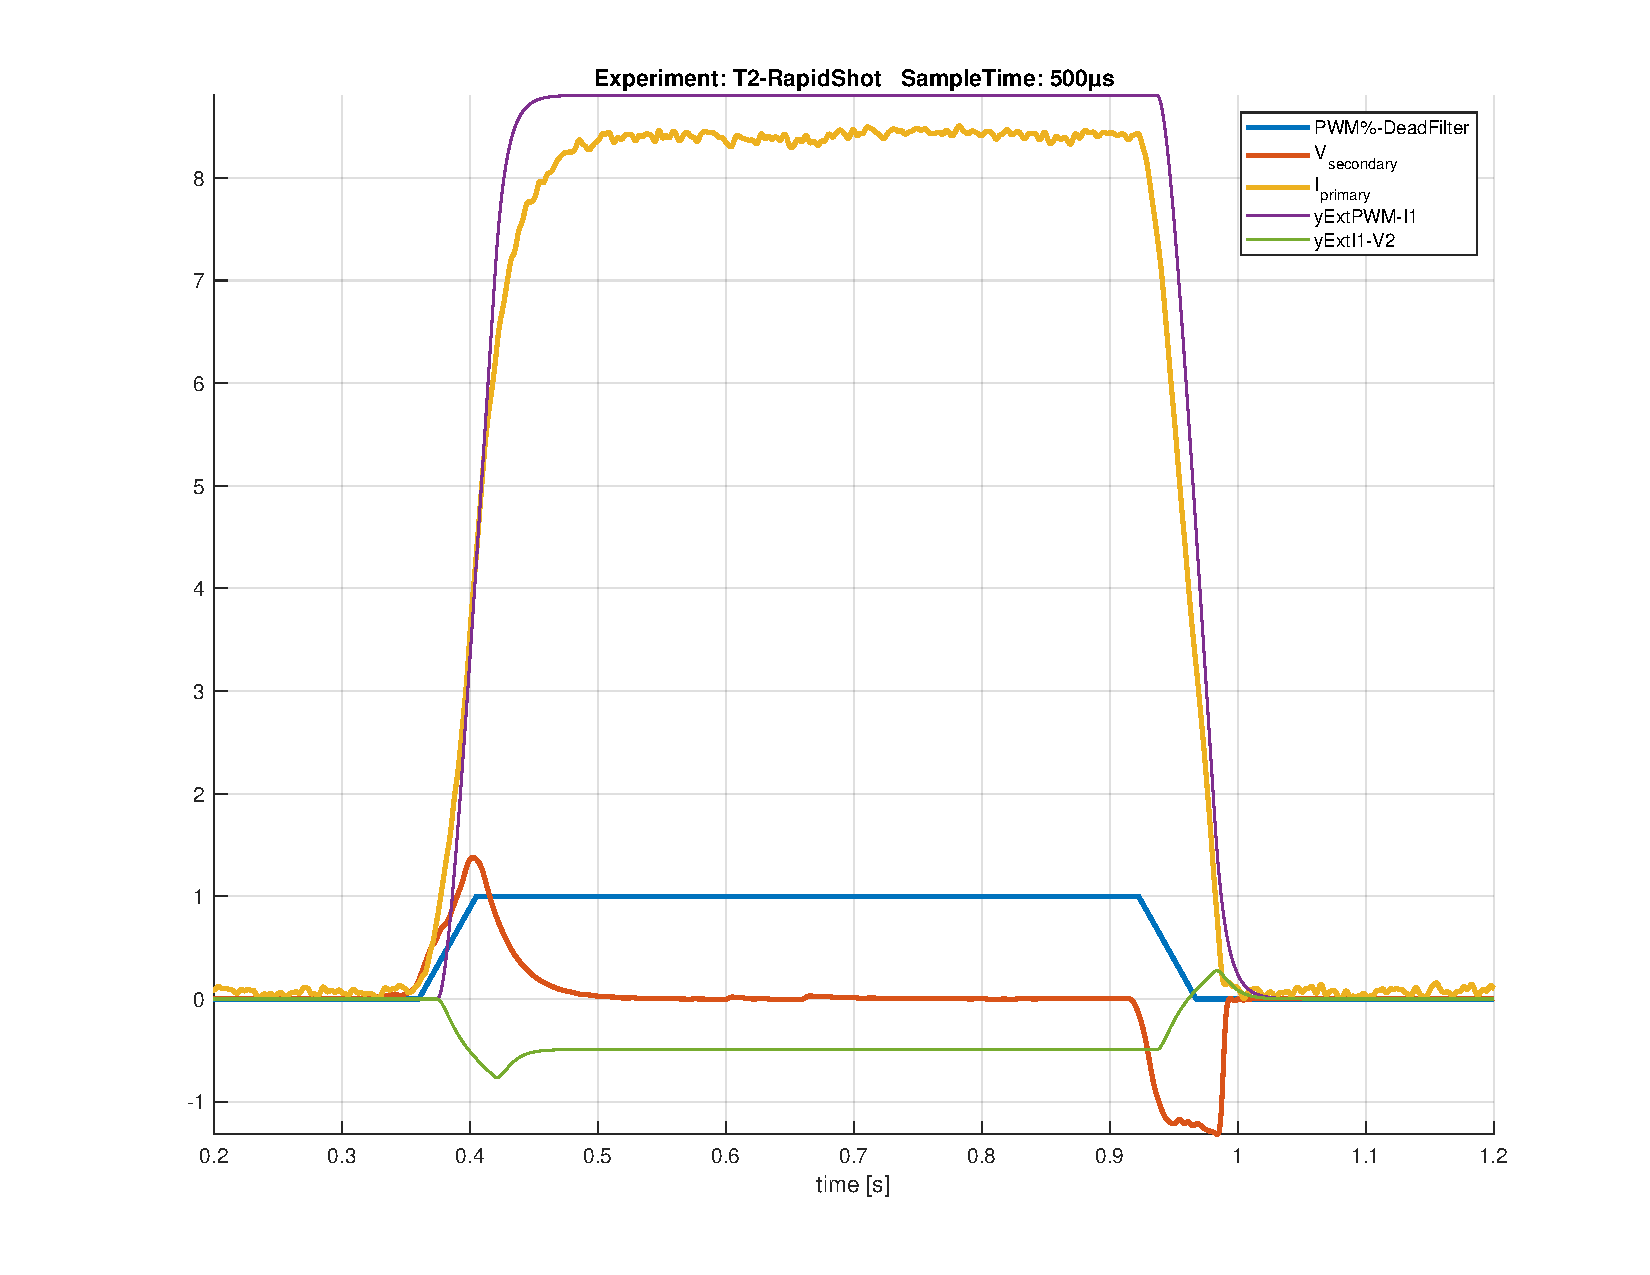
\includegraphics[width=1\textwidth]{Stime/T2-RapidShot-autoExt.pdf}
\end{figure}

\noindent
Analizzando il grafico abbiamo che i primi 3 segnali (spessi), sono i dati reali dell'esperimento filtrati (\nameref{subsec:filtraggio}), mentre le altre 2 linee rappresentano la simulazione usando la stima del Toolbox come modello.\\
Risulta facile vedere che la corrente del primario è accettabile anche se migliorabile, ma la funzione di trasferimento stimata per il secondario è completamente sbagliata, anche se dimensionalmente è simile.\\
Usando queste stime come base si sono trovati a mano dei coefficienti che meglio approssimano l'andamento delle curve.


\section{Tuning dei coefficienti}
Partendo dai modelli generati da \cite*{IdentificationToolbox} e riportati in tabella \ref{tab:stimaAutomaticaParametri}, si sono '\textit{limati}' i dati a mano per migliorare la stima dei parametri, di seguito è riportata la tabella con i valori migliorati:
\begin{table}[H]
	\centering
	\caption[Stime parametri tarati a mano]{Stime parametri tarati a mano}		\label{tab:stimaManualeParametri}
	\vspace{1mm}
	\begin{tabular}[t]{||l|c|c||}
		\hline
		\multicolumn{1}{||c}{\textbf{Funzione}}                                                & \multicolumn{1}{|c}{\textbf{Input}} & \multicolumn{1}{|c||}{\textbf{Input}} \\
		\hline\hline
		                                                                                       &                                     &                                       \\[-3mm]
		$\tilde{P}_{p_{wm} I_1}(s) = \frac{8.4}{0.022\,s+1}$                                   & PWM                                 & $I_1$                                 \\[3mm]

		$\tilde{P}_{I_1 V_2}(s) = \frac{\num{8.5e-3}\,s}{\num{3.6e-4}\,s+1}$                   & $I_1$                               & $V_2$                                 \\[3mm]

		$\tilde{P}_{p_{wm} V_2}(s) = \frac{\num{9.1e+3}\,s}{s^2+\num{2.8e+3}\,s+\num{1.3e+5}}$ & PWM                                 & $ V_2 $                               \\
		\hline
	\end{tabular}
\end{table}

\begin{figure}[H]
	\centering
	\caption[Simulazione con parametri tarati a mano]{Simulazione con parametri tarati a mano}
	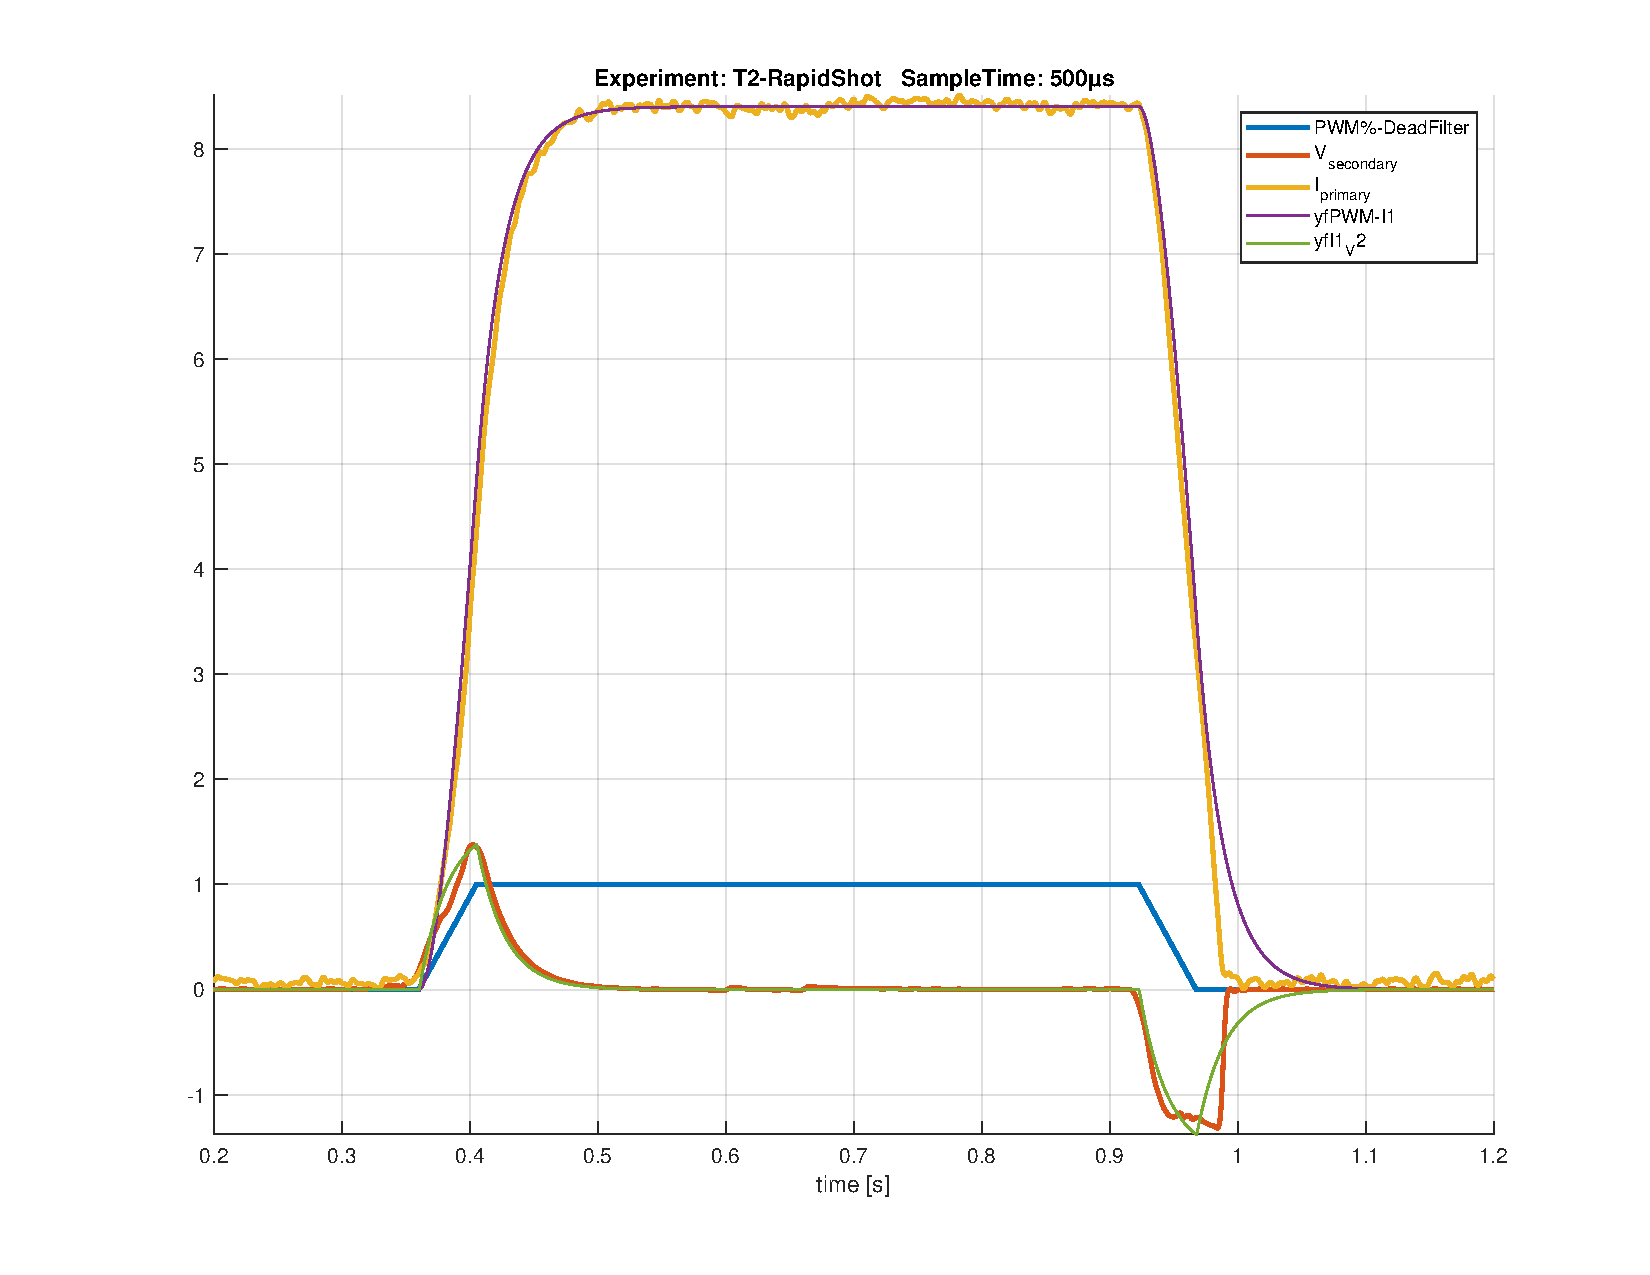
\includegraphics[width=1\textwidth]{Stime/T2-RapidShot-manualExt.pdf}
\end{figure}
\noindent
In particolare nella Dead-Zone inferiore il modello non risulta accurato, essendo predominanti le dinamiche non lineari, e ciò si vede particolarmente bene sul fronte di discesa del sistema, ma nel complesso la funzione trovata è una buona candidata per uno studio teorico e simulativo del sistema prima di passare alla fase implementativa reale.

\section{Benchmark della stima}
In questa sezione andiamo testare la qualità della stima ottenuta dando in ingresso al modello lo stesso input di un segnale eterogeneo con varie forme d'onda.\\
Metteremo quindi a confronto l'andamento reale con quello simulato preso in alcune frazioni interessanti.
\begin{figure}[H]
	\centering
	\caption[Esperimento di verifica della stima 1]{Esperimento di verifica della stima 1}
	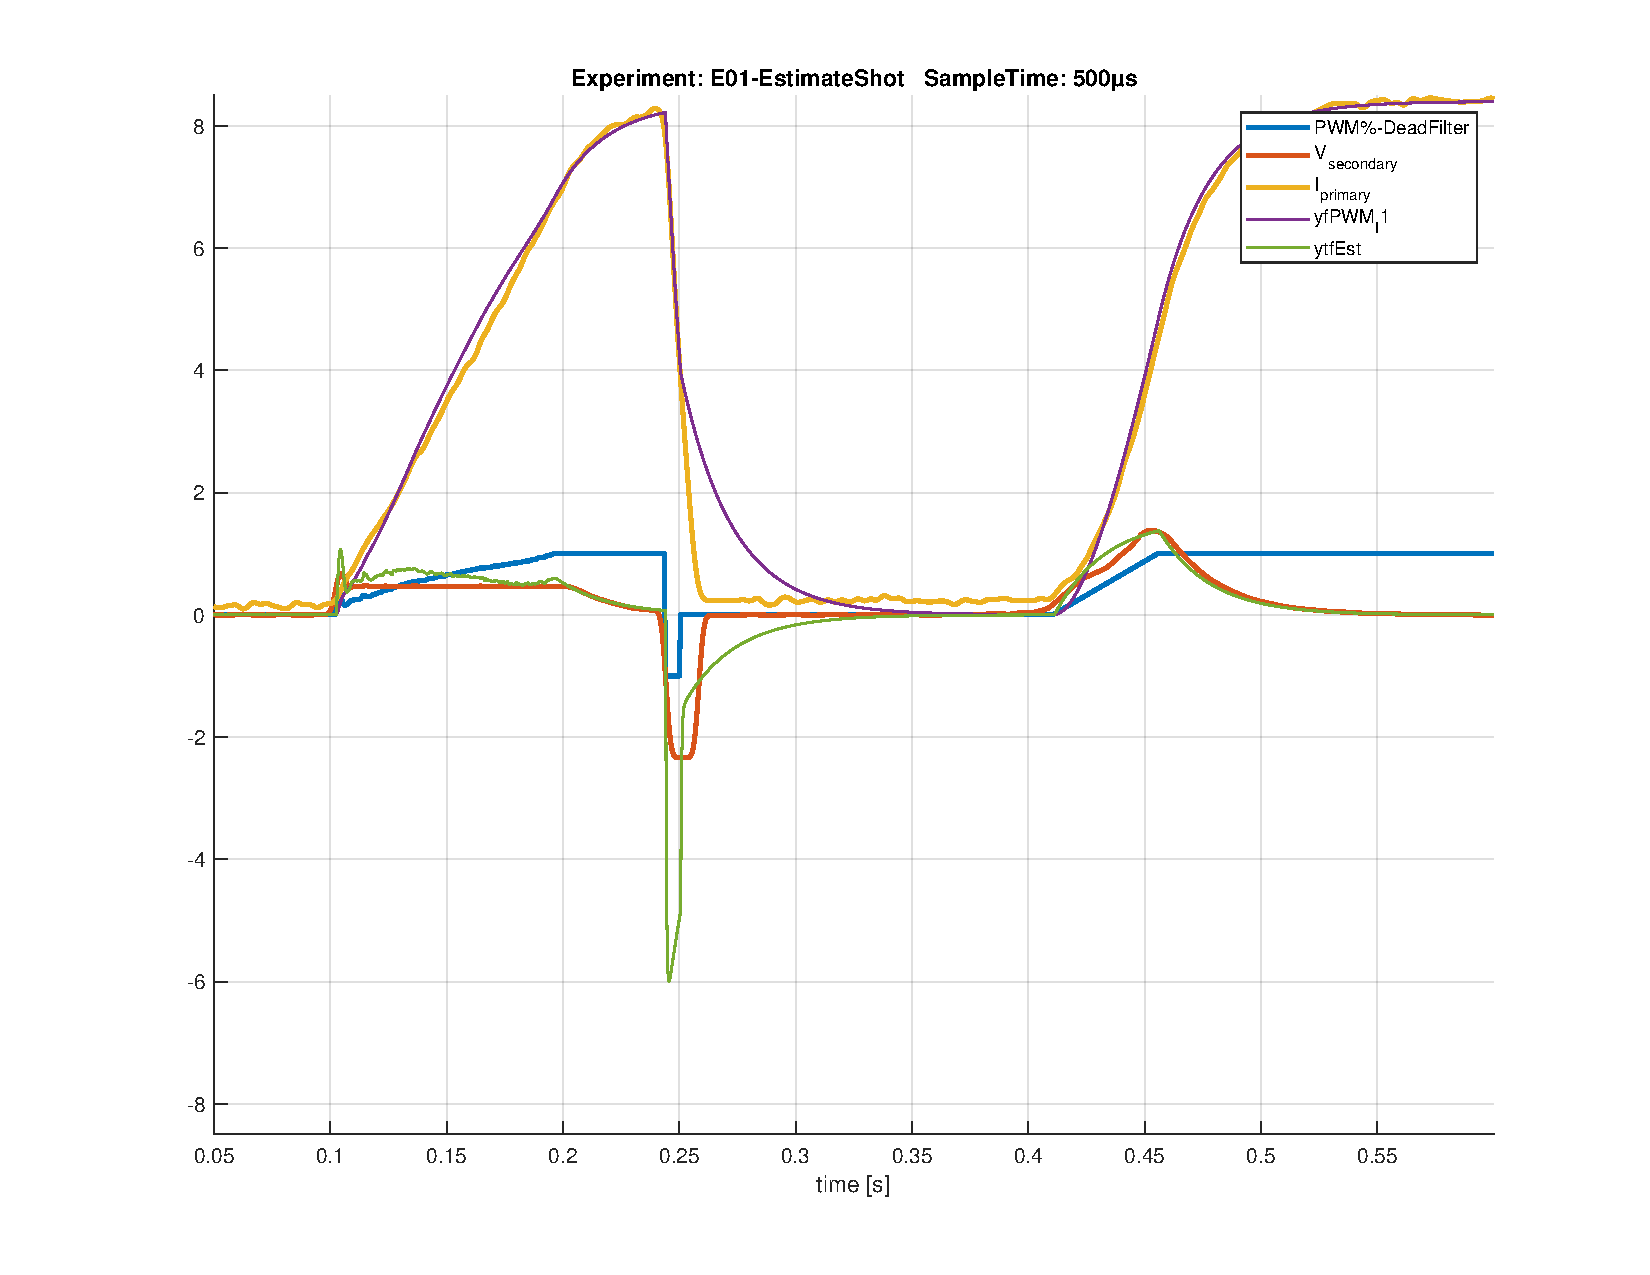
\includegraphics[width=0.9\textwidth]{Stime/E01-EstimateShot-manual-1.pdf}
\end{figure}

\begin{figure}[H]
	\centering
	\caption[Esperimento di verifica della stima 2]{Esperimento di verifica della stima 2}
	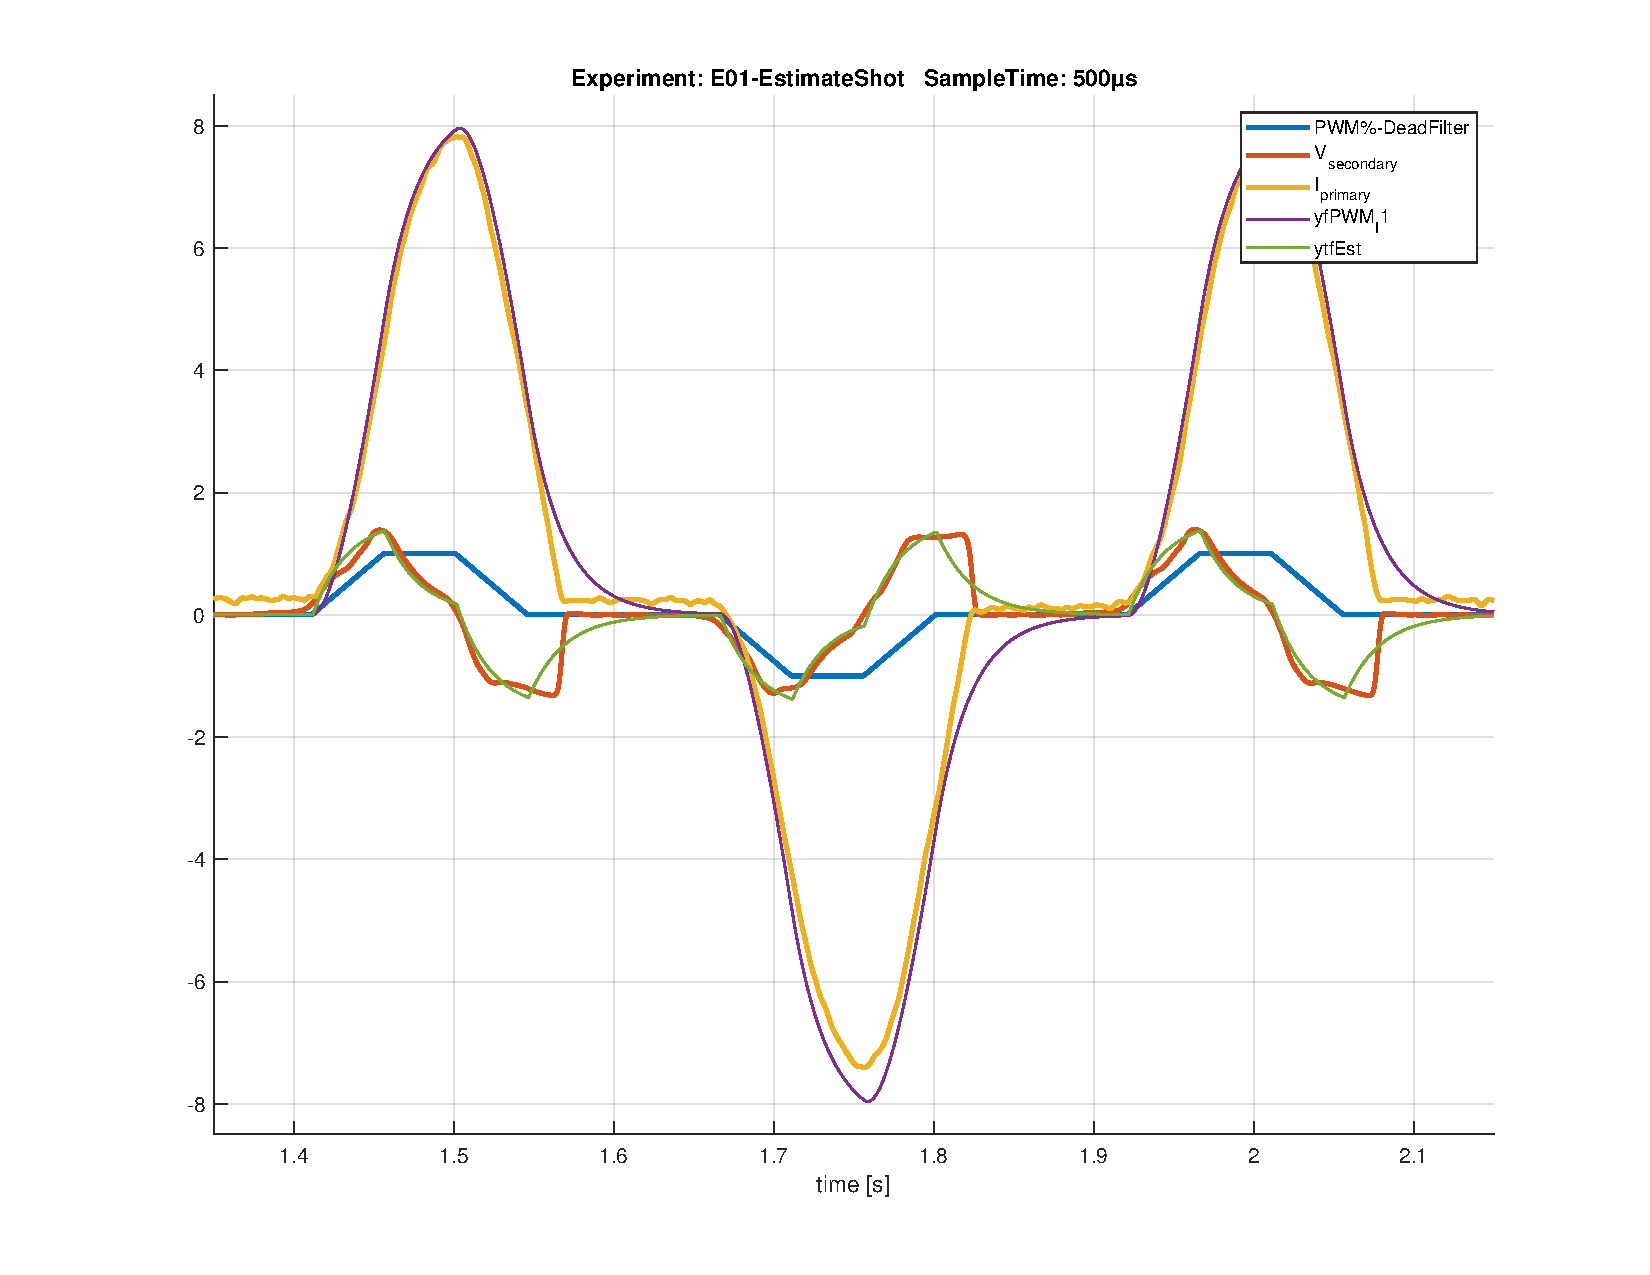
\includegraphics[width=0.9\textwidth]{Stime/E01-EstimateShot-manual-2.pdf}
\end{figure}
\vspace{-18mm}
\begin{figure}[H]
	\centering
	\caption[Esperimento di verifica della stima 3]{Esperimento di verifica della stima 3}
	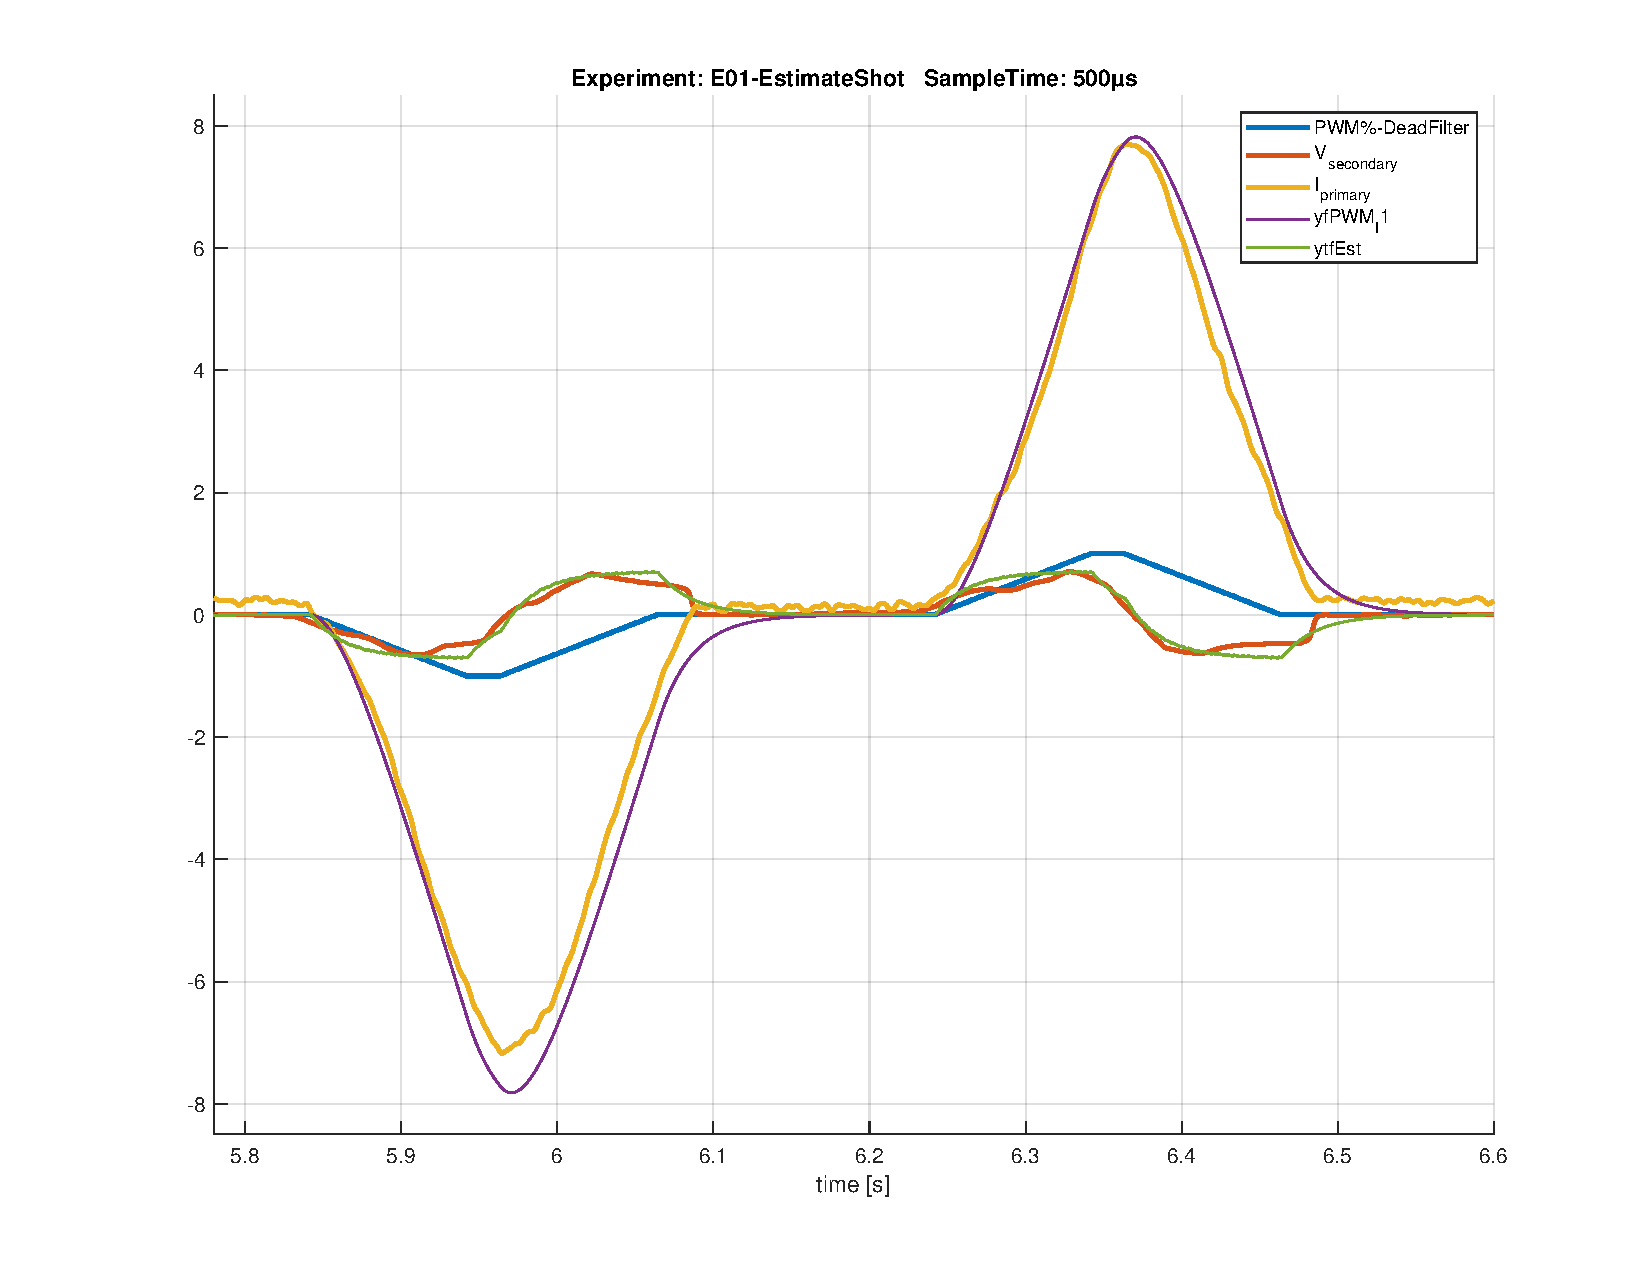
\includegraphics[width=0.9\textwidth]{Stime/E01-EstimateShot-manual-3.pdf}
\end{figure}
\noindent
Dall'analisi di questi grafici risulta chiaro che anche se il modello non è perfettamente allineato con le misure reali, a causa delle \nonLinearita del sistema originale che sono state trascurate nella creazione del modello, la dinamica simulata è rappresentativa dell'andamento reale del sistema complessivo, ed può quindi essere usata nello sviluppo teorico del controllore.\\
La funzione di trasferimento del sistema tra il segnale di PWM e arrivando alla tensione $ V_2 $ è:

\begin{Large}
	\begin{empheq}[box=\mathResult]{equation} \label{eq:StimaModelloInOut}
			\tilde{P}_{p_{wm} V_2}(s) = \frac{\num{9.1e+3}\,s}{s^2+\num{2.8e+3}\,s+\num{1.3e+5}}
	\end{empheq}
\end{Large}

\noindent
Nel seguito della tesi, questa funzione di trasferimento, con questi coefficienti, verrà usata nelle simulazioni del controllore, e ci permetterà di avere un idea qualitativa di come si comporterà il controllo una volta implementato nella realtà.\\
Come potevamo aspettarci dall'analisi teorica, i poli di $ \tilde{P}_{p_{wm} V_2} $ sono:
\begin{itemize}
	\item $ s\approx-2752.77 $
	\item $ s\approx-47.2251 $
\end{itemize}
\noindent
Il ché, come ci aspettavamo dalla teoria visto nella sezione '\nameref{TrasformatoreModelloTokamak}', fa si che il sistema sia Asintoticamente Stabile poiché i poli appartengono entrambi a $ \mathbb{C}^- $, e nel caso particolare sono 2 poli semplici, il ché, anche se probabile, non era scontato.






\chapter{Modello teorico di Controllo}\label{cap:controlModel}

\begin{minipage}{12cm}\textit{Se lo si desidera, utilizzare questo spazio per inserire un breve riassunto di ci\`o che verr\`a detto in questo capitolo. Inserire solo i punti salienti.}
\end{minipage}

\vspace*{1cm}

\section{Obiettivo di controllo}
Come accennato nella sezione "\nameref{sub:parametriMisurati}", attraverso il controllo e attuazione della corrente nel Primario del trasformatore, si punta controllare la corrente presente sul primario del trasformatore, e sempre come detto nella sezione "\nameref{sub:parametriMisurati}", non essendo possibile misurare la corrente di plasma direttamente, si usa la sua misura indiretta che passa per la $ F_{em} $.\\
In questa tesi l'obiettivo che ci si è ripromessi di raggiungere è la creazione di un controllo ad errore nullo sulla corrente di plasma.\vspace{-4mm}
\begin{figure}[H]
	\centering
	\caption[Sistema da controllare a blocchi con $ P(s) $]{Sistema da controllare a blocchi con $ P(s) $}
	\vspace{1mm}
	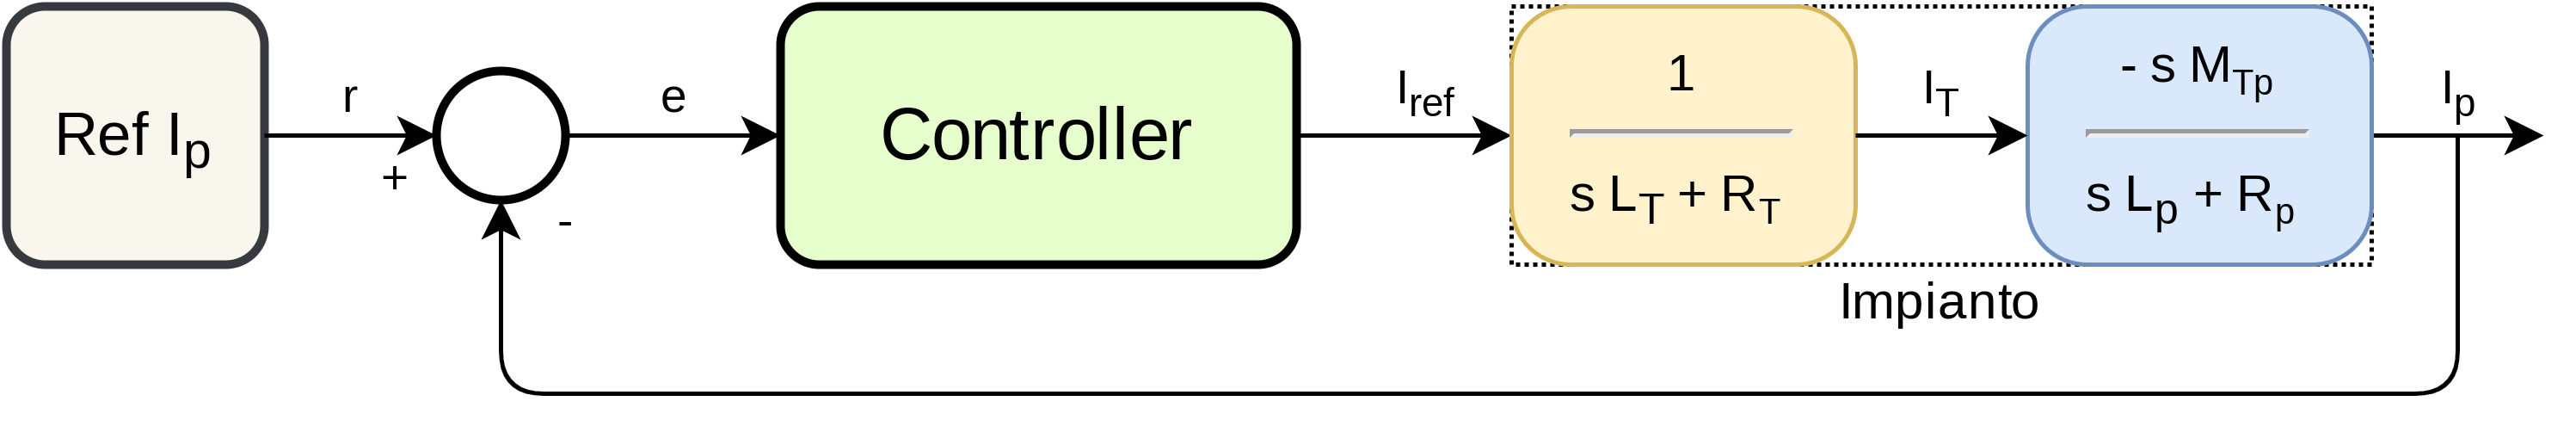
\includegraphics[width=1\textwidth]{ModelloMatematico/SchemiBlocchi.png}
\end{figure}\vspace{-4mm}

\noindent
Come visto però nella sezione, "\nameref{sub:parametriMisurati}", la misura a nostra disposizione il voltmetro la $V_2$, che equivale alla  diagnostica di $ V_{loop} $ in un impianto reale.\\
Dall'equazione della dinamica del plasma \ref{eq:correntePlasmaDinamica} siamo in grado di ricavare che:
\begin{empheq}[box=\mathStep]{equation*}
	V_2 = I_p \cdot R_p = F_{em} - L_p \cdot \dot{I_p}
\end{empheq}

\noindent
La quale, trascurando la dinamica del filtro RC di misura (che comunque è $ >= f_{tic} $ di acquisizione e di conseguenza ha una dinamica estremamente più rapida del segnale da misurare)  permette di ricavare, invertendo il segno della tensione come della corrente per avere i segni positivi, la funzione di ingresso-uscita dalla $ I_{ref} $ alla $ V_2 $ pari a:
\begin{empheq}[box=\mathCalc]{equation}
	V_2(s) = I_p(s) \cdot- R_p \Rightarrow V_2(s) = P_{pos}(s) \cdot I_{ref}(s) \cdot R_p
\end{empheq}
Da cui la funzione di trasferimento complessiva diventa:
\begin{empheq}[box=\mathCalc]{equation}\label{eq:FunxTrasImpiantoIrefV2}
	\frac{V_2(s)}{I_{ref}(s)} = P_{pos}(s) \cdot R_p
\end{empheq}
E il riferimento di corrente di plasma, diventa un riferimento di tensione secondo l'equazione di conversione:
\begin{empheq}[box=\mathCalc]{equation}\label{eq:V2RefEquivalent}
	V_{2_{ref}} = I_{p_{ref}} \cdot R_p
\end{empheq}

\begin{figure}[H]
	\centering
	\caption[Sistema da controllare ingresso-uscita reale]{Sistema da controllare ingresso-uscita reale}
	\vspace{1mm}
	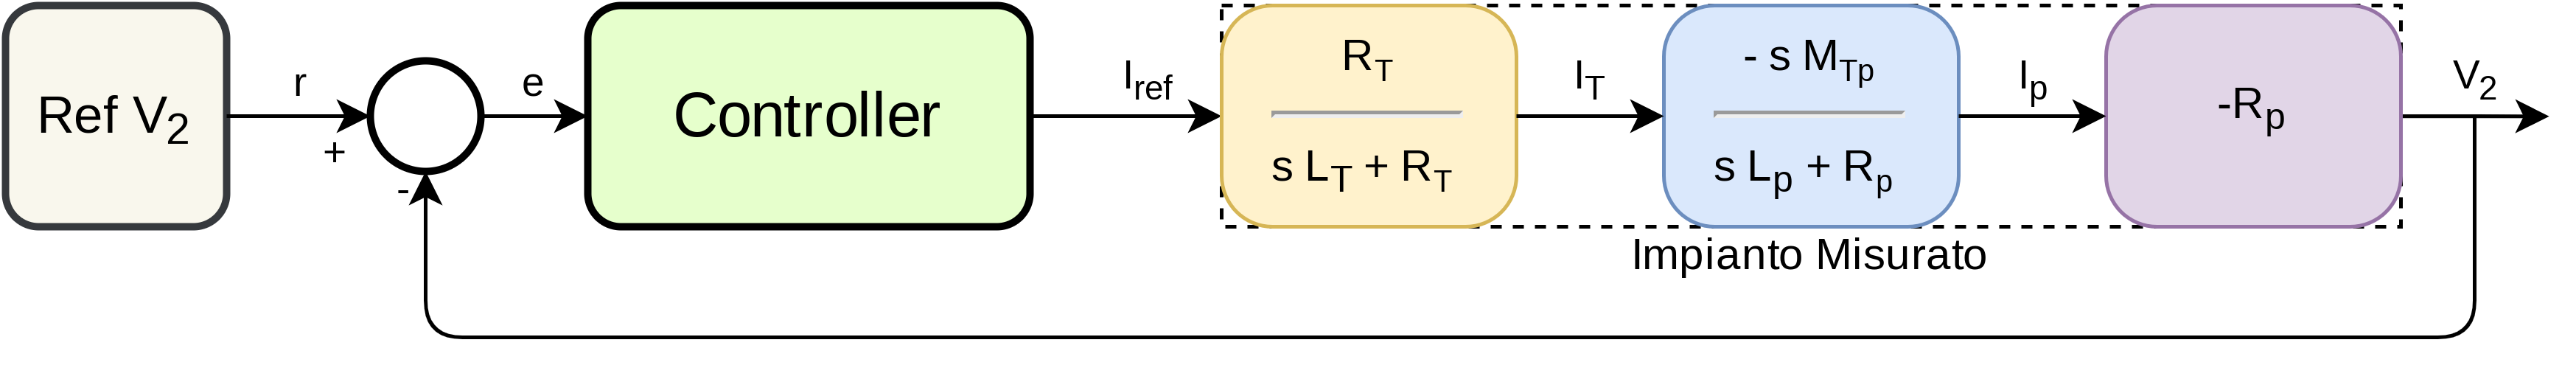
\includegraphics[width=1\textwidth]{ModelloMatematico/SchemiBlocchi-SchemaBlocchiV2Out.png}
\end{figure}

\newpage
\section{Teorema del valore iniziale e del valore finale}
Prima di procedere con il calcolo del controllore per i nostri scopi, è bene ricordare il \nameref{th:valIniziale} e il \nameref{th:valFinale} della Trasformata di Laplace (\cite*{Laplace}):

\begin{teorema}[Teorema del valore iniziale \label{th:valIniziale}]
	Se una funzione reale $ f  $ ha trasformata razionale $ F(s) $ con grado del denominatore maggiore del grado del numeratore (vale comunque sotto ipotesi ancora più larghe , purché $ F $ sia non razionale e $ f(0^+) $ esista) allora:
	\begin{empheq}[box=\mathResult]{equation} \label{eq:valIniziale}
		f(0^+) = \lim\limits_{s \rightarrowtail \infty} s \cdot F(s)
	\end{empheq}
\end{teorema}

\begin{teorema}[Teorema del valore finale \label{th:valFinale}]
	Se una funzione reale $ f  $ ha trasformata razionale $ F(s) $ con grado del denominatore maggiore del grado del numeratore e \underline{radici del denominatore (\textbf{poli}) nell’origine e o a parte reale negativa},\\
	allora:
	\begin{empheq}[box=\mathResult]{equation} \label{eq:valFinale}
		\lim\limits_{t \rightarrowtail \infty} f(t) = \lim\limits_{s \rightarrowtail 0} s \cdot F(s)
	\end{empheq}
\end{teorema}

Questi 2 Teoremi chiave, permettono di risolvere comodamente le equazioni differenziali, e quindi calcolare in maniera semplice il controllore che permette di ottenere gli obiettivi di controllo che ci si è prefissati di ottenere.

\newpage

\section{Controllo a errore nullo} \label{sec:inseguitoreErroreNullo}
\vspace{-5mm}
Definiamo ora $ P_m(s) $ come l'impianto Reale misurato tra la corrente di riferimento $ I_{ref} $ del primario, e la tensione del campo elettrico $ V_2 $ sul secondario.\\
Ne segue che la funzione di trasferimento complessiva è pari a:
\begin{empheq}[box=\mathCalc]{equation}\label{eq:impiantoMisurato}
	P_m(s)= \frac{V_2(s)}{I_{ref}(s)} = \frac{s M_{Tp} \cdot R_p}{( s L_p + R_p)(s L_T + R_T)} = \frac{s M_{Tp} \cdot R_p}{s^ 2L_p L_T + s(L_p R_T + L_T R_p) + R_p R_T}
\end{empheq}
Essendo il nostro obiettivo quello di portare $ e \rightarrowtail 0$ per $ t\rightarrowtail \infty $ con riferimenti $ r = cost $, ci calcoliamo la funzione sensitività $ W_{er}(s) $ (\textit{sensitivity transfer function}) e con il \nameref{th:valFinale} progetteremo il controllore $ C(s) $ che realizza l'obiettivo:\\
\begin{vwcol}[widths={0.5,0.5}, sep=8mm, rule=0px]
	\vspace{-12mm}
	\begin{empheq}[box=\mathStep]{equation*}
		W_{er}(s) = \frac{e(s)}{r(s)} = \frac{1}{1 + P_m(s)C(s)}
	\end{empheq}
	\newpage
	{\color{red} Sensitivity transfer function}\\[-6mm]
	{\footnotesize (\cite{PerfAndRobust})}
\end{vwcol}
\vspace{5mm}
\begin{vwcol}[widths={0.5,0.5}, sep=8mm, rule=0px]
	\vspace{-8mm}
	\begin{empheq}[box=\mathStep]{equation*}
		r(t) = cost \rightarrow r(s)= \frac{K_r}{s}
	\end{empheq}
	\newpage
	Trasformata di Laplace del riferimento
\end{vwcol}\vspace{-3mm}
\noindent
Da cui, applicando il \nameref{th:valFinale} otteniamo:
\begin{empheq}[box=\mathCalc]{equation} \label{eq:dinamicaErroreRifCostFunxTrasf}
	\lim\limits_{t \rightarrowtail \infty} e(t) = \lim\limits_{s \rightarrowtail 0} s \cdot W_{er}(s) \cdot r(s) = s \cdot \frac{K_r / s}{1 + P_m(s)C(s)}
\end{empheq}

\begin{oss} \label{oss:Fattorizzazione}
	Al fine di semplificare il design del controllore, fattorizziamo ora $ P_m(s) $ e $ C(s) $ nella seguente forma, tralasciando così i dettagli dei termini non utili ai fini del design del controllore.\\[0mm]
	\begin{vwcol}[widths={9cm,4cm}, sep=0mm, rule=0px]
		\vspace{-8mm}
		\begin{empheq}[box=\mathStep]{equation*}
			C(s) = K_c \cdot \frac{s^{\rho_{c_n}} \cdot \prod_{i=1}^{\#Zeri\neq0} \left ( \frac{s}{z_i} + 1 \right )}{s^{\rho_{c_d}} \cdot \prod_{i=1}^{\#Zeri\neq0} \left ( \frac{s}{p_i} + 1 \right )} = 
			\frac{K_c}{s^{\rho_{c}}} \cdot \frac{C_n(s)}{C_d(s)}
		\end{empheq}
		\newpage
		\begin{spacing}{1.25}
			{\scriptsize
				\begin{itemize}[itemsep=-1mm,leftmargin=6mm]
					\item $ K_c $ Guadagno statico Controllore.
					\item $ C_n $ Polinomio numeratore \underline{senza Zeri in 0}.
					\item $ C_d $ Polinomio denominatore \underline{senza Poli 0}.
					\item $ \rho_c $ è il grado del polo in 0 ($ \rho_{c_d} - \rho_{c_n} $).
				\end{itemize}
			}
		\end{spacing}
	\end{vwcol}
	
	\noindent\rule[0.5ex]{\linewidth}{0.5pt}\\[0mm]
	
	\begin{vwcol}[widths={9cm,4cm}, sep=0mm, rule=0px]
		\vspace{-10mm}
		\begin{empheq}[box=\mathStep]{equation*}
						P(s) = K_p \cdot \frac{s^{\rho_{p_n}} \cdot \prod_{i=1}^{\#Zeri\neq0} \left ( \frac{s}{z_i} + 1 \right )}{s^{\rho_{p_d}} \cdot \prod_{i=1}^{\#Zeri\neq0} \left ( \frac{s}{p_i} + 1 \right )} = 
			\frac{K_p}{s^{\rho_{p}}} \cdot \frac{P_n(s)}{P_d(s)}
		\end{empheq}
		\newpage
		\begin{spacing}{1.25}
			{\scriptsize
				\begin{itemize}[itemsep=-1mm,leftmargin=6mm]
					\item $ K_p $ Guadagno statico Impianto.
					\item $ P_n $ Polinomio numeratore \underline{senza Zeri in 0}.
					\item $ P_d $ Polinomio denominatore \underline{senza Poli 0}.
					\item $ \rho_p $ è il grado del polo in 0 ($ \rho_{p_d} - \rho_{p_n} $).
				\end{itemize}
			}
		\end{spacing}
	\end{vwcol}
\end{oss}
\newpage
Partendo da questa forma, svolgiamo i calcoli dell'equazione  \ref{eq:dinamicaErroreRifCostFunxTrasf}:
\begin{empheq}[box=\mathCalc]{equation} \label{eq:guadagnoAnelloPlusOne}
			1 + P_m(s)C(s) =  1 + \frac{K_c}{s^{\rho_{c}}} \frac{C_n}{C_d}\cdot \frac{K_p}{s^{\rho_{p}}}  \frac{P_n}{P_d}=
			\frac{s^{\rho_{c} + \rho_{p}} C_d P_d + K_c K_p C_n P_n}{s^{\rho_{c} + \rho_{p}} C_d P_d}
\end{empheq}

Da cui otteniamo che:
\begin{center}
	{\large
		$ s \cdot W_{er}(s) \cdot r(s) =
			\cancel{s} \cdot \frac{K_r/\cancel{s}}{1 + P_m(s)C(s)} =
			K_r \cdot \left(\frac{s^{\rho_{c} + \rho_{p}} C_d P_d + K_c K_p C_n P_n}{s^{\rho_{c} + \rho_{p}} C_d P_d}\right)^{-1} \Rightarrow$
	}
\end{center}

\begin{empheq}[box=\mathStep]{equation*}
	\lim\limits_{t \rightarrowtail \infty} e(t) = \lim\limits_{s \rightarrowtail 0} s \cdot W_{er}(s) \cdot r(s) = \lim\limits_{s \rightarrowtail 0}
	K_r \cdot \frac{{\color{fireenginered}s^{\rho_{c} + \rho_{p}}} \cdot C_d P_d}{{\color{fireenginered}s^{\rho_{c} + \rho_{p}}} \cdot C_d P_d + K_c K_p C_n P_n}
\end{empheq}
Tenendo presente che $ C_d,P_d,C_n,P_n \rightarrowtail 1 $ per $ s \rightarrowtail 0 $, poiché gli Zeri sono stati fattorizzati fuori assieme al guadagno Statico (vedi osservazione \ref{oss:Fattorizzazione}), abbiamo che gli esiti per l'errore a \textit{Steady state} (Stato Stazionario) dipendono solo dal grado di {\color{fireenginered}$ \rho = \rho_{c} + \rho_{p} $ con $ \rho \in \mathbb{Z} $} e sono pari a:

\begin{center}	\label{eq:esitiErrore}
	$ e_\infty = \lim\limits_{t \rightarrowtail \infty} e(t) =
	\left \{ \begin{array}{l c c}
		0                   & se & \rho \geq 1  \\
		\frac{K_r}{K_c K_p} & se & \rho = 0     \\
		\infty                & se & \rho \leq 0 
	\end{array}
	\right.
$
\end{center}
Essendo {\color{fireenginered}$ \rho_{p} = -1 $} a causa dello Zero in 0, abbiamo che il controllore dovrà necessariamente avere {\color{fireenginered}$ \rho_{c} = 2 $} per ottenere {\color{fireenginered}$ \rho = 1 $}. Il grado minimo di controllore di cui necessitiamo è quindi:
\begin{empheq}[box=\mathStep]{equation}	\label{eq:contollerDesignBase}
	C(s) = \frac{1}{s^2}
\end{empheq}
Questo controllore base è complicabile a piacere aggiungendo altri Poli e Zeri stabili, con l'obiettivo di migliorarne le performance della risposta del sistema.
\begin{oss}
	Il controllore descritto in \ref{eq:contollerDesignBase}, anche se stabilizza il sistema e lo rende un \underline{inseguitore ad errore nullo}, \textbf{non è stabile}.\\
	Esso infatti ha 2 poli in 0, rendendolo un polo \underline{non semplice} e quindi causa di instabilità polinomiale.\\
	Questa conseguenza è inevitabile e bene accetta poiché permette di inseguire con errore nullo, per la durata dell'esperimento, il riferimento.\\
	Bisognerà ovviamente tenerne conto in fase di realizzazione poiché con il procedere del tempo dell'esperimento, i numeri dello stato diventeranno sempre maggiori, e ciò potrà portare a problemi di overflow numerici.
\end{oss}

\newpage
\noindent
La dinamica $ e_\infty $ riportata (\ref{eq:esitiErrore}) è valida $\leftrightarrow$ il sistema a ciclo chiuso $ W_{V_2 r}(s) $ risulta Asintoticamente Stabile, analizziamo quindi la sua stabilità:\\
\begin{vwcol}[widths={8cm,8cm}, sep=0mm, rule=0px]
	\vspace{-7.8mm}
	\begin{empheq}[box=\mathStep]{equation*}
		W_{V_2 r}(s) = \frac{V_2(s)}{r(s)} = \frac{P_m(s)C(s)}{1 + P_m(s)C(s)}
	\end{empheq}
	\newpage
	{\small {\color{red} Complementary Sensitivity Transfer Function}}\\[-6mm]
	{\footnotesize (\cite{PerfAndRobust})}
\end{vwcol}
\noindent
E la stabilità di questa funzione è data dai poli del suo denominatore, che abbiamo già calcolato \ref{eq:guadagnoAnelloPlusOne}, e la cui formula è:

\begin{center}
	{\large $ Den(W_{V_2 r}) = {\color{fireenginered}s^{\rho_{c} + \rho_{p}}} C_d P_d = {\color{fireenginered}s^{\rho}} C_d P_d$} \hspace{8mm} ($ C_d $ e $ P_d $ senza poli nell'origine \footnote{Nota Bene: $ P_d $ e $ C_d $ sono il risultato della fattorizzazione vista sopra nell'osservazione \ref{oss:Fattorizzazione}, non possono quindi esserci poli nell'origine in questi 2 termini \textbf{per costruzione}})
\end{center}
Partendo dalla conoscenza che $ P_d $ è sicuramente composta da poli stabili nel semipiano $ \mathbb{C^-} $ (vedi sezione \nameref{TrasformatoreModelloTokamak}), da cui segue che qualunque polo stabile per il controllore ($ C_d $) non destabilizza il sistema e rende valida la dinamica $ e_\infty $ riportata prima (\ref{eq:esitiErrore}), e anzi, il numeratore del controllore può tranquillamente essere instabile, se dovesse servire.

\subsection{Design di controllore adottato}
In questa tesi la forma di controllore che si è scelto di usare è la seguente:
\begin{empheq}[box=\mathCalc]{equation} \label{eq:controllerDesign}
	C(s) = \frac{K_2}{s^2} + \frac{K_1}{s} + K_p = \frac{K_2 + s K_1 + s^2 K_p}{s^2} 
\end{empheq}
\noindent
La scelta è dovuta alla sua somiglianza con un più classico PID, che in questo caso non sarebbe bastato a raggiungere le specifiche (vedi sezione \nameref{sec:inseguitoreErroreNullo}), ma come per lui, tramite un lavoro di \textit{Tuning} dei coefficienti è possibile ottenere delle buone prestazioni per il sistema a ciclo chiuso.\\
Ulteriore vantaggio di questa struttura è che permettere un semplice controllo switching, variando i coefficienti del numeratore, in base alla fase dell'esperimento.

\newpage

\section{Simulazione \textit{Qualitativa} su Simulink}
Partendo dal modello stimato che si è ottenuto nel capitolo "\nameref{cap:stimaModello}" in cui si è giunti al modello nell'equazione \ref{eq:StimaModelloInOut}, puntiamo ora a testare il controllo base che abbiamo teorizzato e successivamente la sua evoluzione "\textit{PID-style}".\\
Mostreremo prima come si comporta il controllore base \ref{eq:contollerDesignBase}, e successivamente modificheremo i parametri (mettendo anche la saturazione per una maggiore aderenza ai dati reali) e mostreremo gli effetti qualitativi sul sistema quando i coefficienti sono presenti o meno e le loro variazioni.\\
Di seguito i 2 sistemi di controllo usati su Simulink per generare la simulazione:
\begin{figure}[H]
	\centering
	\caption[Modelli simulati su Simulink]{Modelli simulati su Simulink}
	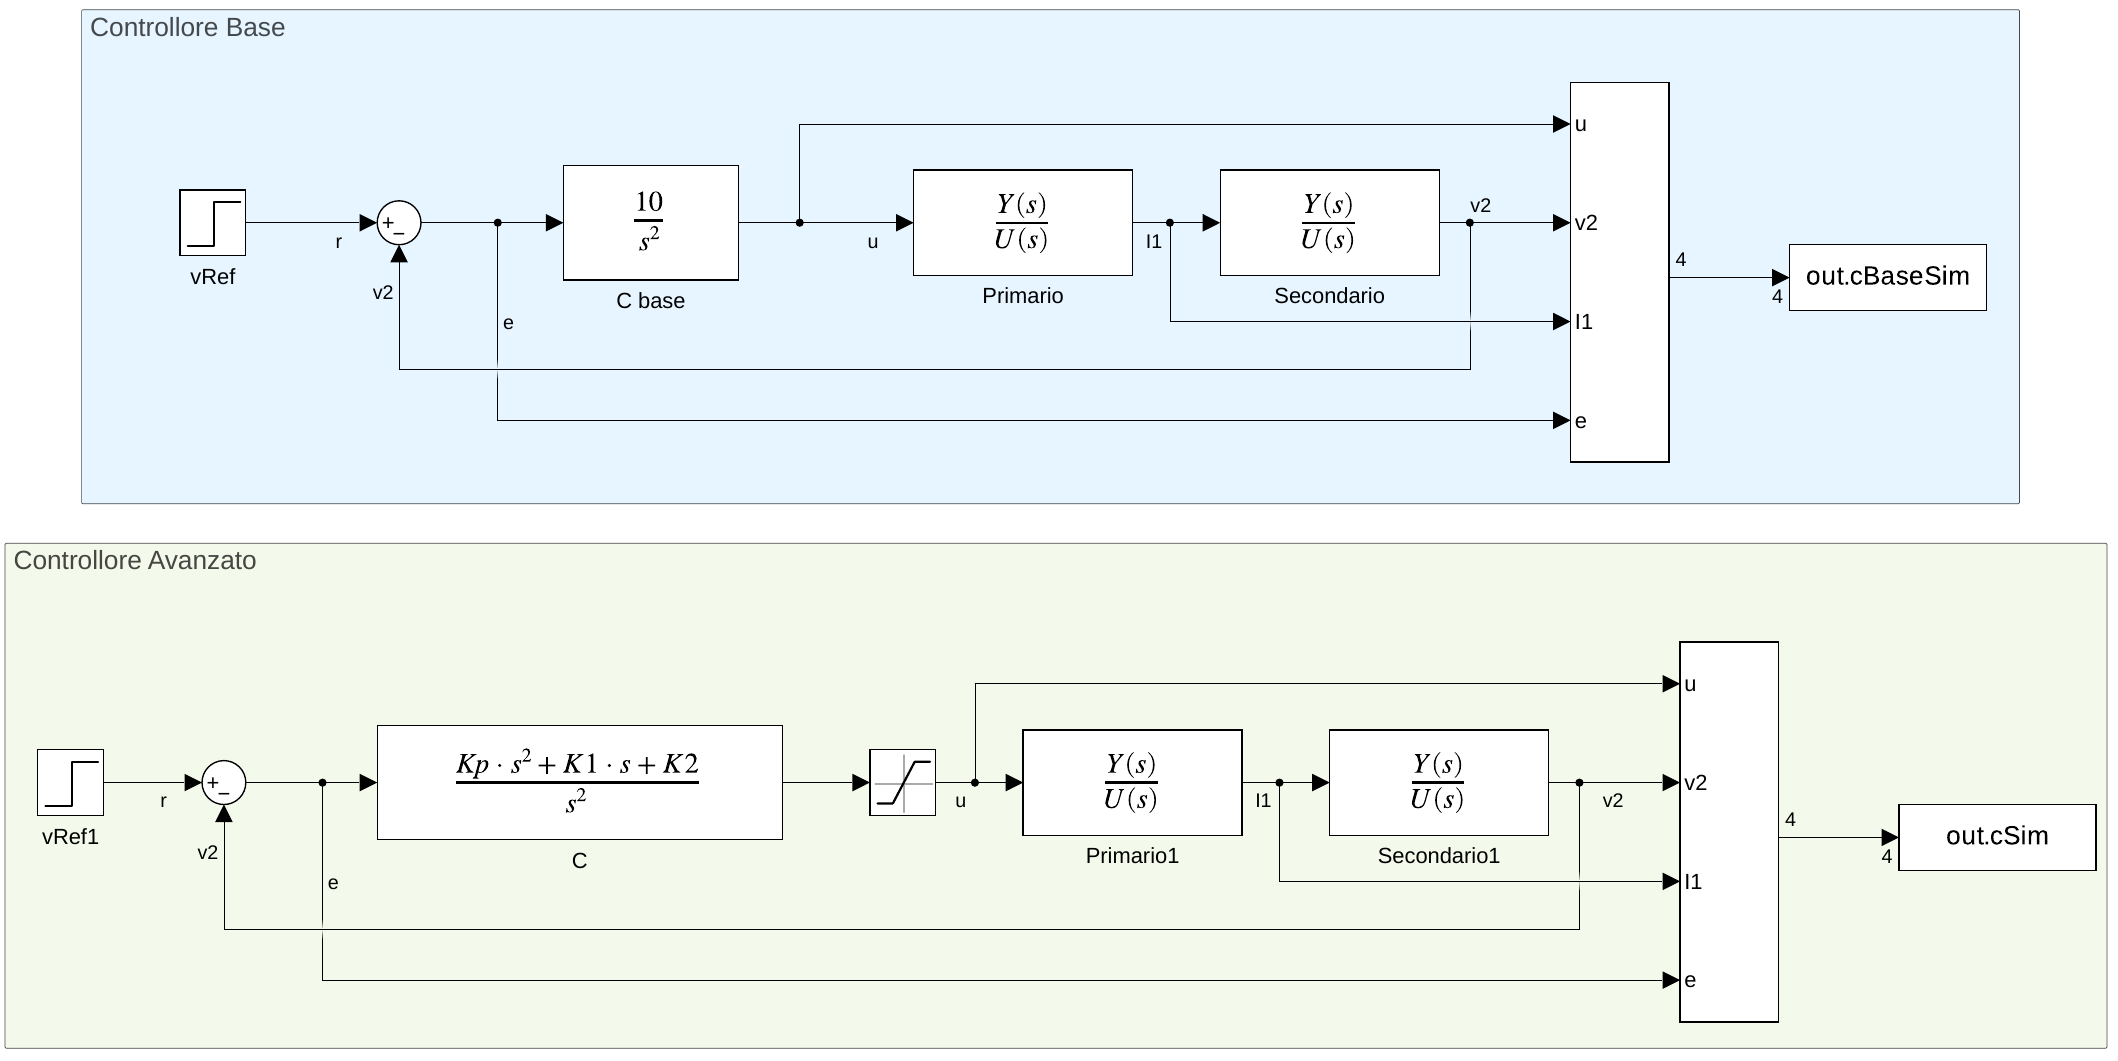
\includegraphics[width=1\textwidth]{ModelloMatematico/systemSimulink.png}
\end{figure}

\noindent
Il primo ci serve solo per mostrare l'andamento del sistema con un controllo che punta solo a ottenere gli obiettivi di controllo.\\
Al contrario il secondo punta ad analizzare la risposta del sistema al variare dei coefficienti con lo scopo preciso di migliorarne le prestazioni.
In entrambi i casi, la tensione $ V_{2_{ref}} = 0.5V$ 

\noindent
{\footnotesize NOTA BENE: I grafici riportati hanno il \textbf{\underline{segnale di errore è zoomato di un fattore 10}} per meglio mettere in evidenza il comportamento dell'errore}

\newpage

\subsection{Design Base di controllo}
Usando il controllo base e senza saturazione, abbiamo una risposta che conferma i gli esiti calcolati per $ e_\infty $ nella sezione \ref{eq:esitiErrore}:
\begin{figure}[H]
	\centering
	\caption[Modelli simulati su Simulink]{Modelli simulati su Simulink}
	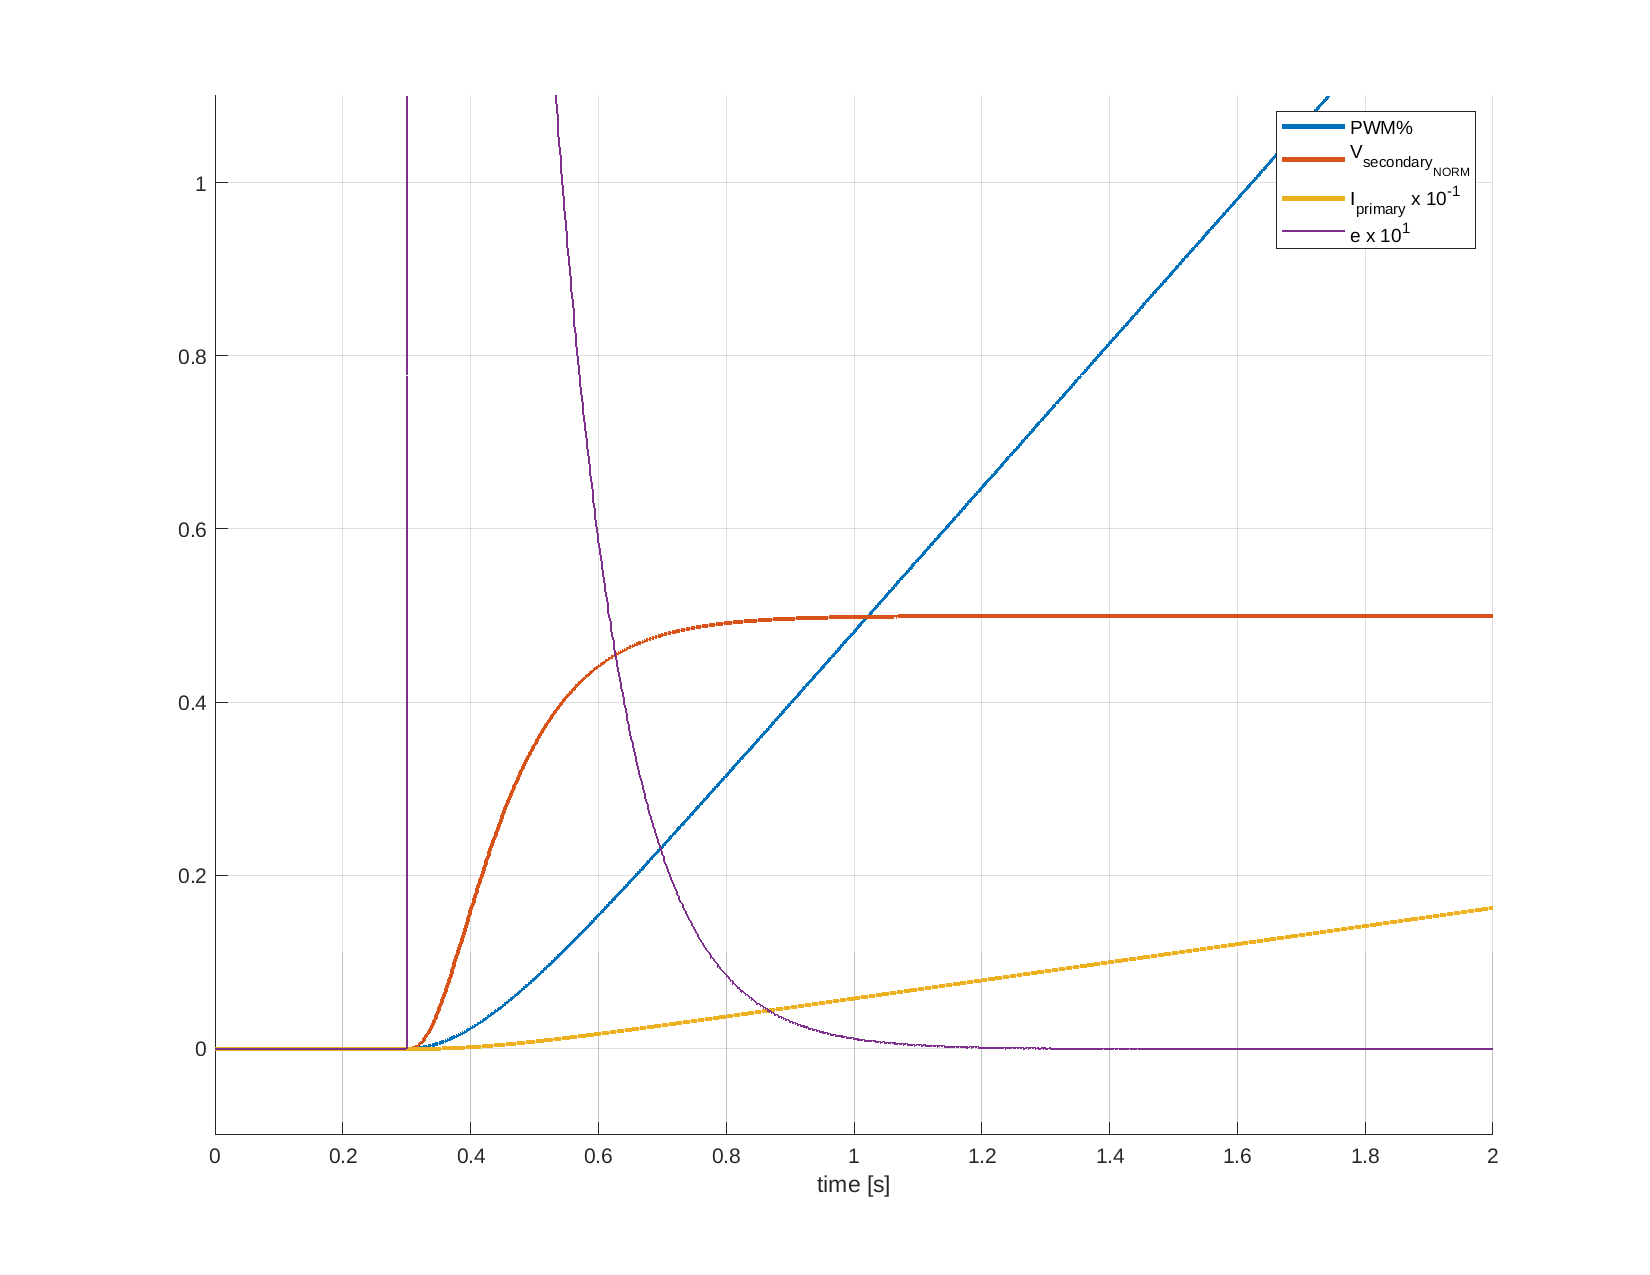
\includegraphics[width=1\textwidth]{ModelloMatematico/Simulation-cBaseSim.png}
\end{figure}

\noindent
Queste performance possono e devono essere ampliamene migliorate poiché raggiunta la saturazione del controllo, l'errore ricomincia subito a crescere ed è impossibile riprenderlo senza resettare l'esperimento.\\
In questo caso però la saturazione è stata eliminata al fine di mettere maggiormente in evidenza che asintoticamente il controllo proposto realizza le richieste di controllo di avere un inseguitore con errore nullo asintotico.

\newpage
\subsection{Design Avanzato di controllo}
Usando ora il controllore proposto nell'equazione \ref{eq:controllerDesign} analizziamo ora gli effetti della presenza dei vari termini, e il loro effetto qualitativo sulla risposta e l'andamento dell'errore.\\
Ricordiamo nuovamente che il {\color{red}\textbf{\underline{segnale di errore è zoomato di un fattore 10}}} per meglio mettere in evidenza il comportamento dell'errore.

\subsubsection{Analisi controllo Avanzato per $ K_p $=0 $ K_1 $=0 $ K_2 $=100}
\begin{figure}[H]
	\centering
	\caption[Controllo Avanzato $ K_p $=0 $ K_1 $=0 $ K_2 $=100] {Controllo Avanzato $ K_p $=0 $ K_1 $=0 $ K_2 $=100}
	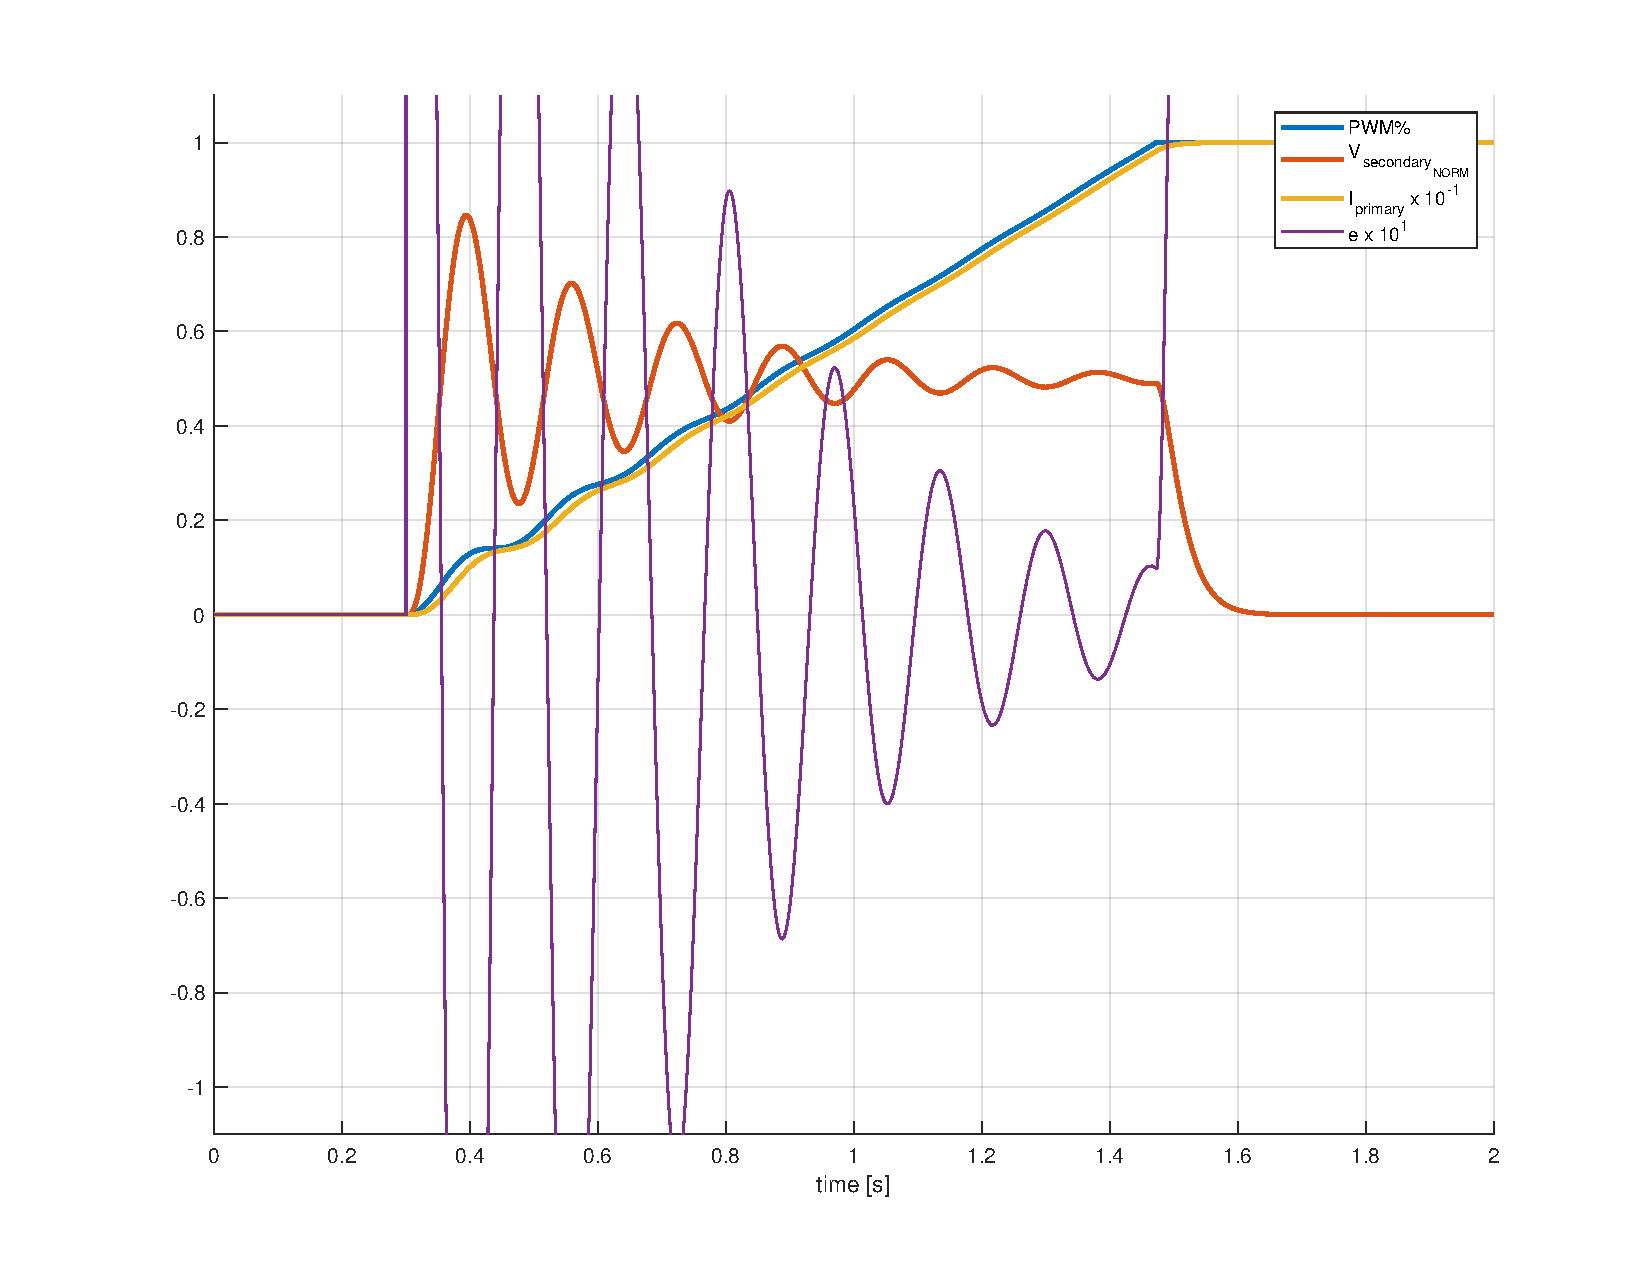
\includegraphics[width=1\textwidth]{ModelloMatematico/Simulation-cSim-Kp=0-K1=0-K2=100.pdf}
\end{figure}
\noindent
L'aumento del coefficiente per il doppio integratore ha l'effetto di creare risposte più tempestive, ma da atto a dei fenomeni oscillatori smorzati

\subsubsection{Analisi controllo Avanzato per $ K_p $=0 $ K_1 $=10 $ K_2 $=100}
In questa seconda simulazione si è aggiunto un al controllore il termine integrale:
\begin{figure}[H]
	\centering
	\caption[Controllo Avanzato $ K_p $=0 $ K_1 $=10 $ K_2 $=100]{Controllo Avanzato $ K_p $=0 $ K_1 $=10 $ K_2 $=100}
	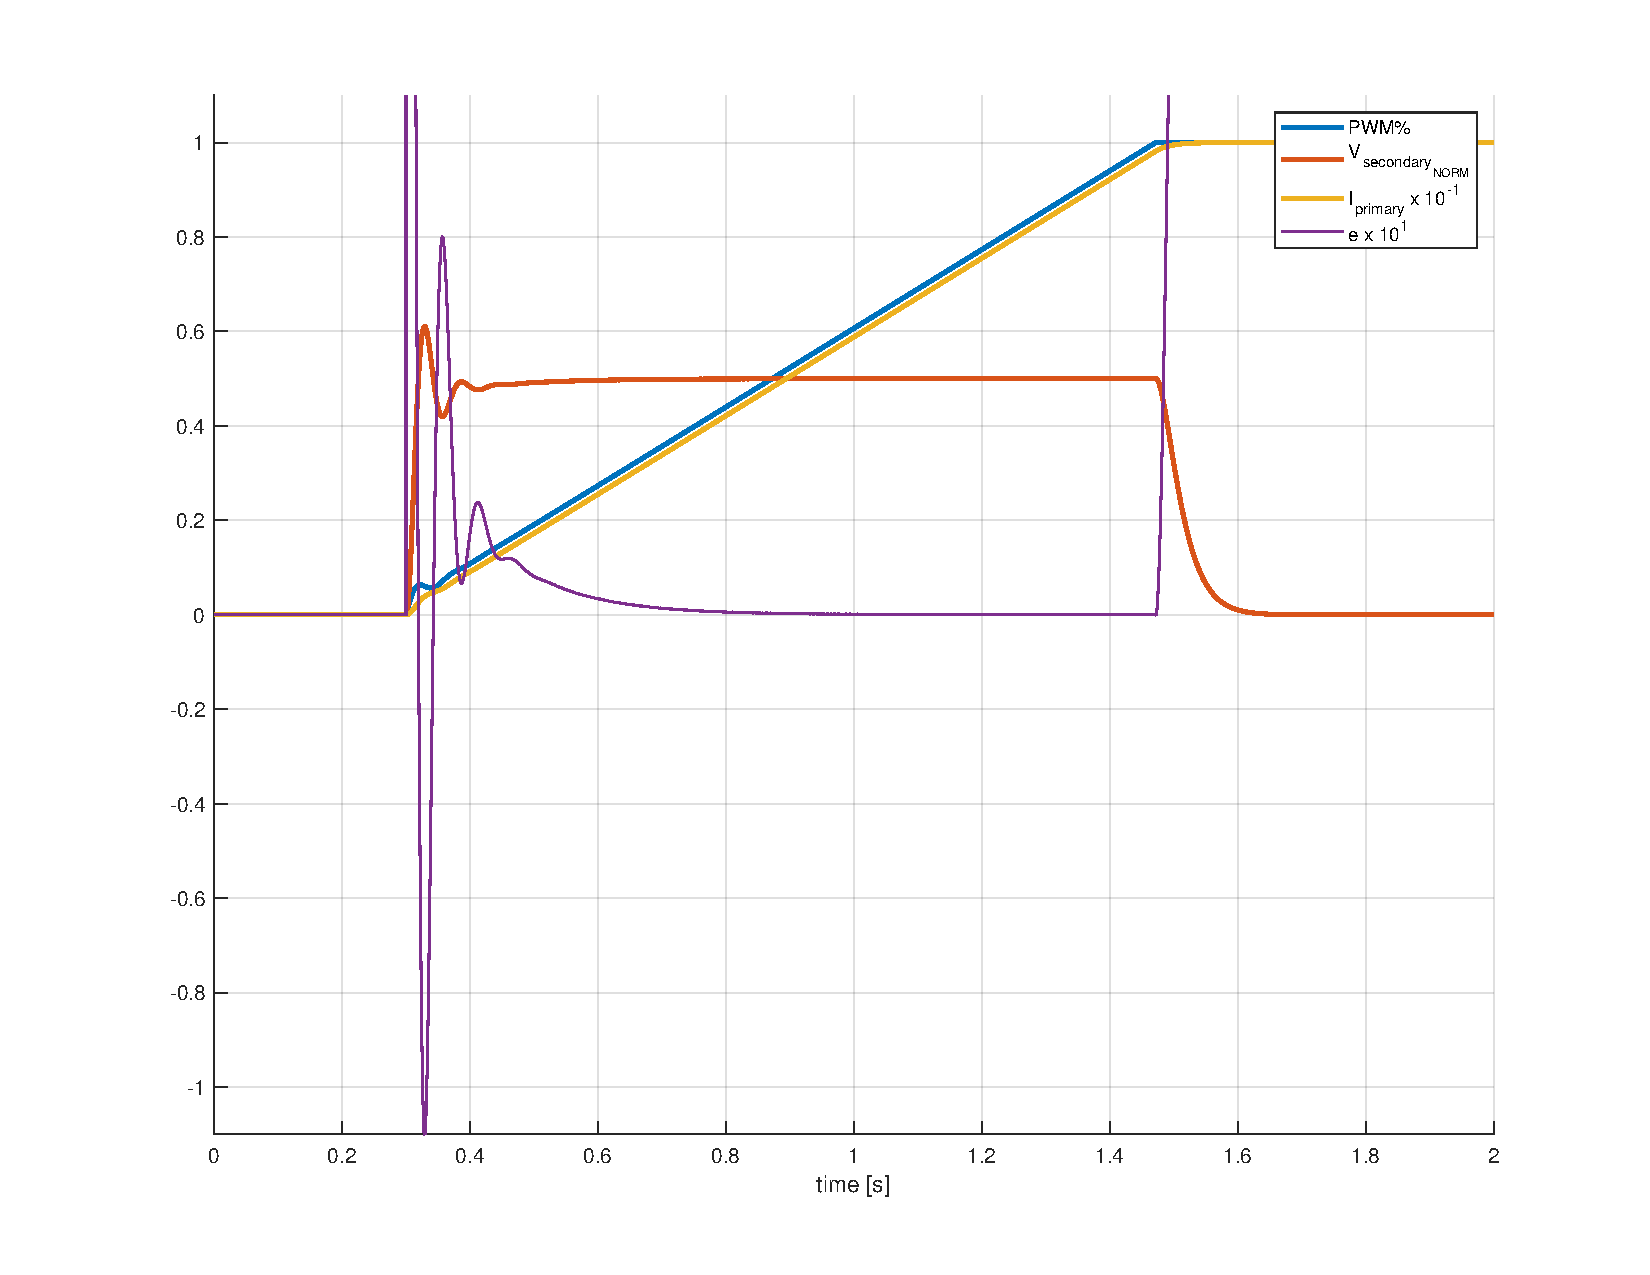
\includegraphics[width=1\textwidth]{ModelloMatematico/Simulation-cSim-Kp=0-K1=10-K2=100.pdf}
\end{figure}
\noindent
L'effetto del termine integrale è quindi smorzare il transitorio oscillatorio, per poi inseguire il riferimento con un andamento esponenziale.\\
In questo secondo esperimento abbiamo già migliorato molto le performance dal controllo base, avendo visibilmente migliorato il \underline{Tempo di assestamento} del sistema e lasciando 600ms di esperimento con errore ampiamente trascurabile.
\newpage
\subsubsection{Analisi controllo Avanzato per $ K_p $=0 $ K_1 $=100 $ K_2 $=500}
Abbiamo adesso aumentato i coefficienti del doppio e singolo integratore per vedere come migliorano le performance del sistema ad un loro aumento coordinato:
\begin{figure}[H]
	\centering
	\caption[Controllo Avanzato $ K_p $=0 $ K_1 $=100 $ K_2 $=500]{Controllo Avanzato $ K_p $=0 $ K_1 $=100 $ K_2 $=500}
	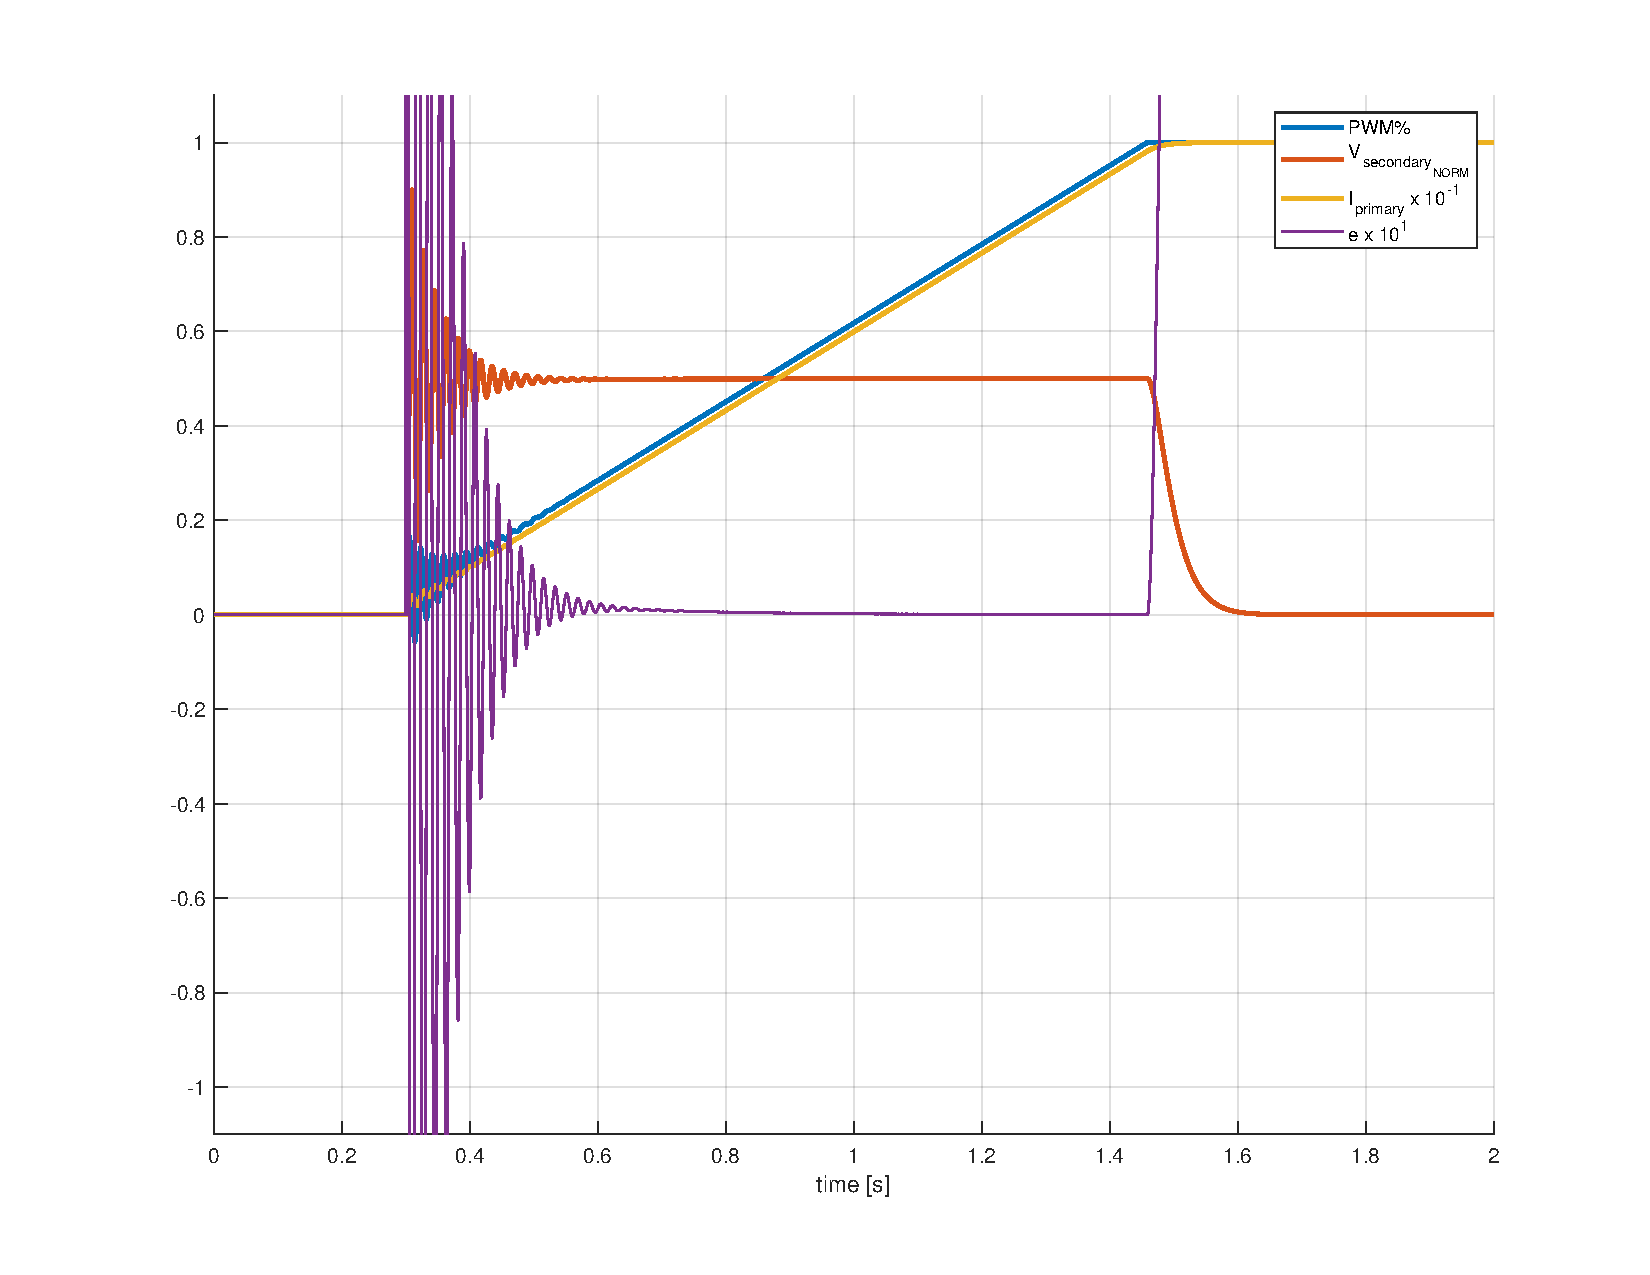
\includegraphics[width=1\textwidth]{ModelloMatematico/Simulation-cSim-Kp=0-K1=100-K2=500.pdf}
\end{figure}
\noindent
L'effetto è un ulteriore miglioramento sul \underline{Tempo di assestamento} e una una discesa più pronunciata dell'errore verso lo 0, ma abbiamo pagato questo incremento prestazionale con il ritorno degli effetti oscillatori smorzati, ed esse sono anche a frequenze maggiori, non proprio desiderabile. 

\newpage

\subsubsection{Analisi controllo Avanzato per $ K_p $=0.2 $ K_1 $=100 $ K_2 $=500}
Aggiungiamo quindi al caso precedente un termine proporzionale all'errore, così da rispondere subito alle variazioni del riferimento: 
\begin{figure}[H]
	\centering
	\caption[Controllo Avanzato $ K_p $=0.2 $ K_1 $=100 $ K_2 $=500]{Controllo Avanzato $ K_p $=0.2 $ K_1 $=100 $ K_2 $=500}
	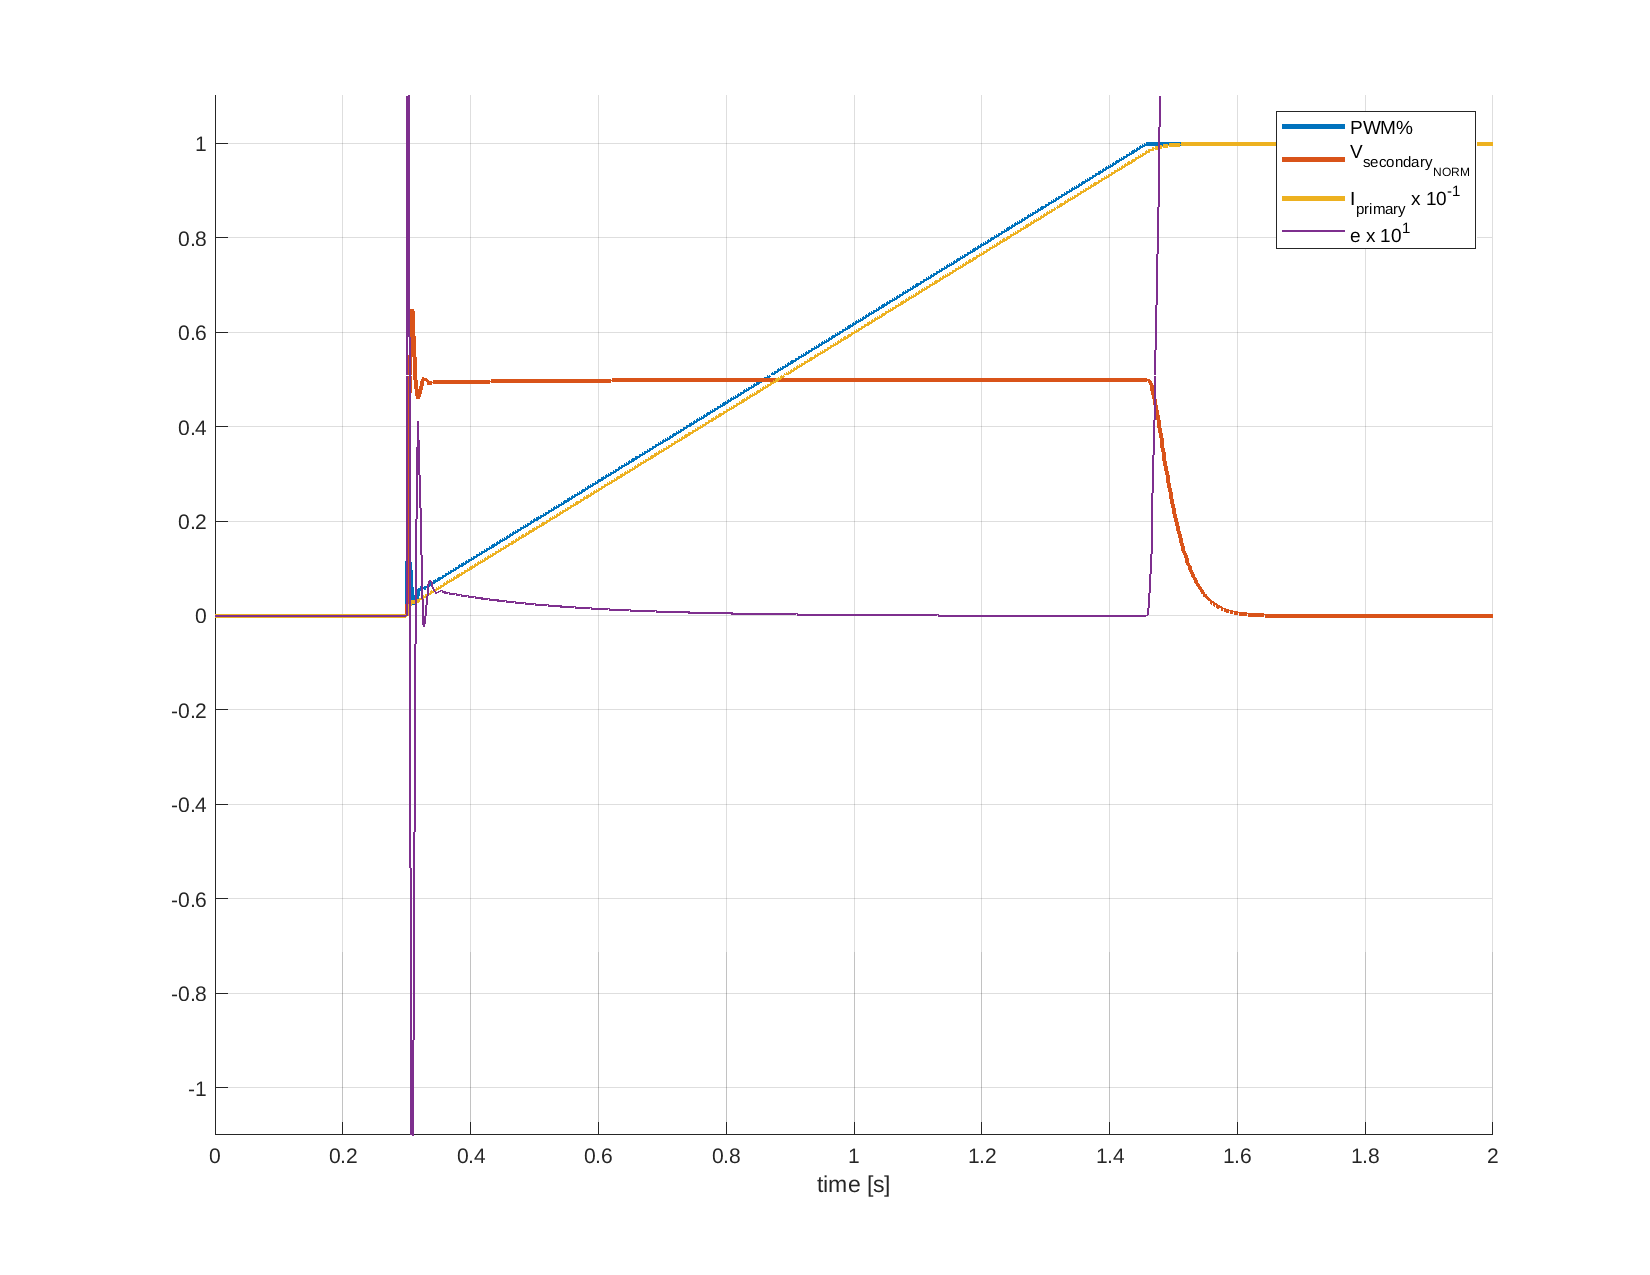
\includegraphics[width=1\textwidth]{ModelloMatematico/Simulation-cSim-Kp=0.2-K1=100-K2=500}
\end{figure}
\noindent
Essendo $ K_p $ istantaneo con la variazione del riferimento, abbiamo che l'inseguimento di $ V_{2_{ref}} $ inizia prima, riducendo il margine di fase dovuto al caricamento degli integratori, ciò riduce il fenomeno di wind-up presente precedentemente e causa delle oscillazioni attorno al riferimento, e permette di tornare al comportamento del 2° esperimento, con performance nettamente superiori.

\newpage

\subsubsection{Analisi controllo Avanzato per $ K_p $=0.8 $ K_1 $=100 $ K_2 $=500}
In quest'ultimo esperimento analizziamo l'effetto dell'aumento del termine proporzionale sulla dinamica:
\begin{figure}[H]
	\centering
	\caption[Controllo Avanzato $ K_p $=0.8 $ K_1 $=100 $ K_2 $=500]{Controllo Avanzato $ K_p $=0.8 $ K_1 $=100 $ K_2 $=500}
	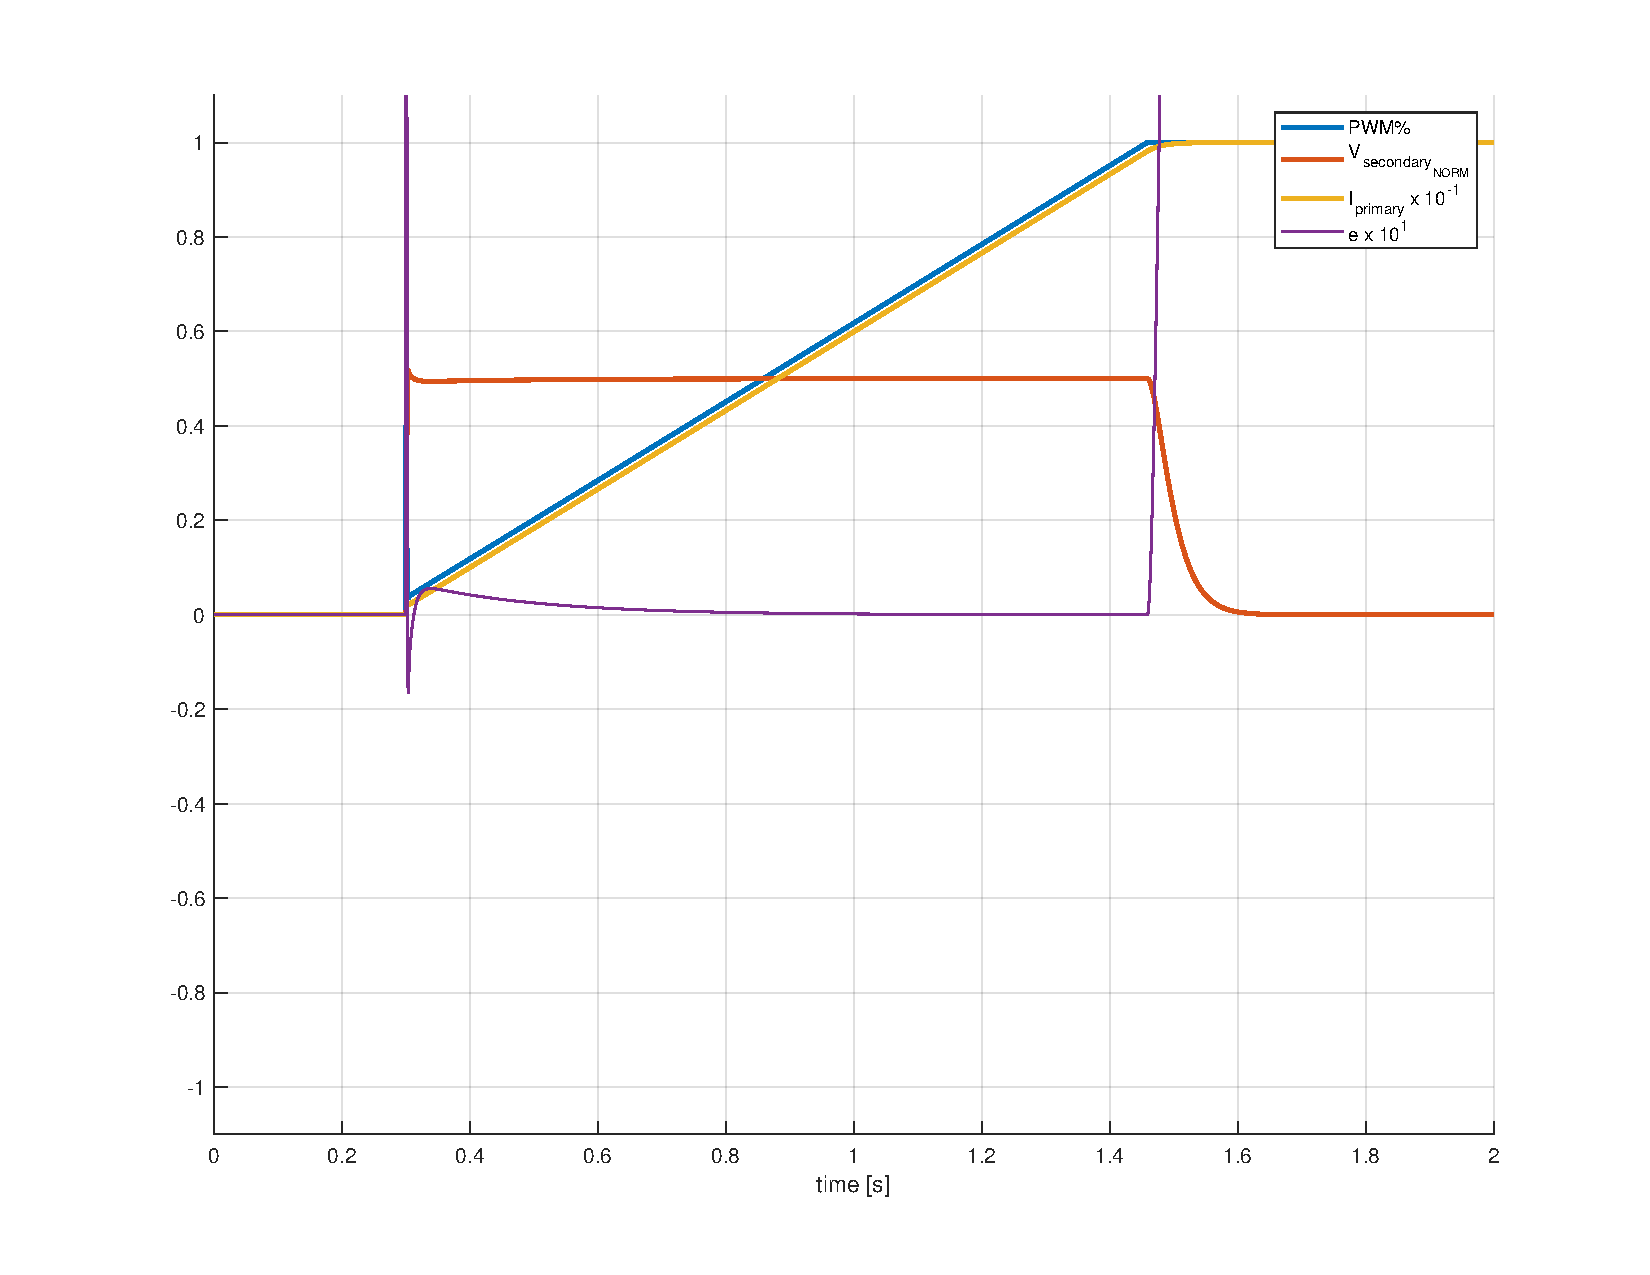
\includegraphics[width=1\textwidth]{ModelloMatematico/Simulation-cSim-Kp=0.8-K1=100-K2=500.pdf}
\end{figure}
\noindent
Rispetto al caso precedente, l'errore iniziale si è molto ridotto, passando da un fuori scala in entrambi i segni, a un errore di -0.019 di picco negativo (il picco positivo è per definizione 0.5 essendo il riferimento dato come gradino).\\
Al contrario, superata questa prima fase, il resto della dinamica è fondamentalmente identica al caso precedente.

\newpage

\section{Conclusioni per il design Avanzato} \label{sec:designControlloreConclusioni}
In conclusione possiamo dire che il controllore "\textit{PID-style}" definito nell'equazione \ref{eq:controllerDesign} permette di ottenere gli obiettivi di controllo prefissati, e i suoi coefficienti hanno un effetto sulle performance ottenibili.\\
La loro variazione ha il seguente effetto qualitativo:
\begin{description}
	\item[{\boldmath$ K_2 $}] Permette di raggiungere gli obiettivi di inseguimento con errore nullo, un suo aumento migliora la risposta ma causa delle oscillazioni smorzate a frequenze via via più elevate (Raggiungimento degli obiettivi di controllo).
	\item[{\boldmath$ K_1 $}] Se dimensionato opportunamente rende più marcato lo smorzamento delle oscillazioni dovute a $ K_2 $ fino a tornare ad un andamento esponenziale (Migliora Tempo di Assestamento).
	\item[{\boldmath$ K_p $}] Migliorare le performance nei primi istanti di controllo, prima che gli integratori possano arrivare a convergenza (Miglioramento del Tempo di risposta).
\end{description}

\begin{center}
	\rule{0.5\linewidth}{0.5px}
\end{center}
\noindent
I valori calcolati sul modello, non possono essere implementati 1:1 nel caso reale, a causa delle \nonLinearita che sono state trascurate nella creazione del modello, e per tutti i problemi dovuti al tempo di campionamento e attuazione del sistema che è pari a $ 2Khz $.\\
Non di meno, le osservazioni qui riportate continuano ad essere valide anche sul sistema reale, ed essendo le \nonLinearita presenti soprattutto nei pressi della \textit{Dead-zone} e della \textit{Saturazione} e assimilabili a del disturbo non troppo ampio, avremo modo di mostrare che il controllore così progettato è anche robusto per errori di attuazione e misura.




\chapter{Sviluppo Controllo reale}\label{cap:controlDevelop}

\begin{minipage}{12cm}\textit{
		In questo capitolo vedremo come è implementato nella realtà il controllore descritto nel capitolo \nameref{cap:controlModel} all'interno del \microControllore, tareremo i suoi coefficienti e mostreremo come si comporta in un esperimento reale con tutti i problemi ad esso connessi (\nonLinearita del \cite*{IBT-2}, errori di quantizzazione, discretizzazione del controllo, ecc...)
	}
\end{minipage}

%\vspace*{1cm}

\begin{figure}[H]
	\centering
	\caption[Impianto Reale]{Impianto Reale}
	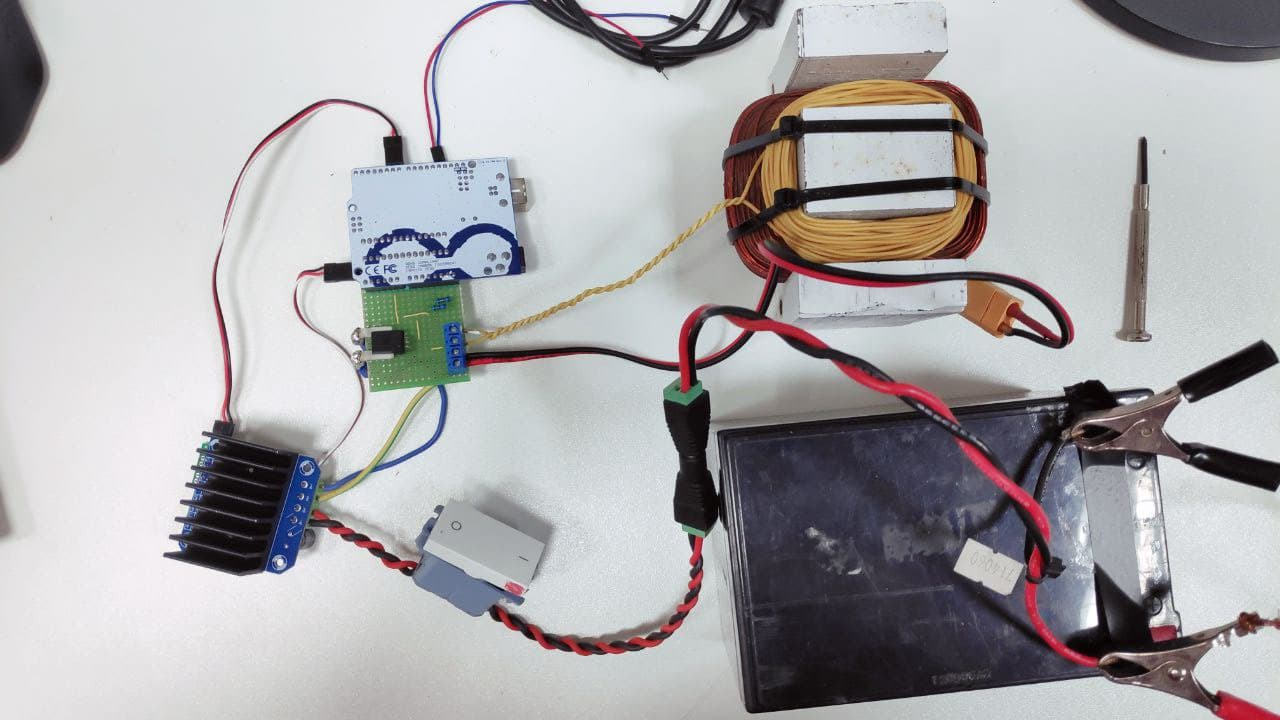
\includegraphics[width=1\textwidth]{ImpiantoReale.jpg}
\end{figure}
\noindent
Essendo un \microControllore un computer non eccessivamente potente, è necessario realizzare la funzione di trasferimento del il controllo (equazione \ref{eq:controllerDesign}) mediante un sistema a tempo discreto.\\
Per semplificarci l'implementazione, invece di creare un unico sistema del 2° ordine, si è optato per sommare tra loro le tre funzioni di trasferimento semplici che compongono il controllore, così da semplificare il debugging e permettere un più semplice controllo sullo stato dei componenti, utile per saturare gli integratori una volta che l'uscita ha superato la soglia di attuabilità (\textit{Saturazione}).\\
In fine, essendo l'obiettivo di controllo realizzato da una rampa, dopo un certo tempo in saturazione, per evitare lo spreco di energia da parte della batteria che alimenta il sistema, il codice disattiva il controllo, resetta tutti gli stati e mette il riferimento a 0. Questo stato non è permanente ma persiste fino al raggiungimento di un nuovo input di controllo mediante \cite*{EMP}.

\newpage
\section{Discretizzazione Zero-Order Hold (Z.O.H.)}
Un oggetto del tipo \textit{\textbf{Zero-Order Hold} (Z.O.H.)} altro non è che un convertitore Digitale$ \rightarrow $Analogico che permette di interfacciare dei segnali \textbf{Tempo Discreto} $\mathbb{T} =  \mathbb{Z} $ che evolvono $\forall \Delta T_s $\footnote{$ T_s $ = Sampling Time} con sistemi dinamici \textbf{Tempo Continuo} $\mathbb{T} =  \mathbb{R} $.

\begin{figure}[H]
	\centering
	\caption[Discretizzazione Zero-Order Hold  $ H_d(z) $ del sistema Tempo continuo $ H(s) $]{Discretizzazione ZOH $ H_d(z) $ per il sistema Tempo continuo $ H(s) $}
	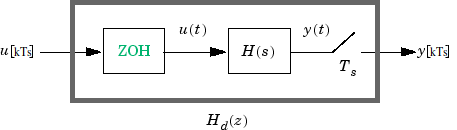
\includegraphics[width=1\textwidth]{Controllo/zoh-apply.png}
\end{figure}
\noindent
Questa interconnessione "\textit{congela}" l'ultimo segnale discreto $ u(k T_s) $ ricevuto e lo ripropone come un segnale costante in ingresso al sistema continuo che evolve in maniera indipendente.\\
L'uscita $ y(k T_s) $ è la discretizzazione di $ y(t) $, campionata ogni $ T_s $ .
\begin{figure}[H]
	\centering
	\caption[Effetto sui segnali discretizzati con il metodo Zero-Order Hold]{Segnali discretizzati con il metodo Zero-Order Hold}
	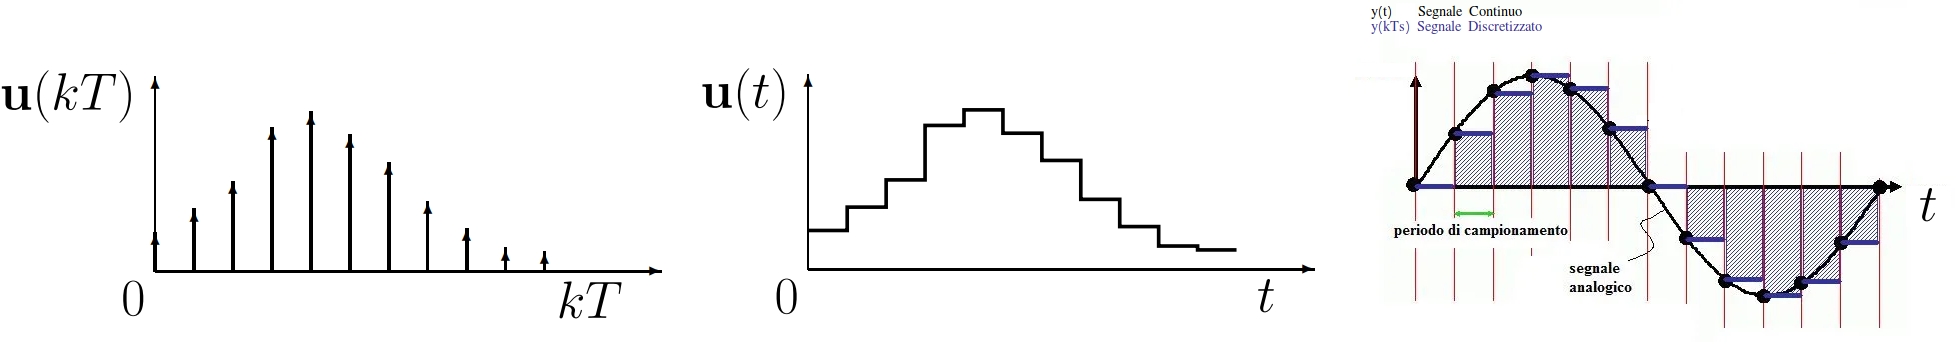
\includegraphics[width=1\textwidth]{Controllo/SegnaliDiscretiContinui.png}
\end{figure}
\noindent
Il sistema $ H(s) $ durante gli intervalli $ T_s $  evolve avendo una costante in ingresso, e al successivo istante di campionamento l'uscita raggiunta viene campionata e mantenuta per ul successivo $ T_s $, e questo procedimento all'infinito.
\newpage
\noindent
Ora che abbiamo descritto qualitativamente cosa avviene usando una discretizzazione ZOH, vediamo ora come diventa $ H_d(s) $ nello spazio di stato in termini matematici. Il procedimento di discretizzazione necessita di passare attraverso lo spazio di stato dei 3 sistemi dinamici che compongono il controllore \ref{eq:controllerDesign} e usando le formule del professore \cite{Discretizzazione}, si ottengono i risultati seguenti risultati:
\begin{table}[H]
	\centering
	\caption[Funzioni di trasferimento nello spazio di Stato, da Tempo Continuo a Tempo Discreto]{Funzioni di trasferimento nello spazio di Stato, da $ \mathbb{T} = \mathbb{R} \rightarrow \mathbb{T} = \mathbb{Z} $}\label{tab:discretizzazione}
	{\Large
		\begin{tabular}[t]{||c||c||c||}
			\hline
			                                                                          &                                        &                         \\[-3mm]
			$ C_{I^2}(s) = \frac{K_2}{s^2}$                                           & $ C_I(s) = \frac{K_1}{s}$              & $ C_p(s) = K_p $        \\[2mm]
			                                                                          &                                        &                         \\[-3mm]
			{\normalsize $ \left\{\begin{matrix}
					\dot{x} = & \begin{pmatrix}
						0 & 1 \\
						0 & 0
					\end{pmatrix} x & + & \begin{pmatrix}
						0 \\
						K_2
					\end{pmatrix} u \\
					          &                                                               \\[-1mm]
					y       = & \begin{pmatrix}
						1 & 0
					\end{pmatrix} x
				\end{matrix}\right. $
			}                                                                         &
			$ \left\{\begin{matrix}
					\dot{x} = & x & + K_1 \cdot u \\
					y       = & x &
				\end{matrix}\right.$

			                                                                          &
			$\left\{\begin{matrix}
					y = K_p \cdot u
				\end{matrix}\right. $                                                                                                   \\[9mm]
			\hline\hline
			                                                                          &                                        &                         \\[-3mm]
			{\normalsize $ \left\{\begin{matrix}
					x^+ = & {\small \begin{pmatrix}
								1 & T_s \\
								0 & 1
							\end{pmatrix}} \cdot x_k & + & K_2 {\small \begin{pmatrix}
						T_s^2/2 \\
						T_s
					\end{pmatrix}} u_k \\
					      &                                                                                                 \\[-1mm]
					y_k = & \begin{pmatrix}
						1 & 0
					\end{pmatrix} \cdot x_k
				\end{matrix}\right. $
			}                                                                         &
			{\normalsize $ \left\{\begin{matrix}
							x^+ = & x_k & + K_1 T_s \cdot u_k \\
							y_k = & x_k
						\end{matrix}\right.$

			}                                                                         &
			$\left\{\begin{matrix}
					y_k        = K_p \cdot u_k
				\end{matrix}\right. $                                                                                                  \\[9mm]
			                                                                          &                                        &                         \\[-3mm]
			$ C_{I^2}(z)|_{T_s} = K_2 \cdot \frac{T_s}{2} \cdot \frac{z+1}{(z -1)^2}$ & $ C_I(z)|_{T_s} = \frac{K_1 T_s}{z-1}$ & $ C_p(z)|_{T_s} = K_p $ \\[2mm]

			\hline
		\end{tabular}
	}%\Large
\end{table}\vspace{-3mm}
\noindent
Si può notare che in tutti e 3 i sistemi si è scelta una realizzazione della funzione di trasferimento nello Spazio di Stato tempo continuo in \textit{Forma Compagna di Osservabilità} (\cite{FormeCanoniche}).\\
Questa scelta non è stata casuale e ha lo scopo di semplificare in futuro la codifica per un sistema di controllo \textbf{Switching nei Coefficienti}, volto a migliorarne ulteriormente le prestazioni, senza dover scalare lo stato in base al cambio dei coefficienti.\\
Questa comoda proprietà è dovuta alla struttura della matrice $ C $, la quale, per variazioni \textbf{istantanee} dei coefficienti $ K_2,K_1,K_p$, non propaga gli effetti sull'uscita $ y(t) $, l'effetto della variazione arriverà in un secondo momento grazie all'integrazione dello stato, che ovviamente evolverà diversamente da prima a causa delle variazioni dei coefficienti. Per avere un idea qualitativa degli effetti dei coefficienti sul sistema complessivo, rifarsi alla sezione "\nameref{sec:designControlloreConclusioni}".\\
I calcoli della trasformata Zeta, sono presenti solo per completezza e sono stati ottenuti usando la classica formula:\vspace{-5mm}
\begin{center}
	{\Large 		$ G(z) = C_d \left(z I - A_d\right)^{-1} B_d + D_d $}
\end{center}
\noindent
Per i nostri scopi noi siamo interessati alle matrici $ A_d,B_d,C_d,D_d $ della conversione, così da implementare esattamente la discretizzazione di ordine Zero del sistema dinamico.\\
\vspace{-6mm}
\section{Codifica del controllore}\vspace{-4mm}
La codifica del controllore \ref{eq:controllerDesign} avviene attraverso le matrici $ A_d,B_d,C_d,D_d $ riportate in tabella \ref{tab:discretizzazione}, con queste matrici è stato costruito la classe di controllo \verb|iiCTRL| riportata in appendice nel codice del controllore (\nameref{lst:controlClassH} e \nameref{lst:controlClassCpp}).\\
La classe viene chiamata all'interno del \nameref{lst:controlLoop} ogni istante di campionamento, e permette la modifica a richiesta del riferimento da inseguire.\\
All'interno della classe è già codificata una la logica di \textit{Safe-Shutdown}, essa viene attivata quando il controllo ha raggiunto la saturazione per un tempo superiore ai 200ms, risulta infatti rischioso e dispendioso tenere connesso il trasformatore, poiché le correnti che scorrono sono dell'ordine dei 10A, e in ogni caso raggiungere gli obiettivi di controllo necessita di una rampa di corrente sul primario, che non si può ottenere se si è già saturato.\\
Questo contatore viene ripristinato a 0 all'arrivo di un nuovo riferimento da inseguire, causando di fatto il ripristino dell'esperimento.

%\newpage

\section{Esperimenti}
Di seguito vengono riportati diversi spari catturati dal sistema in funzione, nella sua interezza, usando al posto di \MARTe, un programma scritto in C++ per Linux chiamato \textit{MARTe2Moc}, quando il resto del sistema verrà controllato, gli stessi input di comando inviati da questa imitazione saranno ricevuti dal \microControllore e attuati in maniera identica.

\subsection{Inseguimento singolo}
In questo "\textit{sparo}" viene impostato il riferimento a $ V_{2_{ref}}=0.5V $ e il controllo insegue prontamente il riferimento, mantenendo l'errore entro margini molto stretti e con una decrescita esponenziale.\vspace{-2mm}
\begin{figure}[H]
	\centering
	\caption[Esperimento singolo $ V_{2_{ref}}=0.5V $]{Esperimento singolo $ V_{2_{ref}}=0.5V $}
	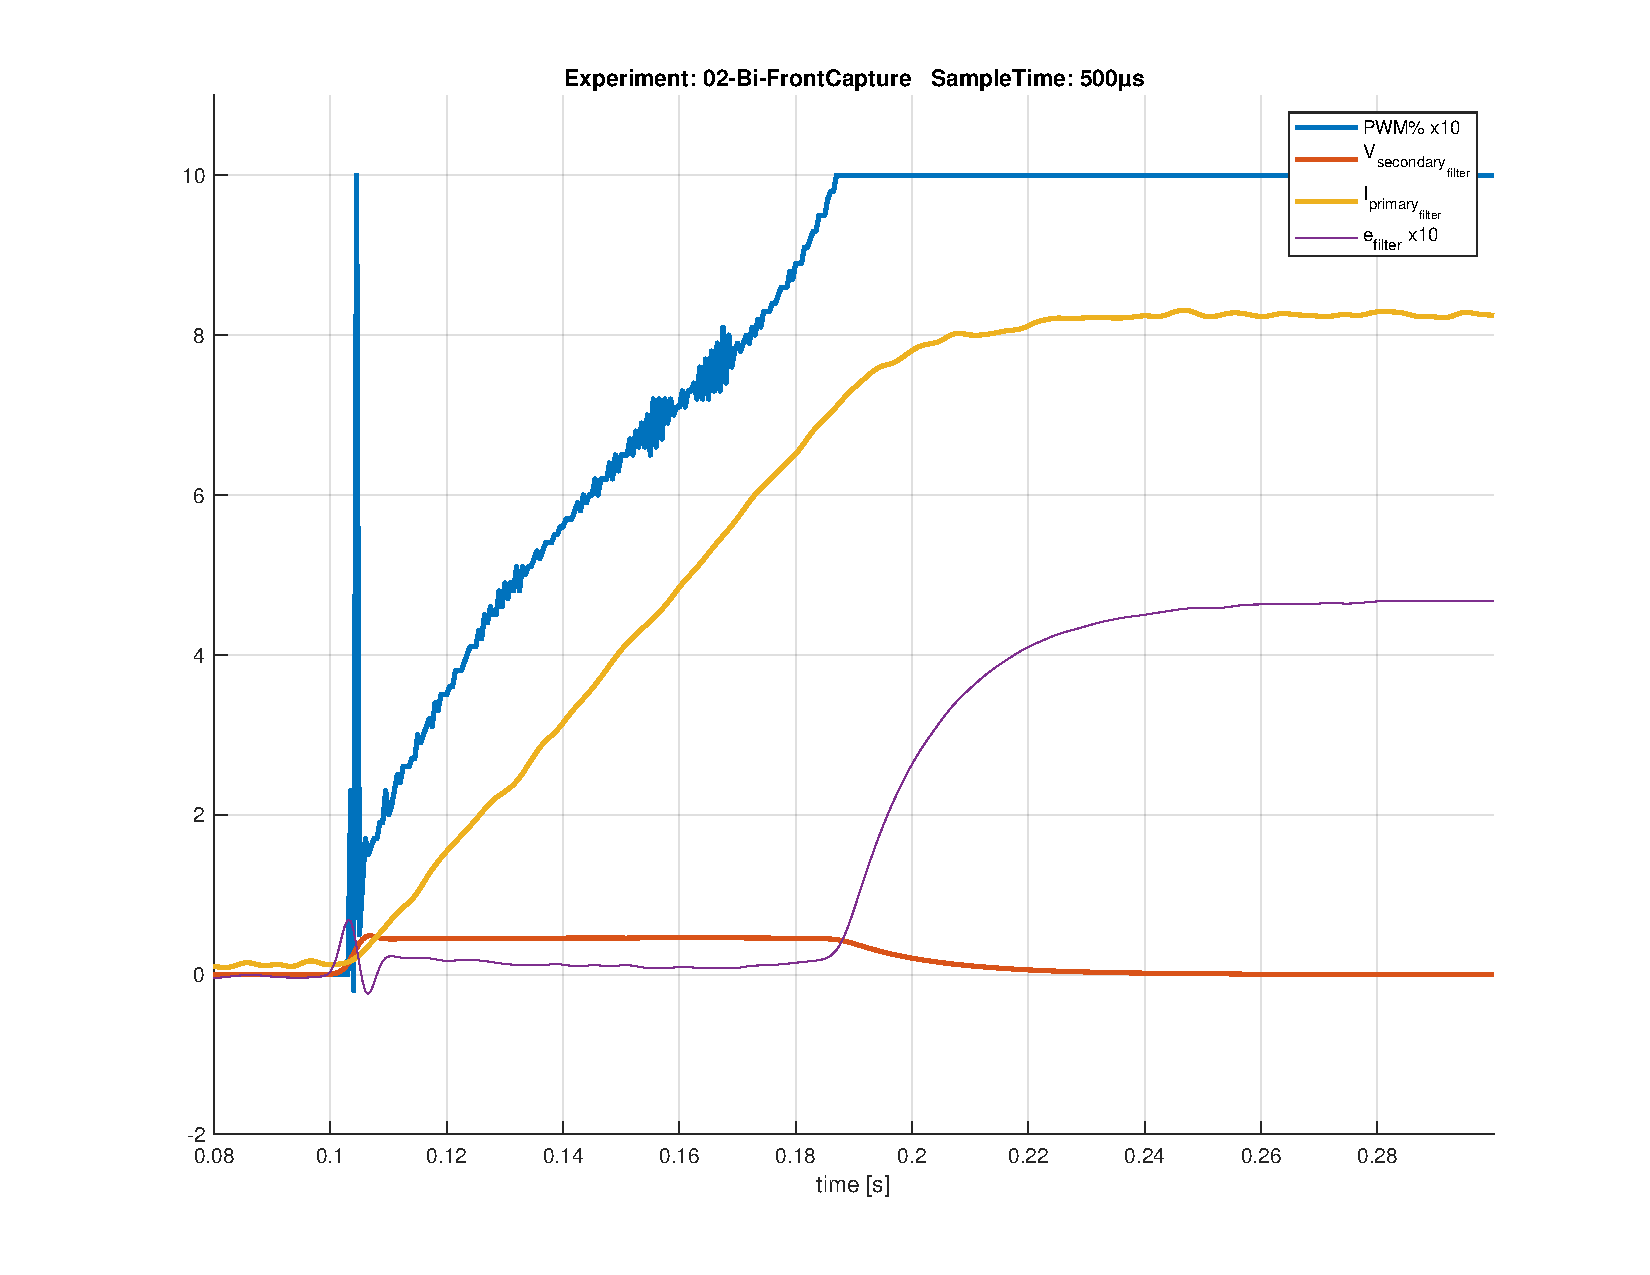
\includegraphics[width=1\textwidth]{Controllo/02-Bi-FrontCapture.pdf}
\end{figure}\vspace{-8mm}
\noindent
Come abbiamo avuto modo di vedere nel capitolo "\nameref{cap:stimaModello}", il modello lineare che abbiamo trovato, taglia tutta una serie di \nonLinearita presenti invece nell'impianto e particolarmente evidenti nei pressi della \textbf{Dead-Zone} e della \textbf{Saturazione}, ma il controllo in catena chiusa riesce a gestire questi problemi e il sistema sin dall'inizio tende a 0 esponenzialmente.\\
Passati i 200ms in saturazione il controllo automaticamente va a 0, realizzando la logica di \textit{Safe-Shutdown} descritta prima. Negli istanti subito successivi è possibile vedere come la tensione sul secondario vada fuori scala e si saturi attorno a $ -2.2V $, questo è concorde con i limiti di misura che abbiamo sul prototipo, e impone che le pendenze massime ineseguibili siano non superiori ai $ \pm2V $.

\subsection{Inseguimento Triangolare}
In questo secondo esperimento, \textit{MARTe2Moc} è stato programmato per invertire il segno del riferimento ogni volta che il controllo arriva in saturazione, l'obiettivo del test è vedere la risposta del controllo nei pressi della \textbf{Dead-Zone} e in corrispondenza di inversione di polarità, il continuo ribaltamento del $ V_{2_{ref}} $ impedisce di arrivare in saturazione troppo a lungo, rendendo l'esperimento periodico e illimitato nel tempo.\vspace{-2mm}
\begin{figure}[H]
	\centering
	\caption[Inseguimento Triangolare $ V_{2_{ref}}=\pm0.5V $]{Inseguimento Triangolare $ V_{2_{ref}}=\pm0.5V $}
	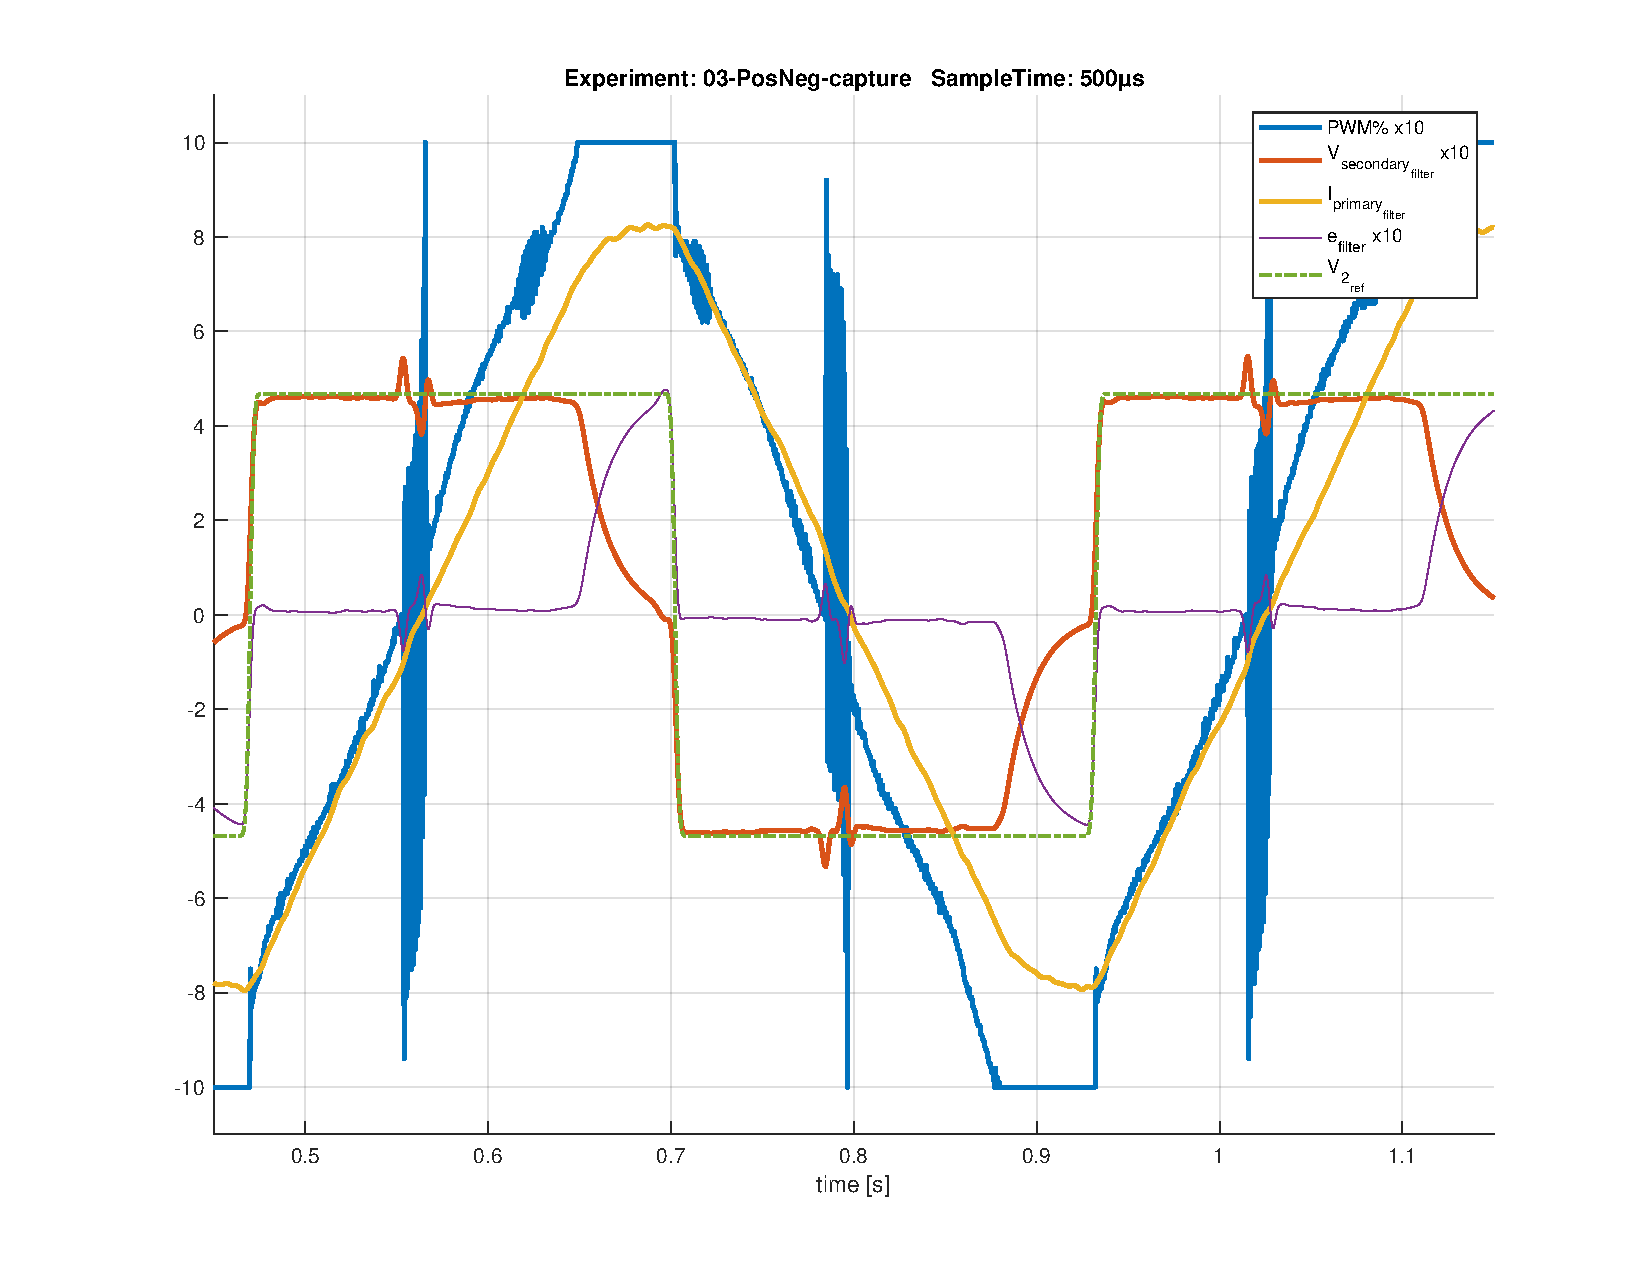
\includegraphics[width=1\textwidth]{Controllo/03-PosNeg-capture.pdf}
\end{figure}\vspace{-8mm}
\noindent
Come è possibile vedere, nei pressi della \textbf{Dead-Zone} la presenza della zona morta fa si che l'errore cresca di $ 0.02V $, ma questo errore viene rapidamente ripreso e portato in 0.\\

\newpage

\subsection{Cambio riferimento in corsa}
In questo terzo esperimento, \textit{MARTe2Moc} è stato programmato per inviare un nuovo riferimento casuale ogni 500ms, nel grafico riportato vi è stato prima un inseguimento "\textit{ripido}", seguito da uno molto morbido che è stato interrotto ben prima del raggiungimento della saturazione da un altro riferimento dello stesso segno negativo ma più ripido:\vspace{-2mm}
\begin{figure}[H]
	\centering
	\caption[Cambio di $ V_{2_{ref}} $ prima della saturazione]{Cambio di $ V_{2_{ref}} $ prima della saturazione}
	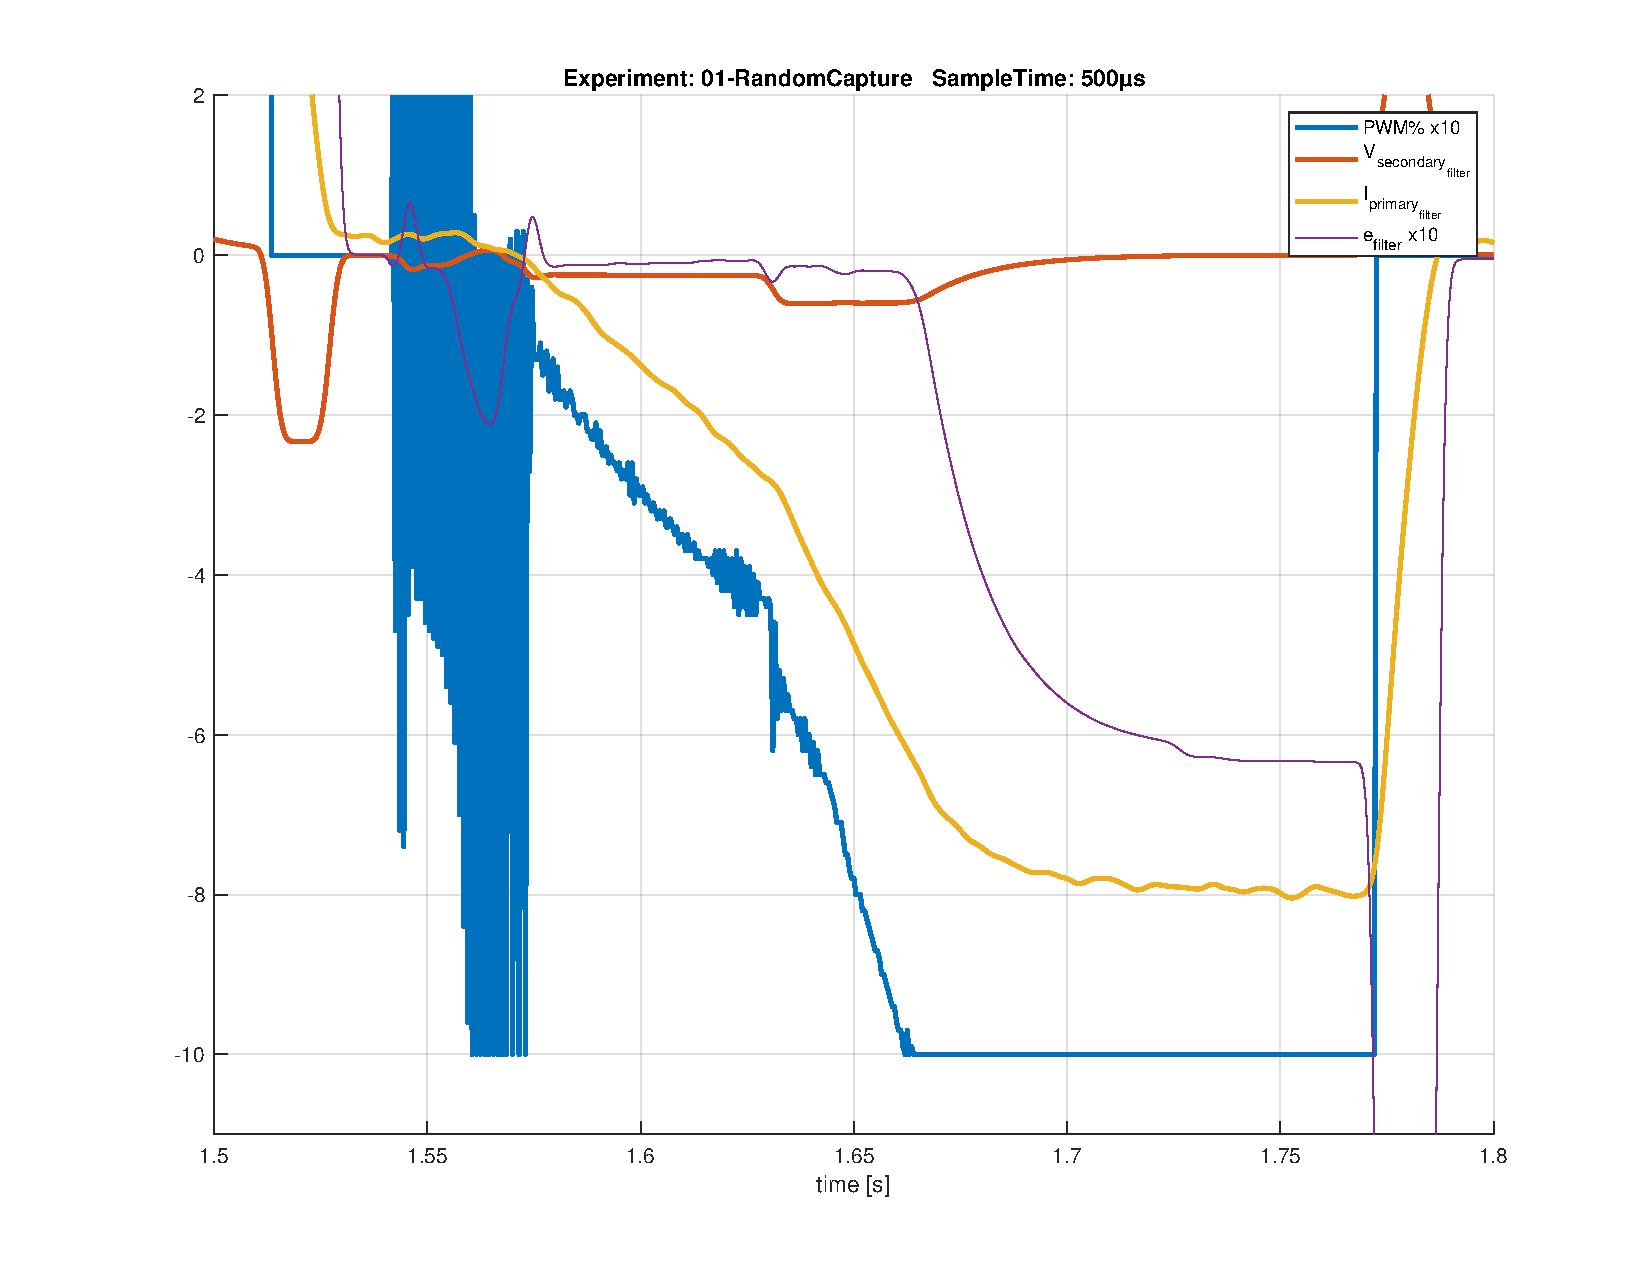
\includegraphics[width=1\textwidth]{Controllo/01-RandomCapture.pdf}
\end{figure}\vspace{-8mm}
\noindent
Risulta evidente che il sistema accetta bene i cambi di riferimenti, bisogna solo correggere il problema nella classe che implementa il controllore modificando che il cambio di riferimento non influisca sullo stato automaticamente.
\chapter{Conclusioni e sviluppi futuri}
\section*{Conclusioni}
In conclusione, con questo prototipo si è dimostrato e realizzato un controllore \textit{PID-style} a doppio Polo nell'origine, è un design di controllore perfetto da usare per governare la corrente di una bobina in un impianto Tokamak.\\
La realizzazione di questo prototipo però, come per ogni progetto pratico, ha dovuto confrontarsi con vari problemi di \nonLinearita, problemi implementativi, limiti di attuazione e campionamento, etc...\\
La risoluzione di questi problemi ha portato a compromessi e semplificazioni volte a catturare gli aspetti principali dell'esperimento, trascurando quelli secondari.\\
Il controllo così creato, oltre a funzionare bene nella teoria, risulta robusto alle variazioni dal modello lineare presenti nella realtà ma trascurate durante la modellizzazione del sistema, e ciò rende un simile design di controllo general-purple per impianti tokamak, poiché i coefficienti trovati nel corso di questa tesi permettono l'ottimizzazione per questo impianto in particolare, ma porterebbero a convergenza un qualunque impianto Tokamak avente la stessa struttura nella dinamica.\\

\section*{Sviluppi Futuri}
Anche se per i fini della tesi il progetto termina qui, il progetto in se ancora avanza, e tra gli sviluppi futuri abbiamo:
\begin{itemize}
	\item L'intenzione di portare un controllo \textbf{Switching} nella legge di Up-date, variando i coefficienti del controllore \ref{eq:controllerDesign}\\
	      In tal senso il controllore implementato nel \microControllore, ottenuto dal modello nello spazio di stato in Forma Compagna di Osservatore (\cite{FormeCanoniche}) già rende il sistema pronto per questo tipo di modifica a livello di codice, è necessario tuttavia studiare e simulare per quali soglie lo switch dei parametri può incrementare le performance, prima di poter implementare una simile tecnica.
	\item Attualmente è in cantiere la realizzazione all'interno di \MARTe della libreria \cite*{EMP} per permettere l'integrazione di questo firmware con l'ecosistema \MARTe.
	\item Risulta di interesse eseguire un upgrade del \microControllore dal'\ArduinoUno a una scheda più performante, e che permetta comunicazioni, campionamenti e PWM a velocità superiori, permetterebbe di superare l'attuale soglia di $ 2Khz $ di controllo, e realizzare dei controlli molto più performanti con tempi di campionamento molto inferiori, e quindi ritardi di fase ancora più azzerati.
	\item In fine, per raggiungere performance superiori è necessario avere un motore superiore, in questo caso il ponte-H, trovarne uno con una dinamica più lineare e che possa funzionare a frequenze maggiori di PWM permetterebbe di avere un controllo sul Primario molto più fine e potente, portando a migliorare le prestazioni in maniera sensibile e tangibile.

\end{itemize}






%% Programmi usati
%\chapter{Software, Toolchain, Strumenti}\label{cap:strumenti}
%Per la realizzazione di questa tesi sono stati usati:

\chapter*{Appendice A\\ Arduino Code}\label{ArduinoCode}
\addcontentsline{toc}{chapter}{Appendice A - Codice Arduino}

\section{Set-up Registri}

\subsubsection{Tic Timer}

\begin{lstlisting}[style=cppStyle,caption={Tic Timer},label=lst:ticTimer] 
	void periodicTask(int time) { 		// time in micro secondi
		// PWM pin Disable, motalita CTC(pt1)
		TCCR2A = (0x0 << COM2A0) | (0x0 << COM2B0) | (0x2 << WGM20);
		// CTC(pt2), Prescalere 256
		TCCR2B = (0 << WGM22) | (0x6 << CS20);                       
		// T_cklock * Twant / Prescaler = valore Registro
		OCR2A = (int)(16UL * time / 256);
		TIMSK2 = (1 << OCIE2A); // attivo solo l'interrupt di OC2A
	}
\end{lstlisting}
Questa funzione imposta il TIMER2 in modalità Fast PWM, ovvero che si resetta quando arriva al conteggio finale, e calcola il valore da mettere nel registro affinchè il conteggio sia il più vicino possibile a tempo desiderato

\subsubsection{Frequenza PWM}

\begin{lstlisting}[style=cppStyle,caption={Frequenza PWM},label=lst:pwmFreq] 
enum pwmFreq: char {
	hz30, hz120, hz490, hz4k, hz30k
};

void setMotFreq(pwmFreq freq) {
	// TCCR0B is for Timer 0
	#define myTimer TCCR0B
	switch (freq) {
		// set timer 3 divisor to  1024 for PWM frequency of    30.64 Hz
		case hz30:
			myTimer = (myTimer & B11111000) | B00000101;
		break;
		case hz120:
		// set timer 3 divisor to   256 for PWM frequency of   122.55 Hz
			myTimer = (myTimer & B11111000) | B00000100;
		break;
		case hz490:
		// set timer 3 divisor to    64 for PWM frequency of   490.20 Hz
			myTimer = (myTimer & B11111000) | B00000011;
		break;
		case hz4k:
		// set timer 3 divisor to     8 for PWM frequency of  3921.16 Hz
			myTimer = (myTimer & B11111000) | B00000010;
		break;
		case hz30k:
		// set timer 3 divisor to     1 for PWM frequency of 31372.55 Hz
			myTimer = (myTimer & B11111000) | B00000001;
		break;
		default:
			setMotFreq(hz4k);
		break;
	}
	#undef myTimer
}
\end{lstlisting}
Mediante questa funzione si modifica il valore del Prescaler per il TIMER 0, modificando la velocità di conteggio si ottiene un PWM con una periodo, e quindi frequenza, che varia.


\newpage

\section{Generatore di Segnale}

Per generare i segnali di controllo in Feed-Forward usati nel sistema, sono stati usati 2 diversi livelli di programmazione.\\
Un primo livello segnali di base, definiti su tutto $\mathbb{R}$, e usabili a piacere, e dei segnali compositi e periodici da mandare durante l'esperimento.
Tutti i segnali sono pensati per andare da -100\% <-> 100\%, è compito dell'attuazione
eliminare le deadzone e traslare il controllo al valore più opportuno

\subsection{Segnali Base}

\subsubsection{Rampa}
\begin{lstlisting}[style=cppStyle,caption={Rampa Saturata},label=lst:rampa] 
int ramp(uint64_t t, int vStart, uint64_t tStart, int vEnd, uint64_t tEnd) {
	// Saturazione
	if (t < tStart)
		return vStart;
	else if (t > tEnd)
		return vEnd;
	// Retta
	unsigned int dt = t - tStart;
	return vStart + int((vEnd - vStart) / float(tEnd - tStart) * dt);
}
\end{lstlisting}
La rampa è descritta come una retta nell'intervallo di interesse, saturata prima e dopo il tempo desiderato\\
$ RampaSat(t) =
	\left \{ \begin{array}{l c}
		v_{start} + \frac{v_{end}-v_{start}}{t_{end}-t_{start}} * (t - t_{start}) & \forall t \in [t_{start},t_{end}] \\
		v_{start}                                                                 & t<t_{start}                       \\
		v_{end}                                                                   & t>t_{start}
	\end{array}
	\right.
$

\newpage
\subsection{Segnali Composti}

\subsubsection{Onda Triangloare}
\begin{lstlisting}[style=cppStyle,caption={Onda Triangolare Periodica},label=lst:ondaTriangloare] 
int triangleSignal(uint64_t t, int msQuartPeriod) {
	static uint64_t startTic = 0;
	int dTic = t - startTic;
	int pwm = 0;
	if (dTic < ticConvert(msQuartPeriod))
		pwm = ramp(dTic, 0, 0, 100, ticConvert(msQuartPeriod));
	else if (dTic < (ticConvert(msQuartPeriod) * 3))
		pwm = ramp(dTic, 100, ticConvert(msQuartPeriod), -100, ticConvert(msQuartPeriod) * 3);
	else if (dTic < (ticConvert(msQuartPeriod) * 4))
		pwm = ramp(dTic, -100, ticConvert(msQuartPeriod) * 3, 0, ticConvert(msQuartPeriod) * 4);
	else {
		pwm = 0;
		startTic = t;
	}
	return pwm;
}
\end{lstlisting}

\subsubsection{Onda Trapezoidale}
\begin{lstlisting}[style=cppStyle,caption={Onda Trapezoidale Periodica},label=lst:ondaTrapezoidale] 
int rapidShot(uint64_t t) {
	static uint64_t startTic = 0;
	int pwmRapidShot;
	long dTic = t - startTic;
	if (dTic > t4) {
		startTic = t;
		pwmRapidShot = 0;
		dTic = t - startTic;
	}
	
	if (dTic <= t1) {
		pwmRapidShot = ramp(dTic, 0, 0, 100, t1);
	} else if (dTic <= t2) {
		pwmRapidShot = 100;
	} else if (dTic <= t3) {
		// falling ramp
		pwmRapidShot = ramp(dTic, 100, t2, 0, t3);
	} else if (dTic <= t4) {
		pwmRapidShot = 0;
	}	
	return pwmRapidShot;
}
\end{lstlisting}


\chapter*{Appendice B\\ EMP Code}\label{EMPCode}
\addcontentsline{toc}{chapter}{Appendice B - Codice EMP}

\chapter*{Appendice C\\ Matlab Post Elaborazione}\label{MatlabCode}
\addcontentsline{toc}{chapter}{Appendice C - Matlab Post Elaboration}

% ELENCO DELLE FIGURE (OPZIONALE)
% Lista figure SENZA link colorati
{
	\hypersetup{hidelinks}% Rimuove la colorazione per i Link
	\listoffigures
	\addcontentsline{toc}{chapter}{Elenco delle figure}
}


% ELENCO DELLE TABELLE (OPZIONALE)
% Lista tabelle SENZA link colorati
{
	\hypersetup{hidelinks}% Rimuove la colorazione per i Link
	\listoftables
	\addcontentsline{toc}{chapter}{Elenco delle tabelle}
}


% ELENCO DEI CODICI (OPZIONALE)

% Lista Codici SENZA link colorati
{
	\hypersetup{hidelinks}% Rimuove la colorazione per i Link
	\lstlistoflistings
	\addcontentsline{toc}{chapter}{Elenco dei codici}
}

% BIBLIOGRAFIA
\printbibliography
\addcontentsline{toc}{chapter}{Bibliografia}





%\addcontentsline{toc}{chapter}{Bibliografia}
%\begin{thebibliography}{99}
%	\bibitem{bib1}Nome Autore,
%	\emph{``Nome del libro''},
%	Nome Editore, Anno di Pubblicazione.
%	\bibitem{bib2}C. Bonivento - C. Melchiorri - R. Zanasi,
%	\emph{``Sistemi di controllo digitale''},
%	Progetto Leonardo, 1995.
%	\bibitem{IBT2} Driver-Current datasheet\\ \footnotesize\url{https://www.datsi.fi.upm.es/docencia/Informatica_Industrial/DMC/IBT2.pdf}
%\end{thebibliography}

\end{document}
